%
%  thesis.tex  2011-07-01  Mark Senn  http://engineering.purdue.edu/~mark
%
%  This is the thesis ``root file''.
%
%  To print the final copy of your thesis put a '%'
%  in front of the \includeonly command and type
%  (from page 71 of _LaTeX User's Guide and Reference Manual_, 2nd edition):
%      latex thesis
%      bibtex thesis
%      latex thesis
%      latex thesis
%
%  In "Reference:" listings below:
%      KEY  MEANING
%      TM   ``A Manual for the Preparation of Graduate Theses'',
%             seventh revised edition, The Graduate School, 2006.
%             http://www2.itap.purdue.edu/gradschool//Publications/graduate-thesis-manual.pdf
%      PU   ``A Manual for the Preparation of Graduate Theses'',
%           The Graduate School, Purdue University, 1996.
%           http://www2.itap.purdue.edu/gradschool//Publications/graduate-thesis-manual.pdf
%
%  Search for "CHANGE" below and change things as necessary.
%  I recommend putting "%%" before any existing lines that
%  need to be changed and adding your new line(s) immediately
%  below the existing lines.
%

% See http://www.ecn.purdue.edu/~mark/puthesis/#Options
% for documentclass options.
% CHANGE NEXT LINE?
\documentclass[ece,thesis]{puthesis}

% Define "align" environment used in demo-mathematics.tex.
% CHANGE NEXT LINE?
\usepackage{amsmath}

% Define "multicols" environment environment used in demo-multicols.tex.
% CHANGE NEXT LINE?
\usepackage{multicol}

% Define "subfigure" environment used in "demo-figure.tex".
% CHANGE NEXT LINE?
% \usepackage{subfigure}

% put boxes around our figures
\usepackage{float}
%\floatstyle{boxed}
%\restylefloat{figure}

% to get figures with side captions, and wrap text around figures
% https://en.wikibooks.org/wiki/LaTeX/Floats,_Figures_and_Captions
\usepackage{sidecap}
\usepackage{wrapfig}

% include subfigures for pageobjects.tex
% added style=base to help deal with compiler warning
% for unsupported document class
% using setspace so we can set our captions to be single spaced,
% not sure why they became unsingle spaced.
\usepackage[style=base]{caption}
\usepackage{subcaption}
\usepackage{setspace}


% Define "graphicx" environment used in "casestudy3.tex".
\usepackage{graphicx}

% Define "fontenc" environment used to angle brackets
% see http://texblog.net/latex-archive/fonts/symbols/
\usepackage[T1]{fontenc}

% packages for \code command in mydefs
% for code blocks to use Courier New
% \usepackage{fontspec}
% for code block colors
\usepackage[usenames,dvipsnames,svgnames,table]{xcolor}
% for code block writing text in a drawing
\usepackage{tikz}
% for code block syntax highlighting?
\usepackage{listings}

% Define "enumerate" environment for numbered lists
\usepackage{enumerate}

% Define environment for building outlines
% temporarily needed for hubzero.tex
\usepackage{outlines}
\usepackage{enumitem}

% for code listings, defined in mydefs.tex
\usepackage{courier}

% for problems.tex minipage environment
%\usepackage[floatraw]{chemstyle}
%\usepackage{chemstyle}

% include tables that wrap text in columns
\usepackage{tabularx}

% include clever references, automatic names before
% section/chapter/appendix references
\usepackage{cleveref}


% include url package for online citations
\usepackage{url}

% By default the URLs are put in typewriter type in the body and the
% bibliography of the document when using the \url command.  If you are
% using many long URLs you may want to uncommennt the next line so they
% are typeset a little smaller.
% \renewcommand{\UrlFont}{\small\tt}



% Title of thesis (used on cover and in abstract).
% The title shown must be the full, official title of the
% thesis.  Superscripts and subscripts are not permitted in
% the title.
% Reference: TM 26.
% Use \title{Put Title Here} for a one-line title.
% Use \\ to separate lines.
% Put % at the end of the last line to avoid getting an extra space
% in the abstract.
% There are two forms of title: one line or more than one line.
% There are examples of both below.
% Only use one \title.
% CHANGE NEXT FOUR LINES.
%%\title{An Example Thesis Done with LaTeX}
%%\title{%
%%  An Example Thesis Done with LaTeX\\
%%  with a Very Long Title%
%%}
\title{HUBcheck: Check the Hub}

% First author name with first name first is used for cover.
% Second author name with last name first is used for abstract.
% Your full name as it appears in the University records appears
% on the cover.
% Reference: TM 26, 29.
% There are two forms of author, with and without initials.
% There are examples of both below.
% Only use one \author line.
% CHANGE NEXT TWO LINES.
%%\author{Mark Senn}{Senn, Mark}
%%\author{Mark D. Senn}{Senn, Mark D.}
\author{Derrick S. Kearney}{Kearney, Derrick S.}

% First is long title of degree (used on cover).
% Second is abbreviation for degree (used in abstract).
% Third is the month the degree was (will be) awarded (used on cover
% and abstract).
% Last is the year the degree was (wlll be) awarded (used on cover
% and abstract).
% The degree title for all doctoral candidates is ``Doctor of Philosophy.''
% The precise degree names for master's candidates appear in the list of
% ``Degrees Offered'' in the Graduate School bulletin.
% The date is the month and year that the degree is actually awarded.
% (If you have registered for ``degree only,'' revise the thesis title
% page to reflect the new date on which the degree is to be awarded.)
% Reference: TM 26--27, 30.
% CHANGE NEXT LINE?
%%\pudegree{Doctor of Philosophy}{Ph.D.}{May}{2007}
\pudegree{Master of Science in Electrical and Computer Engineering}{M.S.E.C.E.}{May}{2015}

% Major professor (used in abstract).
% Use, for example:
%     \majorprof{John Q. Professor}
%     \majorprofs{John Q. Professor and Thomas R. Jones}
%     \majorprofs{John Q. Professor, Thomas R. Jones, and David S. Smith}
% depending on the number of major professors you have.
% CHANGE NEXT LINE.
%%\majorprof{John Q. Professor}
\majorprof{Sam Midkiff}

% Campus (used only on cover)
% Use one of the following:
%     Fort Wayne
%     Hammond
%     Indianapolis
%     West Lafayette
%     Westville
% Reference: TM 27.
% CHANGE NEXT LINE?
\campus{West Lafayette}

% My command definitions not specific to my thesis.
% CHANGE NEXT LINE?
%
%  mydefs.tex  2007-03-19  Mark Senn  http://www.ecn.purdue.edu/~mark
%
%  Command definitions that can be used in all documents that have
%      %
%  mydefs.tex  2007-03-19  Mark Senn  http://www.ecn.purdue.edu/~mark
%
%  Command definitions that can be used in all documents that have
%      %
%  mydefs.tex  2007-03-19  Mark Senn  http://www.ecn.purdue.edu/~mark
%
%  Command definitions that can be used in all documents that have
%      \input{mydefs}
%

%%%%%%%%%%%%%%%%%%%%%%%%%%%%%%%%%%%%%%%%%%%%%%%%%%
% setup code single spacing caption for all floats

\captionsetup{
  font={stretch=1},
}

%%%%%%%%%%%%%%%%%%%%%%%%%%%%%%%%%%%%%%%%%%%%%%%%%%


%%%%%%%%%%%%%%%%%%%%%%%%%%%%%%%%%%%%%%%%%%%%%%%%%%
% setup special fonts/format (xformat,xf) for talking about:
%   module
%   classes
%   class methods
%   class attributes (data members)
%   objects
%   locator
%   locator family
%   inline code
%   html link name
%   parameter name
%   uri scheme (http, https, mailto, webdav)
%   program name

\newcommand{\xfmodule}[1]{\texttt{#1}}
\newcommand{\xfclass}[1]{\texttt{#1}}
\newcommand{\xfmethod}[1]{\texttt{#1}}
\newcommand{\xfattribute}[1]{\texttt{#1}}
\newcommand{\xfobject}[1]{\texttt{#1}}
\newcommand{\xflocator}[1]{\texttt{#1}}
\newcommand{\xflocfam}[1]{\texttt{#1}}
\newcommand{\xfinlinecode}[1]{\texttt{#1}}
\newcommand{\xfhtmllink}[1]{\texttt{#1}}
\newcommand{\xfparameter}[1]{\texttt{#1}}
\newcommand{\xfurischeme}[1]{\texttt{#1}}
\newcommand{\xfprogramname}[1]{\textbf{#1}}


%%%%%%%%%%%%%%%%%%%%%%%%%%%%%%%%%%%%%%%%%%%%%%%%%%


%%%%%%%%%%%%%%%%%%%%%%%%%%%%%%%%%%%%%%%%%%%%%%%%%%
% setup code listing captions
%
% i could never figure out why the colorbox seems so indented
% so we just multiply our fboxsep by 7 and that accounts for
% the indentation. had to adjust framexleftmargin and
% framexrightmargin to match.
%

\DeclareCaptionFont{white}{\color{white}}
\DeclareCaptionFormat{listing}{
  \colorbox[cmyk]{0.43, 0.35, 0.35, 0.01}{
    \parbox{\dimexpr\textwidth-7\fboxsep\relax} {
      #1#2#3
    }
  }
}

\captionsetup[lstlisting]{
  format=listing,
  labelfont=white,
  textfont=white,
  singlelinecheck=false,
  margin=0pt,
}

%%%%%%%%%%%%%%%%%%%%%%%%%%%%%%%%%%%%%%%%%%%%%%%%%%


%%%%%%%%%%%%%%%%%%%%%%%%%%%%%%%%%%%%%%%%%%%%%%%%%%
% setting for code listings

\lstset{ %
  basicstyle=\scriptsize\ttfamily,    % the size of the fonts that are used for the code
  breaklines=true,                    % sets automatic line breaking
  captionpos=t,                       % sets the caption-position to bottom
  belowcaptionskip=15px,              % add some space under the caption and above the code
  frame=lines,                        % adds a frame around the code
  numbers=left,                       % where to put the line-numbers; possible values are (none, left, right)
  numbersep=5pt,                      % how far the line-numbers are from the code
  numberstyle=\tiny\color{black},     % the style that is used for the line-numbers
  showspaces=false,                   % show spaces everywhere adding particular underscores;
  showstringspaces=false,             % underline spaces within strings only
  showtabs=false,                     % show tabs within strings adding particular underscores
  stepnumber=1,                       % the step between two line-numbers. If it's 1, each line will be numbered
  stringstyle=\color{black}\ttfamily\textbf, % string literal style
  tabsize=2,                          % sets default tabsize to 2 spaces
  xleftmargin=5ex,                    % space between page margin and line numbers/code/frames
  framexleftmargin=13pt,               % left width of tob/bottom frame, starts at code, excludes line numbers
  framexrightmargin=-3pt,              % right width of top/bottom frame, starts at textwidth?
%  framexbottommargin=5pt,
  extendedchars=true,
  belowskip=15pt,
}

% load languages we will be using
\lstloadlanguages{
  XML,
  HTML,
  Python,
}

\lstnewenvironment{xcode}[1]
  {
    \noindent
    \minipage{\linewidth}
%    \lstset{tabsize=4, belowcaptionskip=1\baselineskip, #1}
    \lstset{tabsize=4, #1}
  }%
  {
    \endminipage
  }

%%%%%%%%%%%%%%%%%%%%%%%%%%%%%%%%%%%%%%%%%%%%%%%%%%

%

%%%%%%%%%%%%%%%%%%%%%%%%%%%%%%%%%%%%%%%%%%%%%%%%%%
% setup code single spacing caption for all floats

\captionsetup{
  font={stretch=1},
}

%%%%%%%%%%%%%%%%%%%%%%%%%%%%%%%%%%%%%%%%%%%%%%%%%%


%%%%%%%%%%%%%%%%%%%%%%%%%%%%%%%%%%%%%%%%%%%%%%%%%%
% setup special fonts/format (xformat,xf) for talking about:
%   module
%   classes
%   class methods
%   class attributes (data members)
%   objects
%   locator
%   locator family
%   inline code
%   html link name
%   parameter name
%   uri scheme (http, https, mailto, webdav)
%   program name

\newcommand{\xfmodule}[1]{\texttt{#1}}
\newcommand{\xfclass}[1]{\texttt{#1}}
\newcommand{\xfmethod}[1]{\texttt{#1}}
\newcommand{\xfattribute}[1]{\texttt{#1}}
\newcommand{\xfobject}[1]{\texttt{#1}}
\newcommand{\xflocator}[1]{\texttt{#1}}
\newcommand{\xflocfam}[1]{\texttt{#1}}
\newcommand{\xfinlinecode}[1]{\texttt{#1}}
\newcommand{\xfhtmllink}[1]{\texttt{#1}}
\newcommand{\xfparameter}[1]{\texttt{#1}}
\newcommand{\xfurischeme}[1]{\texttt{#1}}
\newcommand{\xfprogramname}[1]{\textbf{#1}}


%%%%%%%%%%%%%%%%%%%%%%%%%%%%%%%%%%%%%%%%%%%%%%%%%%


%%%%%%%%%%%%%%%%%%%%%%%%%%%%%%%%%%%%%%%%%%%%%%%%%%
% setup code listing captions
%
% i could never figure out why the colorbox seems so indented
% so we just multiply our fboxsep by 7 and that accounts for
% the indentation. had to adjust framexleftmargin and
% framexrightmargin to match.
%

\DeclareCaptionFont{white}{\color{white}}
\DeclareCaptionFormat{listing}{
  \colorbox[cmyk]{0.43, 0.35, 0.35, 0.01}{
    \parbox{\dimexpr\textwidth-7\fboxsep\relax} {
      #1#2#3
    }
  }
}

\captionsetup[lstlisting]{
  format=listing,
  labelfont=white,
  textfont=white,
  singlelinecheck=false,
  margin=0pt,
}

%%%%%%%%%%%%%%%%%%%%%%%%%%%%%%%%%%%%%%%%%%%%%%%%%%


%%%%%%%%%%%%%%%%%%%%%%%%%%%%%%%%%%%%%%%%%%%%%%%%%%
% setting for code listings

\lstset{ %
  basicstyle=\scriptsize\ttfamily,    % the size of the fonts that are used for the code
  breaklines=true,                    % sets automatic line breaking
  captionpos=t,                       % sets the caption-position to bottom
  belowcaptionskip=15px,              % add some space under the caption and above the code
  frame=lines,                        % adds a frame around the code
  numbers=left,                       % where to put the line-numbers; possible values are (none, left, right)
  numbersep=5pt,                      % how far the line-numbers are from the code
  numberstyle=\tiny\color{black},     % the style that is used for the line-numbers
  showspaces=false,                   % show spaces everywhere adding particular underscores;
  showstringspaces=false,             % underline spaces within strings only
  showtabs=false,                     % show tabs within strings adding particular underscores
  stepnumber=1,                       % the step between two line-numbers. If it's 1, each line will be numbered
  stringstyle=\color{black}\ttfamily\textbf, % string literal style
  tabsize=2,                          % sets default tabsize to 2 spaces
  xleftmargin=5ex,                    % space between page margin and line numbers/code/frames
  framexleftmargin=13pt,               % left width of tob/bottom frame, starts at code, excludes line numbers
  framexrightmargin=-3pt,              % right width of top/bottom frame, starts at textwidth?
%  framexbottommargin=5pt,
  extendedchars=true,
  belowskip=15pt,
}

% load languages we will be using
\lstloadlanguages{
  XML,
  HTML,
  Python,
}

\lstnewenvironment{xcode}[1]
  {
    \noindent
    \minipage{\linewidth}
%    \lstset{tabsize=4, belowcaptionskip=1\baselineskip, #1}
    \lstset{tabsize=4, #1}
  }%
  {
    \endminipage
  }

%%%%%%%%%%%%%%%%%%%%%%%%%%%%%%%%%%%%%%%%%%%%%%%%%%

%

%%%%%%%%%%%%%%%%%%%%%%%%%%%%%%%%%%%%%%%%%%%%%%%%%%
% setup code single spacing caption for all floats

\captionsetup{
  font={stretch=1},
}

%%%%%%%%%%%%%%%%%%%%%%%%%%%%%%%%%%%%%%%%%%%%%%%%%%


%%%%%%%%%%%%%%%%%%%%%%%%%%%%%%%%%%%%%%%%%%%%%%%%%%
% setup special fonts/format (xformat,xf) for talking about:
%   module
%   classes
%   class methods
%   class attributes (data members)
%   objects
%   locator
%   locator family
%   inline code
%   html link name
%   parameter name
%   uri scheme (http, https, mailto, webdav)
%   program name

\newcommand{\xfmodule}[1]{\texttt{#1}}
\newcommand{\xfclass}[1]{\texttt{#1}}
\newcommand{\xfmethod}[1]{\texttt{#1}}
\newcommand{\xfattribute}[1]{\texttt{#1}}
\newcommand{\xfobject}[1]{\texttt{#1}}
\newcommand{\xflocator}[1]{\texttt{#1}}
\newcommand{\xflocfam}[1]{\texttt{#1}}
\newcommand{\xfinlinecode}[1]{\texttt{#1}}
\newcommand{\xfhtmllink}[1]{\texttt{#1}}
\newcommand{\xfparameter}[1]{\texttt{#1}}
\newcommand{\xfurischeme}[1]{\texttt{#1}}
\newcommand{\xfprogramname}[1]{\textbf{#1}}


%%%%%%%%%%%%%%%%%%%%%%%%%%%%%%%%%%%%%%%%%%%%%%%%%%


%%%%%%%%%%%%%%%%%%%%%%%%%%%%%%%%%%%%%%%%%%%%%%%%%%
% setup code listing captions
%
% i could never figure out why the colorbox seems so indented
% so we just multiply our fboxsep by 7 and that accounts for
% the indentation. had to adjust framexleftmargin and
% framexrightmargin to match.
%

\DeclareCaptionFont{white}{\color{white}}
\DeclareCaptionFormat{listing}{
  \colorbox[cmyk]{0.43, 0.35, 0.35, 0.01}{
    \parbox{\dimexpr\textwidth-7\fboxsep\relax} {
      #1#2#3
    }
  }
}

\captionsetup[lstlisting]{
  format=listing,
  labelfont=white,
  textfont=white,
  singlelinecheck=false,
  margin=0pt,
}

%%%%%%%%%%%%%%%%%%%%%%%%%%%%%%%%%%%%%%%%%%%%%%%%%%


%%%%%%%%%%%%%%%%%%%%%%%%%%%%%%%%%%%%%%%%%%%%%%%%%%
% setting for code listings

\lstset{ %
  basicstyle=\scriptsize\ttfamily,    % the size of the fonts that are used for the code
  breaklines=true,                    % sets automatic line breaking
  captionpos=t,                       % sets the caption-position to bottom
  belowcaptionskip=15px,              % add some space under the caption and above the code
  frame=lines,                        % adds a frame around the code
  numbers=left,                       % where to put the line-numbers; possible values are (none, left, right)
  numbersep=5pt,                      % how far the line-numbers are from the code
  numberstyle=\tiny\color{black},     % the style that is used for the line-numbers
  showspaces=false,                   % show spaces everywhere adding particular underscores;
  showstringspaces=false,             % underline spaces within strings only
  showtabs=false,                     % show tabs within strings adding particular underscores
  stepnumber=1,                       % the step between two line-numbers. If it's 1, each line will be numbered
  stringstyle=\color{black}\ttfamily\textbf, % string literal style
  tabsize=2,                          % sets default tabsize to 2 spaces
  xleftmargin=5ex,                    % space between page margin and line numbers/code/frames
  framexleftmargin=13pt,               % left width of tob/bottom frame, starts at code, excludes line numbers
  framexrightmargin=-3pt,              % right width of top/bottom frame, starts at textwidth?
%  framexbottommargin=5pt,
  extendedchars=true,
  belowskip=15pt,
}

% load languages we will be using
\lstloadlanguages{
  XML,
  HTML,
  Python,
}

\lstnewenvironment{xcode}[1]
  {
    \noindent
    \minipage{\linewidth}
%    \lstset{tabsize=4, belowcaptionskip=1\baselineskip, #1}
    \lstset{tabsize=4, #1}
  }%
  {
    \endminipage
  }

%%%%%%%%%%%%%%%%%%%%%%%%%%%%%%%%%%%%%%%%%%%%%%%%%%



% My command definitions specific to my thesis.

% CHANGE NEXT LINE TWO LINES?
% Set things up so \margins will show where the margins on the page are.
\newcommand{\margins}{\Repeat{Show where the margins for the page are.}{4}}

% CHANGE NEXT TWO LINES?
% Let typing "\en" be exactly the same as typing "\ensuremath". 
\let\en=\ensuremath

% CHANGE NEXT FIVE LINES?
% Define a \ve command with two arguments, so if it called with
%     \ve an
% it will expand to
%     {\en{a_1},~\en{a_2},\ \ldots,~\en{a_{n}}}
\newcommand{\ve}[2]{\en{#1_1},~\en{#1_2},\ \ldots,~\en{#1_{#2}}}


% To LaTeX only some parts of your thesis put the
% names of the parts to include here.  For example,
% \includeonly{front} would only process front.tex.
% \includeonly{front,introduction} would only process
% front.tex and introduction.tex.
% To print the final copy of your thesis put a '%'
% in front of the \includeonly command and run LaTeX
% three times to make sure that all cross-references
% are correct.  Then run BibTeX once and LaTeX twice
% more.
% CHANGE NEXT LINE?
%\includeonly{front,introduction}


\begin{document}

% Start a new volume for your thesis.  All theses must have at least one
% volume.  If your thesis is too long to fit in one binder put another
% "\volume" between chapters below.
\volume

% Front matter (dedication, etc.).
%
%  revised  front.tex  2011-09-02  Mark Senn  http://engineering.purdue.edu/~mark
%  created  front.tex  2003-06-02  Mark Senn  http://engineering.purdue.edu/~mark
%
%  This is ``front matter'' for the thesis.
%
%  Regarding ``References'' below:
%      KEY    MEANING
%      PU     ``A Manual for the Preparation of Graduate Theses'',
%             The Graduate School, Purdue University, 1996.
%      TCMOS  The Chicago Manual of Style, Edition 14.
%      WNNCD  Webster's Ninth New Collegiate Dictionary.
%
%  Lines marked with "%%" may need to be changed.
%

  % Dedication page is optional.
  % A name and often a message in tribute to a person or cause.
  % References: PU 15, WNNCD 332.
%%\begin{dedication}
%%  This is the dedication.
%%\end{dedication}

  % Acknowledgements page is optional but most theses include
  % a brief statement of apreciation or recognition of special
  % assistance.
  % Reference: PU 16.
\begin{acknowledgments}
%%  This is the acknowledgments.
% family
% advisor % committee
% MMC and GAH HUBzero Team
% Purdue Perl Mongers
% ECE Grad Office

I would like to express my gratitude to everyone who encouraged and worked with
me through this process of exploring software based automation.

I would like to thank my family for pushing me to always pursue education.

I would like to thank my committee members, Professor Samuel Midkiff, Professor
Mary Comer, Professor Milind Kulkarni, and Professor T. N. Vijaykumar, for
teaching me about research and challenging my scientific thought process.

I would like to thank Dr. Mike McLennan, Mr. George Howlett, and the HUBzero
Team for providing time, resources, and feedback while working on this project.

I would like to thank the members of the Purdue Perl Mongers and GLOSSY for
providing a platform where people can express their software related
experiences and idea.

I would like to thank the staff and faculty of the College of Electrical and
Computer Engineering, especially the members of the Graduate Office who have
helped me start, continue, and finish my graduate education.

\end{acknowledgments}

  % The preface is optional.
  % References: PU 16, TCMOS 1.49, WNNCD 927.
%%\begin{preface}
%%  This is the preface.
%%\end{preface}

  % The Table of Contents is required.
  % The Table of Contents will be automatically created for you
  % using information you supply in
  %     \chapter
  %     \section
  %     \subsection
  %     \subsubsection
  % commands.
  % Reference: PU 16.
\tableofcontents

  % If your thesis has tables, a list of tables is required.
  % The List of Tables will be automatically created for you using
  % information you supply in
  %     \begin{table} ... \end{table}
  % environments.
  % Reference: PU 16.
\listoftables

  % If your thesis has figures, a list of figures is required.
  % The List of Figures will be automatically created for you using
  % information you supply in
  %     \begin{figure} ... \end{figure}
  % environments.
  % Reference: PU 16.
\listoffigures

  % List of Symbols is optional.
  % Reference: PU 17.
%%\begin{symbols}
%%  $m$& mass\cr
%%  $v$& velocity\cr
%%\end{symbols}

  % List of Abbreviations is optional.
  % Reference: PU 17.
%%\begin{abbreviations}
%%  abbr& abbreviation\cr
%%  bcf& billion cubic feet\cr
%%  BMOC& big man on campus\cr
%%\end{abbreviations}

  % Nomenclature is optional.
  % Reference: PU 17.
%%\begin{nomenclature}
%%  Alanine& 2-Aminopropanoic acid\cr
%%  Valine& 2-Amino-3-methylbutanoic acid\cr
%%\end{nomenclature}

  % Glossary is optional
  % Reference: PU 17.
%%\begin{glossary}
%%  chick& female, usually young\cr
%%  dude& male, usually young\cr
%%\end{glossary}

  % Abstract is required.
  % Note that the information for the first paragraph of the output
  % doesn't need to be input here...it is put in automatically from
  % information you supplied earlier using \title, \author, \degree,
  % and \majorprof.
  % Reference: PU 17.
\begin{abstract}

% nobody knows what verification and validation are:
% http://www.easterbrook.ca/steve/2010/11/the-difference-between-verification-and-validation/
% http://www.softwaretestinghelp.com/what-is-verification-and-validation/

The HUBzero Platform is a framework for building websites, referred to as
``hubs,'' that promote research communities through online simulation, data
management, and collaboration. With each software release, the HUBzero Team
dedicates weeks of team members' time toward manually testing, fixing, and
retesting hub components. The unique mixture of environments that make up a hub
makes using existing automated testing solutions hard and shifts the burden of
testing to humans, promoting variation, spot checking of fixes, and other
shortcuts to avoid the high cost of completely retesting the system. With over
twenty hubs being actively managed by the HUBzero Team, manually testing each
one after a software update is resource and time prohibitive.

The HUBcheck library, a collection of Python modules backed by Selenium
WebDriver and Paramiko, was built to help developers write automation scripts
for HUBzero websites and the Debian Linux based virtual containers hosting the
hub's simulation tools. Today, the HUBzero Team is using HUBcheck to perform
automated regression testing on all of its production hubs, regularly testing
areas of the hub that were previously overlooked. In this document, we
investigate how HUBcheck works, introduce three new design patterns that make
writing page object based automation easier, and show how the use of HUBcheck
has helped reduce the number of misconfigured systems during a one year period
of hub upgrades.

\end{abstract}


% Put chapter \include commands here.
% CHANGE \include{...} COMMANDS BELOW?
%
%  introduction.tex  2012-01-18  Mark Senn  http://engineering.purdue.edu/~mark
%
%  This is the introduction chapter for a simple, example thesis.
%

% A. overview of the hub
%   1. what makes something a hub
%   2. how used and developed
% B. problems
%   1. bugs - related this back to the developement process
%   2. current tools and why they don't solve the problem
% C. Overview of the solution (hubcheck)
% D. Effectiveness of the solution
% E. Overview of the rest of the thesis


\chapter{INTRODUCTION}
\label{chap:introduction}

%\section {What is a hub?}
%\label{sec:what_is_a_hub}

% FIXME:
% tell what a hub component is, hubs are made up of components. which
% components are included in the standard set?

% FIXME:
% what is a hub at a high level?
% hubs like everything else have bugs, hard to find, repeat offenders, good for
% automatic testing, in the rest of the section we will talk about types of
% hubs being targeted, previous attempts to do testing, what out proposed
% solution will be.

% FIXME:
% add wording saying what a hub is, and that we cover the space. what makes
% other web portals not hubs

% outline
% what is a hub
% * open source platform
% * hubs like everything else have bugs, hard to find, repeat offenders
% * good for automatic testing
% * platform with pluggable components
% * different user rolls
% * three features that separate a hub from other websites

HUBzero is an open source software platform for building websites, or hubs,
that support collaborative research, science, and education.  Like all
software, the platform has bugs being introduced and fixed with every release.
Bugs in hubs can be hard to find, and once fixed can be reintroduced in a later
release, which make them good candidates for automated testing. The HUBzero
platform is a dual environment system consisting of a website that uses
pluggable components to provide services to users, and middleware that provides
access to Linux based containers where simulation tools are developed and run.
Due to its complexity, testing on the hub introduces unique challenges
involving the interactions between the web server and middleware that cannot be
addressed by currently available testing software.  The HUBcheck library was
created to address these challenges and provide hub developers with a single
toolkit for performing end user testing on hubs managed by the HUBzero Team at
Purdue University.

\section{Origins of Hub Testing}
\label{sec:problems_with_the_hub}

In 2005, the HUBzero Team supported their first hub, nanoHUB.org. In
2007, the number of hubs in production had risen to four, and by 2012, the team
was supporting twenty five hubs. The release of the open source version allowed
others to begin launching self-supported hubs.  Each deployed hub started from
a single core version of the software and quickly bloomed into its own system
with the standard set of hub components and slightly different configurations
and content.

Despite the best intentions of the HUBzero Team, hub software was, and
still is, being released with bugs. The same economies of scale that allow the
group to rapidly deploy quality software work against the group when combating
erroneous software. A single bug that is discovered on one hub website is
usually also on numerous other hub websites.  In the past, different upgrade
schedules and a lack of upgrade documentation made it hard to tell which hubs
had one of the many bugs reported to the team. Additionally, the lack of a test
suite made it difficult to find bugs before the software was released.

%Different upgrade
%schedules of the hubs and a lack of upgrade documentation make it hard to tell
%which hubs still have one of the known bugs. The lack of a test suite for
%components makes it difficult to find bugs before and after the software is
%released.

Before HUBcheck, the testing of hub components was performed by hand, making it
a time consuming and error prone process.  The manual testing promoted
variation in tests performed. Due to its repetitive nature, each iteration of
testing could be performed a different way, or not performed if forgotten.  The
escalating commitment needed to setup and perform tests encouraged spot
checking of bug fixes instead of a broad retesting of components.


\section{A Hub Specific Testing Solution}
\label{sec:the_hubcheck_solution}

The hub is a controlled environment where the developers understand how the
components are supposed to work. HUBcheck, a set of hub automation libraries,
allows developers to take advantage of this knowledge and perform targeted end
user tests for hub components that the industry standard tools do not support.
HUBcheck provides a collection of tools which can be used to help automate the
testing of how users interact with hub components that would otherwise be
performed by hand.  When compared to testing by hand, HUBcheck reduces testing
time, increases test coverage, and provides a reliable way to reproduce errors.

The HUBcheck libraries focus on two types of automation, hub access through a
secure shell (SSH) and hub access through a web browser. Building on top of
Python's Paramiko libraries and using ideas from Tcl's Expect, HUBcheck
provides functions to easily automate access to different environments through
SSH. This enables developers to test lower level system setup and
configuration, for example, within a tool session container. Similarly,
HUBcheck uses the Selenium library to automate user interactions with the hub
website.  HUBcheck libraries provide abstractions of hub components, that can
be used to write maintainable automation scripts. When combined, these two
automation models can be used to verify that a hub is running as it was
intended.  By using HUBcheck to write test cases for hub components, a hub can
be verified in under a day. The decrease in testing time and increase in tested
components encourages the adoption of automated testing earlier in the
development cycle, where errors cost less to fix.

This thesis describes the inner workings of HUBcheck and how it is utilized by
the HUBzero Team to track and reduce the number of software defects in the
HUBzero Platform. The thesis starts by reviewing related work in
\Cref{chap:related_work} and providing background information about how the hub
works in \Cref{chap:hubzero}.  \Cref{chap:problem} discusses the types of
problems commonly seen on the hub and the reasons they can be hard to test.  In
\Cref{chap:external_libraries}, we look into the external libraries that
HUBcheck depends on to enable developers to automate processes.
\Cref{chap:hubcheck} dives into HUBcheck's modules, explaining how it builds
upon tools like Selenium WebDriver and Paramiko to provide a library for hub
automation and testing. \Cref{chap:page_objects} continues the HUBcheck
discussion by introducing best practices for building maintainable test cases.
Lastly, empirical data from using HUBcheck on hubs managed by the HUBzero Team
is presented in \Cref{chap:solution} and future work for the HUBcheck project
is laid out in \Cref{chap:future}.


% the proof:
%
%
% 3 common examples of regressions
% -------------------------------
% 1. Contribtool - installtool with incorrect permissions
% 2. Known Bad Links - discovered in 2011 vm, some still around in 2012 vm
% 3. packages inside workspace

%the connections between compilers and testing.
%compilers parse code, allow you to identify things that look wierd, could be bugs.
%
%compilers instrument code, testing must also instrument code. in web
%application testing, code instrumentation is being able to identify page
%elements uniquely and reliably by some identifier.

% http://www.youtube.com/watch?v=Wzj8UXdcElo&feature=plcp
% dependency injection
% must treat tests as code.
% framework must have unit tests.



% prior work, related work
%
%  relatedwork.tex  2015-02-20  Derrick Kearney
%
%  Describe what has been done in the past.
%  Tell how these solutions are incomplete for our problem.
%

\chapter{RELATED WORK}
\label{chap:related_work}

Automated tools exist to aid in the testing of web applications and cover
popular testing topics including performance, security, functionality,
usability, and user interfaces.  One popular class of automated web testing
tools are \textit{web crawlers}, such as Crawljax \cite{crawljax:tweb12} and
IBM Security AppScan \cite{Appscan:2013:Online}. Web crawlers traverse a web
application, performing tests based on the existence of interactive widgets
(text boxes, links, and buttons) on web pages.

%For some tools in this class, a side effect of web crawling is the creation of
%a graph with nodes that represent the states of the web application and edges
%that represent the actions performed to get to the next state. The paths of
%the web application graph can be analyzed to generate additional tests to be
%performed.

Using a web crawler can require very little coordination from a developer.  The
crawler's semi-directed exploration of the web application allows it to treat
the application like a black box when checking for bugs. Web crawlers navigate
to reachable web pages, review the available widgets on the web page, attempt
actions, and document the results. This makes them ideal for building site
maps, testing navigation, checking for bad links, and performing security scans
across generic web pages. The use of a web crawler is not without cost.  Web
crawlers can take a long time to run because their goal is to exhaust every
path through a graph that represents a web application under test.  The upside
is that they have the opportunity to run a large number of tests on the web
application, in an automated fashion, with little initial investment of time
from the developer.

For web crawlers, knowledge of how the web application works and its limits are
usually discovered at runtime, which can require a time consuming, exhaustive
search of the problem space. Even after the web application has been
``learned,'' there is no authority to determine if the learned behavior is the
correct behavior.  For example, an important part of building a successful hub
is allowing content developers to create and deploy their own resources.  The
first step of contributing a resource to the hub is to fill out a web form
describing the content that is being contributed. The form generally contains
text boxes and drop down lists, some of which are required or have special
restrictions on accepted values. A web crawler would be able to interact with
the widgets in the web form, test navigation of links on the page, and test the
security of inputting values into the text boxes in the form.  Without
additional knowledge provided by the developer, the web crawler would have a
hard time determining if a widget was supposed to be required or optional, or
confirming that each widget's input validation was working properly.
%
%Some web crawlers accumulate history, giving them an advantage during repeated
%runs of the crawler.  Web crawlers that operate without memory need to relearn
%the web application with each run of the crawler, which can be timely when
%testing specific features.
%
% need to cite which web crawlers acculate history that can be fed back into
% the crawler. maybe crawljax probably some of the non testing related
% crawlers.
%
Exploring every path through the web application graph is good for whole system
testing, but when it comes to targeted testing of a specific set of actions,
another class of tools is available.

% hardly any good references for WEBKING on google
% http://www2.sys-con.com/itsg/virtualcd/java/archives/0512/Barbash/index.html
% accessed 20150220

% Sahi links
% http://www.ibm.com/developerworks/library/wa-sahi/
% http://sahipro.com/
% http://sourceforge.net/projects/sahi/

This second class of automated web testing tools are \textit{test recorders},
including Selenium WebDriver \cite{Selenium:AOSA:Online}, Webking, and Sahi
\cite{Sahi:2015:Online}. Test recorders have explicit web application
navigation based on actions previously recorded by the developer. Recording the
actions for these tools to perform is a time consuming, manual process compared
to the more automatic web crawlers, but can produce specific, targeted tests.
In the case of Selenium WebDriver, these recordings can be programmed into a
script and coordinated with actions performed by other remotely controlled
applications such as a terminal shell.

Using a test recorder based tool, hub developers could record or program the
steps of filling in the registration form of the resource contribution process,
described in the previous example. Widget input validation can be exercised by
running the automated script with different, developer specified, input values.
By allowing the developer to choose the input values, knowledge of the widget's
restrictions are embedded within the collection of tests. While web crawler
based tools would need to discover a widget's restrictions, test recorder based
tools have the restrictions defined by the hub developer.

Web crawler and test recorder based tools are designed for
testing web pages. On the hub, content developers and users interact with web
pages, but they also interact with a component that is not a web page, called a
tool session container. Tool session containers are Debian Linux based OpenVZ
containers that allow content developers to build and deploy simulation tools
on the hub. Testing within the tool session container requires accessing it
through a secure shell (SSH) connection. Traditional web crawler and
test recorder based tools are not designed for this, and, on their
own, cannot be used for this purpose.




% about hubzero infrastructure in general
% what are the main features of a hub
% popular components:
%   groups
%   tickets
%   wishlist
%   courses
%   tools
%   resources
%   projects
%
%  hubzero.tex  2012-01-18  Mark Senn  http://engineering.purdue.edu/~mark
%
%  Describe what hubzero is and the pieces that make it up.
%


% Goal: build websites for scientific collaboration.
% Research
% Education
% Collaboration
%
% ------------------------------------------------
%
% Notes from hubzero video:
% https://hubzero.org/resources/842
% Searching for data
% Exploring data
% Uploading data, sharing files
% Computing in clusters
% Visualizing results
% Analyzing data
% verifying results
% publishing resources, powered by community
% reviewing
% questioning
% Discussions, Collaborating with others
% Science is powered by hubzero
% over 40 hubs serving over 800,000 people
% nanohub.org is the oldest and largest hub with 557,663 visitors and 269,461 users (cite https://nanohub.org/usage on 20130908)
% neeshub.org is the second most visited hub with 256,334 visitors and 73,136 users (cite https://nees.org/usage on 20130908)
% research on hubs covers a variety of topics including pharmaceuticals, volcanos, cancer research, bio energy, education, earthquake engineering, and some utility websites like PURR which focuses on data management.
% each hub is a community
% Features:
%   Projects - collaboration space with wikis and file repository
%   Groups - not sure the difference between projects and groups, but groups can have projects.
%   Simulation Tools - run in workspaces, perform simulations with scientific software, have the ability to use computational resources (condor, open science grid, other clusters?) from around the country (world?), visualize simulation results,
%   Courses - nanohub-u is an initiative from nanohub.org which allows users to sign up for courses, taught online using recorded lectures, simulation tools discussion forums and exams. continuing education credits are available upon completion. the courses module expands on the nanohub-u courses idea, allowing teachers to upload their own resources and organize the online course themselves. Students also have a role, where they can track their progress throug
%
% ------------------------------------------------
%
% Notes from
% HUBzero: A Platform for Dissemination and Collaboration in Computational Science and Engineering
% https://ieeexplore.ieee.org/stamp/stamp.jsp?tp=&arnumber=5432299
% hubs allow users to run simulation tools with graphical user interfaces directly from their web browser.
% Tools run in lightweight OpenVZ containers maintained on execution host in close proximity to the web server, visualization servers, and with connections to grid computing infrastructure.
% The containers run an X11 server, which is projected back to the user's desktop through VNC (virtual network computing)
% Tool users have disk space on a file server. The file server enforces unix quotas, access control, and permissions.
% running tools in a container provides tool developers with a consistent development environment in which to build simulators
% it also provides hub mantainers an added level of control and security over how tools are run. within hubzero tool session containers, inbound and outbound connections are regulated using firewalls. firewall profiles are tuned for classes of users. this is controlled by the middleware.
% running tools in a controlled environment promotes their authorization to connect to national grid computing resources such as open science grid, teragrid, and diagrid.
% the process for publishing a tool resource is similar to the process of publishing other recources like reports and data.
% need to add something about linking tools together using pegasus workflows and submit, since we can test that within a workspace.
%
%
%\subsection{User Community}
%\subsection{Website}
%\subsubsection{Resources}
%\subsubsection{Groups}
%\subsubsection{Discussions}
%\subsubsection{Members}
%\subsubsection{Support Tickets}
%\subsubsection{Events}
%\subsection{Simulation Tools}
%\input{workspace}


%\setenumerate[1]{label=\Roman*.}
%\setenumerate[2]{label=\Alph*.}
%\setenumerate[3]{label=\roman*.}
%\setenumerate[4]{label=\alph*.}
%\begin{outline}[enumerate]
%
%\1 What is a hub
%  \2 Hubs power science in three ways
%    \3 Research
%    \3 Education
%    \3 Collaboration
%  \2 Hubs revolve around communities
%    \3 Over 20 hubs hosted at Purdue University
%    \3 List metrics on the number of users on top hubs
%  \2 Hubs are made up of components
%    \3 Components are plugins for the hub that provide a specific feature.
%\1 hub Components supporting Research
%  \2 Simulation Tools
%    \3 Hubs support running simulation tools with graphical user interfaces.
%    \3 Users can upload or develop their own software in the tool session container.
%    \3 Tool session containers are hosted on the hub, with an X11 server that is
%       projected to the user's desktop through a VNC connection.
%    \3 Tool session containers have access to visualization servers
%       and national grid computing resources.
%    \3 Talk about how simulation tools are used to support research.
%\1 hub Components supporting Education
%  \2 Courses
%    \3 The courses module allows faculty to build and conduct an online class.
%       Students signed up for a course can view lectures, uploaded course material,
%       take exams, and view their course progress.
%    \3 Published resources from the hub can also be utilized inside of the course.
%    \3 Courses can reference simulation tools with setup examples for students to
%       run using "parameter passing" from the website into the tool session container.
%  \2 Resources
%    \3 Hubs allow users to upload different types of resources and share them
%       with the community.
%    \3 Users are able to upload animations, presentations, publications,
%       teaching materials, and other downloadable content.
%\1 hub Components supporting Collaboration
%  \2 Groups
%    \3 Share content and conversation with a group of hub users.
%    \3 Includes discussion forms, wiki pages, projects, published resources.
%    \3 Privacy settings allow group managers to control access to group resources.
%  \2 Projects
%    \3 Collaboration space with wikis and file repository.
%    \3 Built to help manage data needed for writing a proposal or research paper.
%  \2 Databases
%    \3 Allows hub users to quickly upload data from a speadsheet into a database.
%    \3 Users can create views, plot, and combine data with maps.
%    \3 Data can be shared with simulation tools for further processing.
%
%
%\end{outline}


\chapter{HUBZERO}
\label{chap:hubzero}

%\section {What is a hub?}
%\label{sec:what_is_a_hub}

\section{The HUBzero Platform}
\label{sec:the_hubzero_platform}

%Through out the world, science is performed and discoveries are made.
%Science is the search for understanding, of observed patterns, in natural
%events.

% cite http://www.gly.uga.edu/railsback/1122science2.html#SCIKNOWLEDGE
% cite http://www.gly.uga.edu/railsback/1122sciencedefns.html

The HUBzero Platform \cite{Hubzero:2010:cise} is an open source software
platform designed to meet the needs of researchers and educators through the
use of dynamic web sites and interactive simulation tools. Websites based on
the HUBzero software stack, also known as hubs, power science by supporting
research, education, and collaboration.

%\section {Hub Users}
%\label{sec:hub_users}

Three groups of users interact with the hub environment. Hub developers build
the hub by writing website components, creating the middleware and application
toolkits, and monitoring content creation channels. Content developers produce
the presentations, articles, software simulators, and other material that
attracts people to the hub. While hub users are the consumers of content
available on the hub, they are often also content developers.

There are three features that separate a hub from other websites available on
the internet:

\begin{enumerate}
\item Simulation Tools - running software simulations from a web browser
\item Content Sharing - allowing users to upload and download content from the community
\item Support for Collaboration - helping people work together and learn from
      each other
\end{enumerate}

\subsection{Simulation Tools}
\label{ssec:simulation_tools}

Hubs allow content developers to build and deploy software applications as
tools with graphical user interfaces, available for hub users to run inside of
a web browser.  The HUBzero platform provides the content developers with a
virtual Linux environment, called a tool session container, where they can
develop simulation tools that support their science.  Inside the tool session
container, developers are able to access high performance computing resources
and incorporate output from visualization servers in their tool.  Once created,
these simulation tools can be published as resources on the hub, where hub
users can launch and interact with them through a web browser.  Publishing
simulation tools on the hub removes the burden on users of downloading and
installing the software on their own computer, fighting with compiler errors,
and acquiring access to restricted resources. Simulation tools available on the
hub provide a seamless, end-to-end experience for users.

\subsection{Sharing Content}
\label{ssec:sharing_content}

Hubs allow content developers to upload datasets, presentations, teaching
materials, publications, simulation tools (as mentioned in
section~\ref{ssec:simulation_tools}), and other types of materials. Once
published on the hub, these materials can be shared with the world. Hubs are
community driven and the ability for users to influence and shape the
community is a key feature of the hub.

\subsection{Support for Collaboration}
\label{ssec:support_for_collaboration}

Hubs allow users to work together and form communities. Users can create groups
within the hub to cultivate special interests, or create projects with document
repositories used to organize and track changes in data. Hubs support other
methods to collaborate with the community through the ``Questions and Answers''
forums, where users can ask and respond to questions posted by other members,
and through wishlists, where users can suggest changes to help improve the hub.

A hub revolves around a scientific community, just as science itself does. The
HUBzero Team hosts over 20 hubs, supporting scientists researching
nanotechnology, earthquake engineering, healthcare systems, pharmaceutical
manufacturing, cancer, volcanoes, biomass energy, and more. Together, these
hubs comprise over 400,000 users and over a million visitors per year.
\Cref{tab:topHubsByUser} provides a breakdown of users and visitors for the
largest hubs supported by the HUBzero Team. User counts include registered
accounts, unregistered users with a unique IP address or hostname that remained
active while visiting the site for at least 15 minutes, and uniquely
identifiable unregistered users who download a resource from the website.
Visitors are identified by a unique IP address or hostname.

% create a table, listing metrics on the number of users on top hubs.
% data recorded on 20131002
% data represents last 12 months
% users 
% visitors identified by a unique IP address / hostname
%
%   hub               users           visitors
%-----------------------------------------------
%
%   nanohub.org       269,461         557,663   https://nanohub.org/usage
%
%   nees.org          78,177          265,075   https://nees.org/usage
%
%   pharmahub.org     24,213          35,198    https://pharmahub.org/usage
%
%   vhub.org          13,841          38,600    https://vhub.org/usage
%
%   stemedhub.org     5,104           15,943    https://stemedhub.org/usage
%
%   ccehub.org        4,346           18,431    https://ccehub.org/usage
%
%   habricentral.org  3,760           48,040    https://habricentral.org/usage
%
%   molecularhub.org  2,675           15,995    https://molecularhub.org/usage
%
%   purr.purdue.edu   2,636           15,281    https://purr.purdue.edu/usage
%
%   iemhub.org        2,421           12,821    https://iemhub.org/usage
%
%   c3bio.org         2,360           15,537    https://c3bio.org/usage
%
%   cleerhub.org      1,257           7,988     https://cleerhub.org/usage
%
%   drinet.hubzero.org 1,082          10,123    https://drinet.hubzero.org/usage
%
%   iashub.org        1,062           13,316    https://iashub.org/usage
%
%   diagrid.org       789             8,238     https://diagrid.org/usage
%
%   memshub.org       781             5,851     https://memshub.org/usage
%
%   geoshareproject.org 600           6,630     https://geoshareproject.org/usage
%
%   catalyzecare.org  460             8,050     https://catalyzecare.org/usage
%
%
%

\begin{table}[t]
  \centering
  \caption{List of 2013's Largest hubs sorted by number of users}
  \begin{tabular}{ | c | c | c | }
    \hline
    Hub                                                          & \# Users  & \# Visitors \\ \hline
    nanohub.org \cite{nanohub_usage:2013:Online}                 & 269,461   & 557,663 \\ \hline
    nees.org \cite{nees_usage:2013:Online}                       &  78,177   & 265,075 \\ \hline
    pharmahub.org \cite{pharmahub_usage:2013:Online}             &  24,213   &  35,198 \\ \hline
    vhub.org \cite{vhub_usage:2013:Online}                       &  13,841   &  38,600 \\ \hline
    stemedhub.org \cite{stemedhub_usage:2013:Online}             &   5,104   &  15,943 \\ \hline
    ccehub.org \cite{ccehub_usage:2013:Online}                   &   4,346   &  18,431 \\ \hline
    habricentral.org \cite{habricentral_usage:2013:Online}       &   3,760   &  48,040 \\ \hline
    molecularhub.org \cite{molecularhub_usage:2013:Online}       &   2,675   &  15,995 \\ \hline
    purr.purdue.edu \cite{purr_usage:2013:Online}                &   2,636   &  15,281 \\ \hline
    iemhub.org \cite{iemhub_usage:2013:Online}                   &   2,421   &  12,821 \\ \hline
    c3bio.org \cite{c3bio_usage:2013:Online}                     &   2,360   &  15,537 \\ \hline
    cleerhub.org \cite{cleerhub_usage:2013:Online}               &   1,257   &   7,988 \\ \hline
    drinet.hubzero.org \cite{drinet_usage:2013:Online}           &   1,082   &  10,123 \\ \hline
    iashub.org \cite{iashub_usage:2013:Online}                   &   1,062   &  13,316 \\ \hline
    diagrid.org \cite{diagrid_usage:2013:Online}                 &     789   &   8,238 \\ \hline
    memshub.org  \cite{memshub_usage:2013:Online}                &     781   &   5,851 \\ \hline
    geoshareproject.org \cite{geoshareproject_usage:2013:Online} &     600   &   6,630 \\ \hline
    catalyzecare.org \cite{catalyzecare_usage:2013:Online}       &     460   &   8,050 \\ \hline
  \end{tabular}
  \label{tab:topHubsByUser}
\end{table}


\section{Hub Components}
\label{sec:hub_components}

The HUBzero platform uses a plugin based architecture. Customization and
features are added through plugin extensions named \textit{Components}. Out of
the box, a hub comes with components that are designed to support research,
education and collaboration. \Cref{tab:componentsPowerScience} shows a few
of the more popular components and how they contribute to the hub powering
Science.

% create a table, listing the major components and what they support.
%
%   component           research      education     collaboration     other
% ---------------------------------------------------------------------------
%
% simulation tools         X              X               X
%
% courses                                 X
%
% resources                X              X
%
% groups                   X                              X
%
% projects                 X                              X
%
% databases                X                              X
%
% support tickets                                                       X
%
%

\begin{table}[t]
  \centering
  \caption{Hub components are built to power science}
  \begin{tabular}{ | c | c | c | c | }
    \hline
    Component               & Research  & Education   & Collaboration  \\ \hline % & Other \\ \hline
    Simulation Tools        &    X      &     X       &       X        \\ \hline % &       \\ \hline
    Courses                 &           &     X       &                \\ \hline % &       \\ \hline
    Resources               &    X      &     X       &                \\ \hline % &       \\ \hline
    Groups                  &    X      &             &       X        \\ \hline % &       \\ \hline
    Projects                &    X      &             &       X        \\ \hline % &       \\ \hline
    Databases               &    X      &             &       X        \\ \hline % &       \\ \hline
%    Support Tickets         &           &             &                \\ \hline % &   X   \\ \hline
%    Wishes                  &           &             &                \\ \hline % &   X   \\ \hline
    Questions and Answers   &           &     X       &                \\ \hline % &       \\ \hline
  \end{tabular}
  \label{tab:componentsPowerScience}
\end{table}


%\section{Hub Components Supporting Research}
%\section{Hub Components Supporting Education}
%\section{Hub Components Supporting Collaboration}

\subsection{Simulation Tools}
\label{ssec:hub_components_simulation_tools}

The HUBzero platform supports the publishing of software simulation tools with
graphical user interfaces.  Hubs follow a tool contribution process which
outlines how users can develop, install and publish their own software. This
process allows scientists and researchers to disseminate their software on the
hub.  Simulation tools run in an OpenVZ \cite{OpenVZ:2013:Online} container
called a tool session container.  Tool session containers are hosted on the
hub, and have an X11 server that is projected to the user's desktop through a
VNC \cite{VNC:2013:Online} connection. On hubs hosted by the HUBzero Team, tool
session containers have access to visualization servers and national grid
computing resources.

% cite mmc and kennel paper regarding forwarding the VNC connection.

% show picture of a visualization from manufacturinghub or nanohub tool

% show pictures of the diagrid, open science grid, teragrid logos

Tool session containers on hosted hubs have access to visualizations servers
that can handle VTK data, PYMOL data, and the home grown nanoVIS data format.
Users working in these tool session containers can also submit jobs to various
grid computing resources including Diagrid \cite{Diagrid2008}, Open Science
Grid \cite{Pordes2008} and XSEDE \cite{XSEDE2008}.  Access to these premium
computing resources allows researchers to build simulation tools for users who
may not have access to the powerful machines needed to run parallel cluster
jobs or visually represent large datasets that are produced as results.


\subsection{Resources}
\label{ssec:hub_components_resources}

The Resources component provides hub content developers with a way to upload
their own online presentations, publications, animations, and other
downloadable content.  Contributing a resource is similar to contributing a
simulation tool. The content developer provides a title, description, citation,
and author information for the resource being contributed. After being
reviewed, the resource is published on the hub. These materials, generated by
the hub's community, are an important aspect of the hub. When content
developers upload resources, it promotes the education of users and helps
spread the work and ideas of community members.


\subsection{Courses}
\label{ssec:hub_components_courses}

The Courses component allows educators to upload various course material
including lectures, tests, quizzes, homework and notes, and organize them in a
timeline format for dissemination as a course. Courses can also pull in
published hub resources and simulations tools. Each course can support multiple
offerings, or versions of the course, and each offering can support multiple
sections running on different schedules. The Courses component has an interface
for hub users where they can track their progress, view lectures, take
quizzes, and download homework.  The Courses component directly supports the
educational goals of the hub.

% cite the emily kayser's hubbub presentation:
% http://hubzero.org/resources/1074


\subsection{Groups}
\label{ssec:hub_components_groups}

Hub users can form specialized communities on the hub by creating a group using
the Groups component. Membership to user created groups can be opened to the
public, restricted to certain people, or completely private. Within a group,
members can upload resources, share content, start conversations and host
projects.  Groups promote collaboration and help teams of people share
research.

\subsection{Projects}
\label{ssec:hub_components_projects}

The Projects component on the hub makes collaborating with other hub users
easy. Similar to the Groups component, Projects lets users manage a team of users
and collaborate. Projects also provide users with management tools like to-do
lists, notes, a Git based file repository, and connections to cloud resources
such as Google Drive and DropBox. Projects were created to help ease the
process of collaborating on funding proposals, writing research papers, and
managing data.

\subsection{Databases}
\label{ssec:hub_components_databases}

The Databases component allows hub users to quickly populate and search a
database based on data from a spreadsheet or file. Using the Databases
component, users can create views, plot, and combine data with maps. Data from
databases can also be shared with simulation tools for further processing.

%\subsection{Support Tickets}
%\label{ssec:hub_components_support_tickets}
%
%
%\subsection{Wishlist}
%\label{ssec:hub_components_wishlist}
%
%The Wishlist component allows users to submit wishes about how to improve the hub


\subsection{Questions and Answers}
\label{ssec:hub_components_questions_answers}

The Questions and Answers component promotes education and collaboration
between hub users. Using this component, users can pose questions to the
community and get responses. The best questions are voted up and the best
answers can receive a reward of points that can be used on the hub website.




% talk about the types of problems faced by the hub
% and how hubcheck is used to solve them.
%
%  problems.tex  2014-01-07  Derrick Kearney
%
%  give specific examples of the kinds of problems we are trying to solve.
%

\chapter{THE HUBCHECK PROBLEM SPACE}
\label{chap:problem}


%\1 Typical problems we see on the hub
%  \2 Website configuration problems
%    \3 User quotas not turned on (0% of 0GB storage meter) hubzero #3750, 3749, 3747, 3746
%    \3 In the My Sessions module, session shortcut and screenshots not turned on, hubzero #3369, 3368, 3367, 3364
%    \3 
%  \2 Hub update problems
%    \3 missing links or expected functionality, hubzero #3642
%    \3 wrong number of tags listed on page, hubzero #3617
%    \3 invalid create dates for groups, hubzero #3552
%    \3 after hub reboot, tools component not turned back on, hubzero #3431
%  \2 Nightly testing problems
%    \3 starting tool session container fails, hubzero #3705
%    \3 starting tool session container fails, connection closed, hubzero #3571
%    \3 accessing tool session container fails, vssh_gateway permission denied, hubzero #3229
%    \3 render server not accessible from tool session container, hubzero #3569
%    \3 submit command fails with exit status 2, missing config files, hubzero #3171
%  \2 Tool Session container upgrades
%    \3 installing submit, pegasus, hubzero #3312, 3308
%    \3 installing rappture
%    \3 /apps directory structure
%\end{outline}


%\1 HUBcheck automates multi-step tasks in the web browser or in the shell
%  \2 HUBcheck web library
%  \2 HUBcheck shell library


%\1 Hub users run into problems while using either the website or the tool session containers.
%  \2 Hub website problems can usually be categorized in three ways:
%     \3 Hub Configuration Issues
%       \4 Module configuration
%       \4 CSS Styling Issues - (HUBcheck does not focus on these types of problems)
%     \3 Hub Upgrade Issues
%     \3 Hub Reboot Issues
%  \2 Hub tool session container problems
%  \2 Hub tasks that require both access to the website and tool session containers.



Problems on the hub creep in without developers noticing. Breakdowns in hub
functionality generally occur when the hub is first set up, after a hub
software upgrade, or after a hub server reboot.  Below, we explore examples of
problems seen on the hub and investigate, at a high level, how HUBcheck can be
used to alert hub developers of the issues.


\section{Hub Configuration Issues}
\label{sec:problem_config}

There are two types of configurations the HUBzero Team seeks to
support: a configuration for hubs managed internally by the group and a
configuration for the open source release of the HUBzero Platform. Out of the
box, the hub provides user friendly default configuration values for the open
source release. Hubs managed internally use a slightly different configuration
because the software often includes advanced features not available in the open
source release, like upgraded middleware and web components. These differences
can lead to misconfigured internally managed hubs. One example where support
for these different configurations can be seen is in the \texttt{My Sessions}
module, available on the user's Dashboard on the hub website.

The \texttt{My Sessions} module was designed to provide a way for users to
manage their active tool session containers. When fully configured, the My
Sessions module can also show a screenshot of the tool session container,
provide a shortcut link to open the tool session container, and display the
user's available disk space on the hub.
\Cref{fig:my_sessions_module_compare} compares a fully configured My Sessions
module, on the left, with one whose features are disabled or not working
properly, on the right.

\begin{figure}[H]
  \centering
  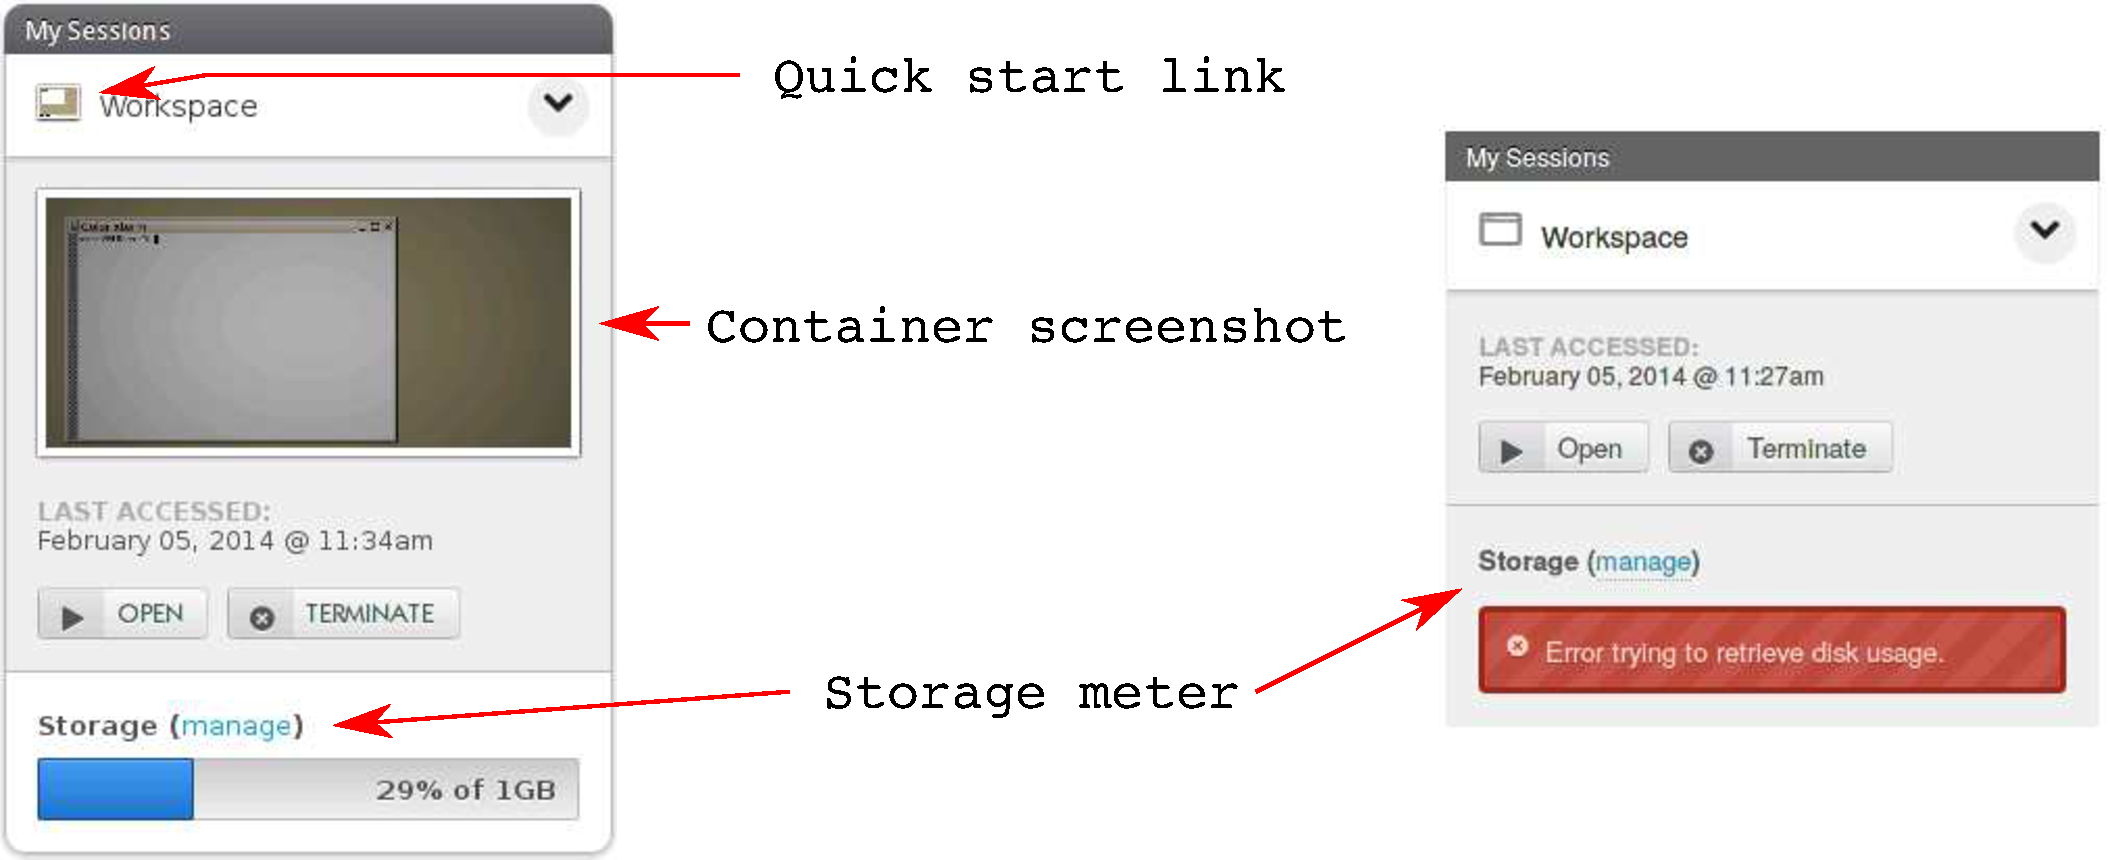
\includegraphics[width=0.98\textwidth]
    {../../images/eps/hub+configuration+dashboard+my+sessions+2.pdf}
  \caption{ The \texttt{My Sessions} module can be configured to show
            screen shots of the tool session containers, provide short
            cut links to access the container, and display the user's
            available disk storage on the hub. The module on the left
            is fully configured showing the container screenshot, an
            enabled quick start link, and storage meter. The module
            on the right has some of these features disabled.}
  \label{fig:my_sessions_module_compare}
\end{figure}


The My Sessions module can be configured to provide the user with a shortcut
link to access active tool session containers and screen shots of applications
running inside of an active tool session container.  Capturing screen shots of
the tool session container is a function performed by the middleware and is not
available in the open source release prior to version 1.2.1. Because of this,
the feature is turned off by default. Hosted hubs, managed by the HUBzero Team,
run an advanced version of the middleware that supports this feature. When new
hosted hubs are launched, turning this feature on is often missed.

Similarly, the availability of the disk usage and quota information depends
upon the hub being configured to show the information and having the
\xfprogramname{telequotad}
% FIXME: should probably cite hubzero-telequotad
service running on the hub's fileserver. When the hub is not configured to show
the disk usage, or the telequotad service is not running, users are shown
messages like those in the image on the right side of
\Cref{fig:my_sessions_module_compare}, explaining that the information is
unavailable or simply stating the used disk space is \textbf{0\% of 0GB} when
the user has no quota set.

When a hub is first installed, there are many settings that can be adjusted to
change the user experience. HUBcheck provides a library to help developers
automate the validation of these settings through the hub's website, from the
user's perspective. Using HUBcheck, developers can write automation scripts
that can login to the hub website as a user, start a tool session container,
and test if the My Sessions module is correctly showing screen shots and
enabling short cut links.


%\begin{enumerate}
%\item login to the hub website as a user
%\item navigate to the user's Dashboard web page
%\item launch a new tool session container
%\item navigate back to the user's Dashboard web page
%\item verify that the new tool session container is
%      listed in the My Sessions module
%\item verify that the tool session container's entry
%      in the My Sessions module contains a shortcut link
%      to open the tool session container.
%\item verify that the tool session container's entry
%      in the My Sessions module contains a screen shot
%      of the tool session container.
%\end{enumerate}


%\begin{figure}[ht!]
%  \centering
%  \includegraphics[width=0.5\textwidth]
%    {../../images/catalyzecare_dashboard_my_sessions_no_screenshot_shortcuts.png}
%  \caption{ The \textit{My Sessions} module on the user's Dashboard shows
%            \textbf{0\% of 0GB} in the storage meter when the user has no
%            quota set. }
%  \label{fig:application_view_working_storage_meter}
%\end{figure}

%These two problems are easy to catch using an automated testing suite
%like HUBcheck. To find them, a HUBcheck test can be written to perform the
%following tasks:

Developers can also write HUBcheck based automation scripts to identify
problems like the improper disk usage calculation mentioned earlier. To do this
by hand a developer would:

\begin{figure}[H]
  \vspace{-10pt}
  \begin{minipage}[c]{0.48\linewidth}
    \begin{enumerate}
    \item login to the hub website as a user;
    \item navigate to the user's Dashboard web page;
    \item locate and read the disk storage string from the web page;
    \item validate the string holds the proper format.
    \end{enumerate}
  \end{minipage}
  \hfill
  \begin{minipage}[c]{0.48\linewidth}
    \centering
    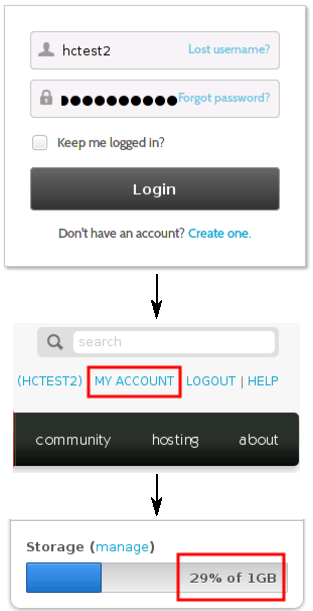
\includegraphics[scale=0.7]
      {../../images/eps/check+user+storage+meter+process+2.pdf}
%    \caption{Process to check that the user's storage meter is being displayed.}
    \caption{Accessing user's storage meter.}
    \label{fig:check_user_storage_meter_process}
  \end{minipage}
\end{figure}


The HUBcheck script shown in
\Cref{lst:dashboard_mysessions_check_storage} follows the same steps.  The
format of the disk storage string should match the format similar to
\textbf{X\% of YGB}, where X is an integer, ranging from 0 to 100, describing
the percentage of the user's available disk that has been used, and Y is a
positive integer describing the amount of disk space available to the user, in
gigabytes.

HUBcheck's web automation library simplifies common tasks like logging into the
hub website and navigating to web pages. The library also provides abstractions
of hub web pages, called page objects, so developers can reuse common blocks of
code and take advantage of a standard library for locating elements on the web
page.


\begin{xcode}{%
  language=Python,%
  label=lst:dashboard_mysessions_check_storage,%
  caption={Checking user's storage meter, using a HUBcheck backed script} %
}
...
# launch the browser and navigate to hub website
hc.browser.get('https://hubzero.org')

# login to the hub website as a user
hc.utils.account.login_as(username,userpass)

# navigate to the user's Dashboard web page
po = hc.catalog.load_pageobject('GenericPage')
po.header.goto_myaccount()

# locate and read the disk storage string from the web page
po = hc.catalog.load_pageobject('MembersDashboardPage')
storage_amount = po.modules.my_sessions.storage.storage_meter()

# validate the string holds the proper format
assert storage_amount != '', 'invalid storage amount returned'
assert storage_amount != '0% of 0GB', 'user quotas not activated'
...
\end{xcode}


\section{Hub Upgrade Issues}
\label{sec:problem_upgrade}

Errors also tend to arise on the hub after software upgrades.  These types of
errors can usually be traced back to configuration changes in upgraded hub
modules, the release of errant software, or pre-existing errors on the upgraded
hub that manifest themselves after the upgrade. Running HUBcheck after a hub
has been upgraded can help identify errors related to hub upgrades before the
user experiences them.

\begin{figure}[ht]
  \centering
  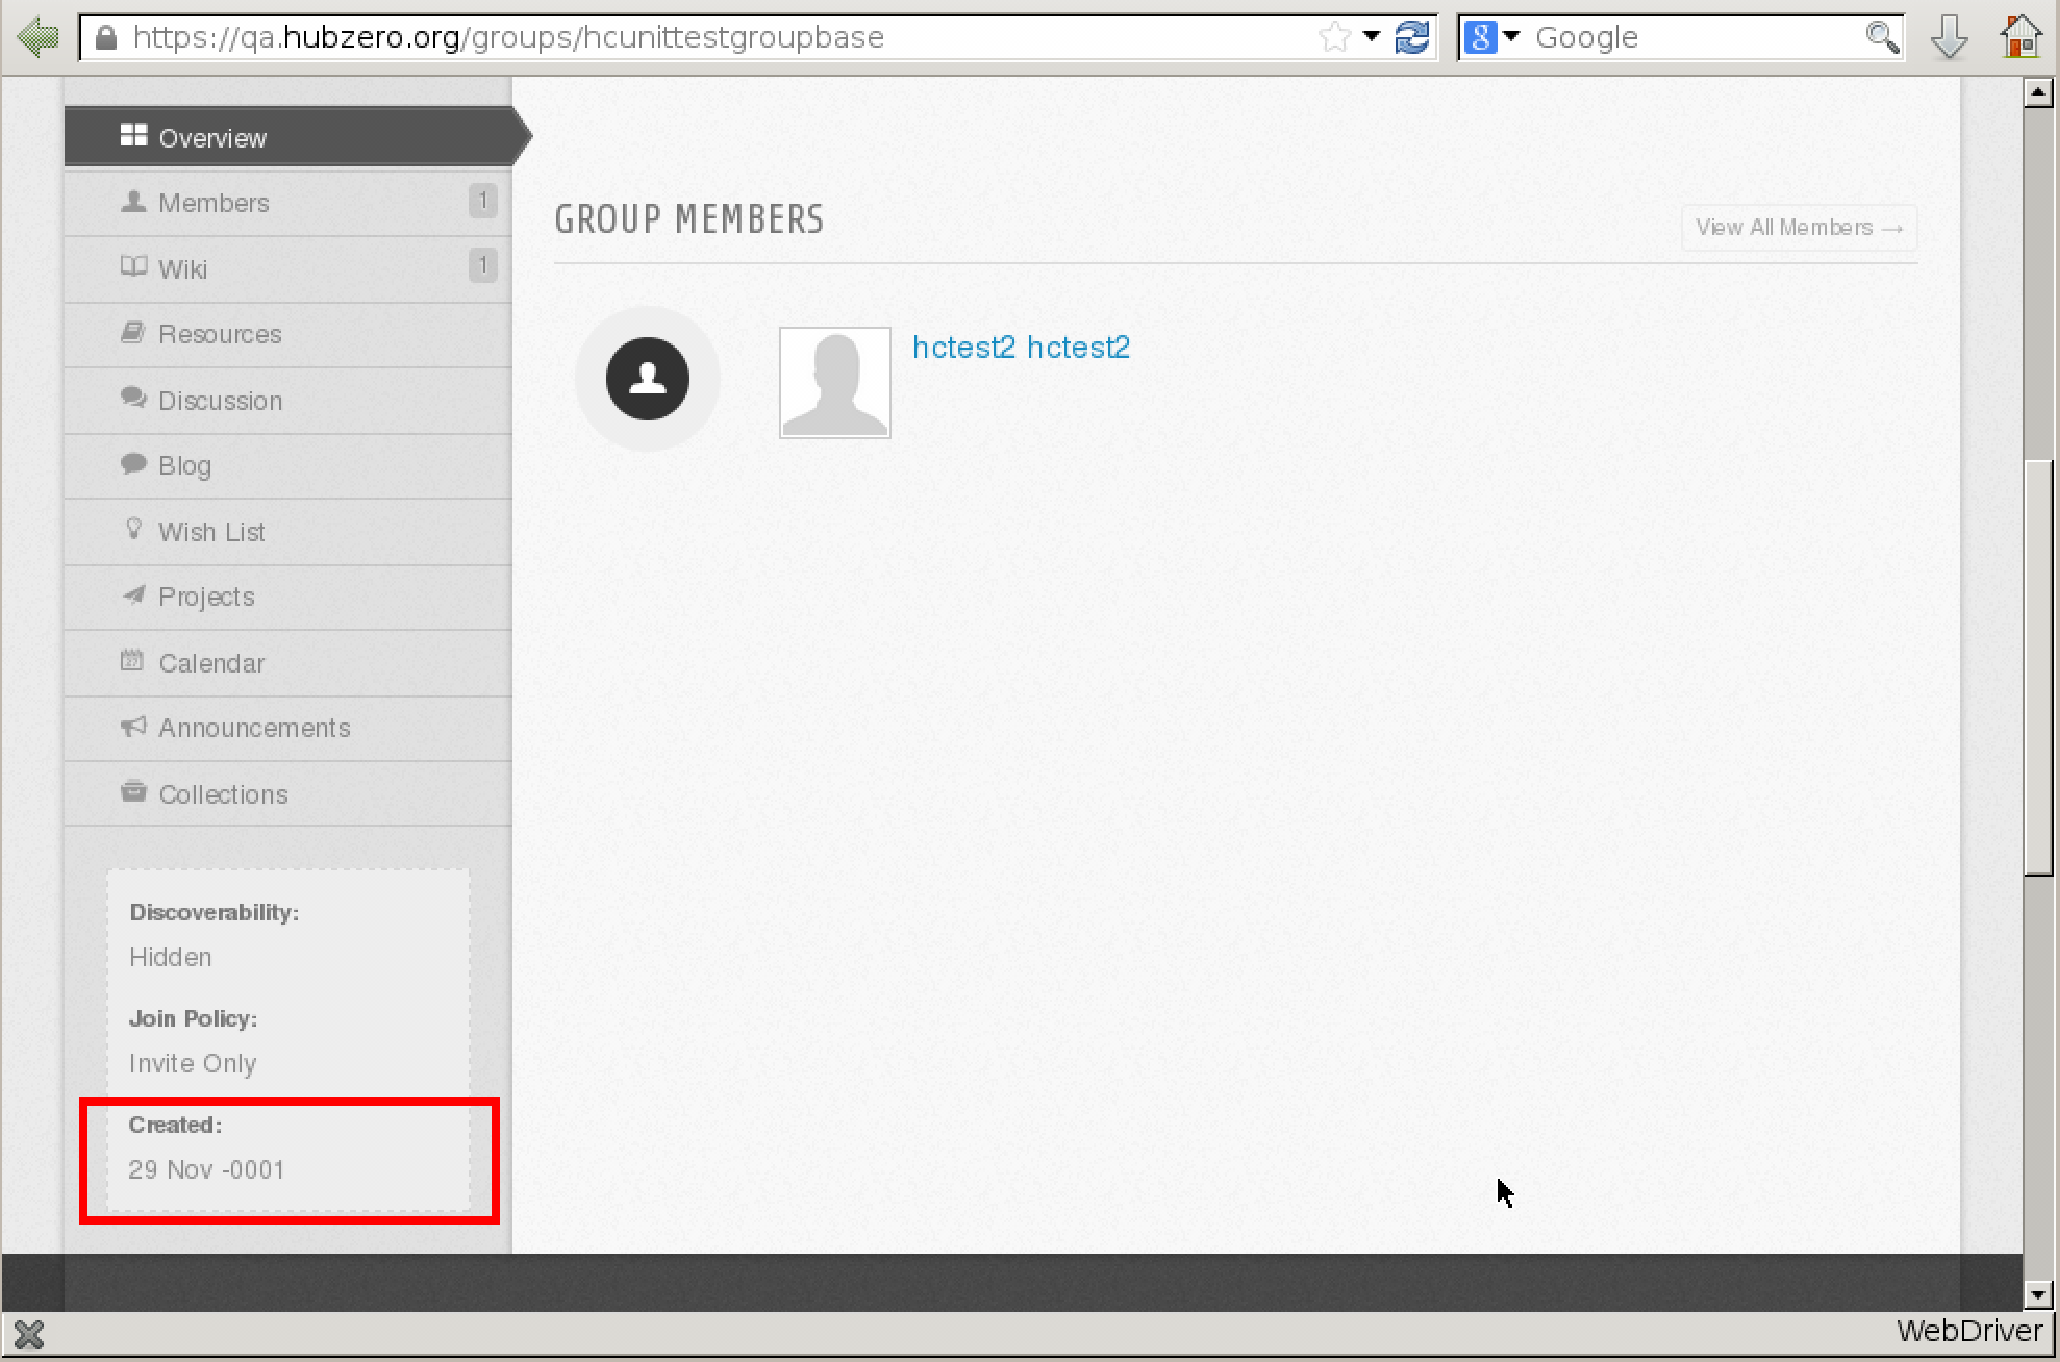
\includegraphics[width=0.5\textwidth]
    {../../images/eps/qahubzero_v1_2_group_create_date_bad_year.pdf}
  \caption{ Sometimes errors show up after a hub upgrade like this one, where
            the create date of a new hub group was not being displayed correctly.
            Finding this type of bug is tedious for a human, but developers
            can use HUBcheck to write tests which verify that multistep processes,
            like creating a group, still produce expected results.}
  \label{fig:group_create_date_bad_year}
\end{figure}


One example of a hub upgrade related error that HUBcheck was able to identify
occurred in the hub's \texttt{Groups} component. The \texttt{Groups} component
allows users to organize content and discussions within the hub community. The
component provides discussion forums, wiki pages, blogs, project spaces and
more. Users can create a group by filling out a web form on the hub website.
Groups on the hub have an overview web page that provides some properties of
the group like group name, description, number of members, join policy and
create date.

In this case, HUBcheck was run on a test hub after a software upgrade. A
failing test alerted developers to an error in displaying the create date for
newly created groups.  With knowledge of the problem, hub developers were able
to identify and fix the the errant code before it was propagated to more
hubs, which would have resulted in additional cleanup work.

To find this type of error, a new group needed to be created on the hub, and
its properties verified. The process of creating and verifying a new group on
the hub can be tedious and error prone for a human, but with HUBcheck it can be
done in a few lines of code in a testing script.


\section{Hub Reboot Issues}
\label{sec:problem_reboot}

When the servers hosting a hub are shut down and brought back up, it is easy
for unexpected problems to arise. From hosts having trouble rebooting to remote
filesystems not being properly mounted over the network, machine reboots are a
time where errors can happen that leave the hub not living up to its fullest
potential.  Developers can exercise hub functions quickly by running HUBcheck
after a reboot. HUBcheck provides the type of automation primitives that
encourage developers to tackle the harder problems to automate, like checking
that render servers are accepting connections from within a tool session
container.

\begin{figure}[]
  \centering
  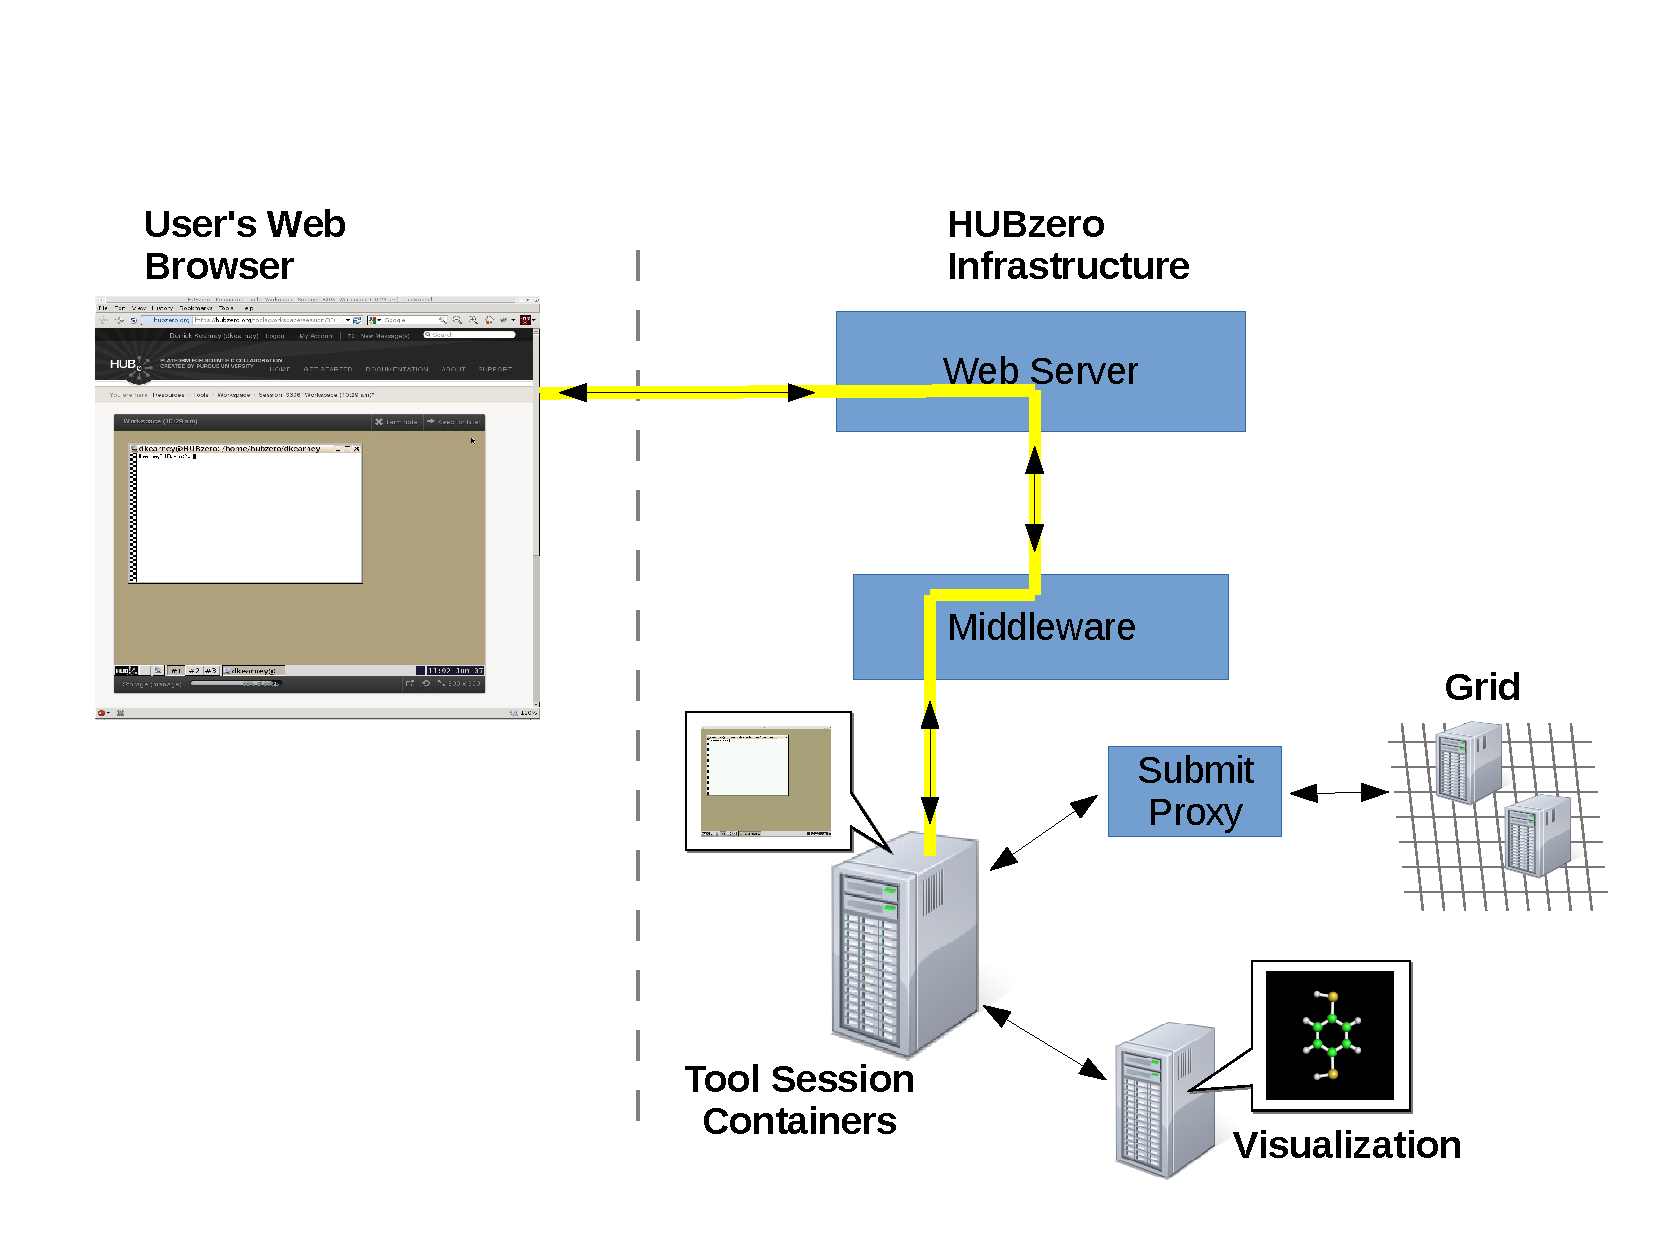
\includegraphics[width=\textwidth]
    {../../images/hubcheck_block_diagram/tool_session_container_block.pdf}
  \caption{ Simulation tool developers use a tool session container to
            develop and deploy their work on the hub. Checking that the
            containers are properly configured is time consuming for a
            human because of the layers of software between the web
            browser and the container's services like Submit and the
            Visualization servers.}
  \label{fig:tool_session_container_block_diagram}
\end{figure}

One of the key features of a hub is its ability to run interactive simulation
tools that are displayed in the user's web browser. These simulation tools are
run in an environment called a tool session container on an execution host that
is a part of the hub. In their web browser, the user sees a display of the tool
session container that has been projected to them, from the hub, using the VNC
protocol. Hosting the interactive simulation tools on the hub allows the user
to take advantage of many features that would not normally be found on their
own system, like access to grid computing services and powerful rendering
machines for interactive visualization.

The tool session container is a Debian Linux environment that supports the
building of simulation tools by tool content developers and the execution of
tools by hub users. Access to grid computing and render machines are services
provided to the tool session containers. After a reboot of the hub these
services should be restored, and if they are not, the simulation tools may not
work correctly.

There are two ways to access a tool session container. The most frequently used
way is through the web browser. Starting a tool on the hub gets the user access
to a tool session container. This approach doesn't allow the user to automate
interaction in a terminal with a shell. The second way is to connect over SSH,
the secure shell protocol. All tool developers can access a tool session
container in this way. This approach has the advantage that it gives access to
a terminal with a shell, and shell automation tools like Expect
\cite{libes1995exploring} have existed since the mid 1990s.

HUBcheck takes advantage of this second approach to accessing a tool session
container and provides a small, Expect-like, shell automation library. Using
HUBcheck, hub developers can write automation scripts that enter a tool session
container and examine the resources that are supposed to be available for tools
to use, like access to the render servers. They can also write scripts to check
if a render server is accepting connections from within the tool session
container, examine the container firewall setup, installation of software such
as the Rappture Toolkit, access to grid infrastructures through the
use of the \xfprogramname{submit} command, file transfer between the user's desktop
and the user's hub account using the \xfurischeme{sftp}, \xfurischeme{filexfer}, or
\xfurischeme{webDAV} protocols, and simulation tool invocation through
\xfprogramname{invoke\_app}, all under the same conditions a simulation tool would be
making its request from.


\section{Multimodal System Automation}
\label{sec:problem_automation}


HUBcheck's combination of web and shell automation libraries helps it provide
developers with the unique ability to write scripts that capture the user
experience of working in the dual environment system that is the hub. While a
great deal of testing and automation can be performed by libraries that only
access the website, or only access the tool session container, there exists a
set of tasks whose operations span both the website and the tool session
container, that no other single tool can automate. These are the cases of a
growing area of interest within the hub, where information is passed from
resources published on the website to tools running inside of the tool session
container. In hub parlance, this is referred to as \textbf{parameter passing}.

Simulation tools run in a tool session container, either on the same host as
the hub's web server or on a separate execution host. While this approach has
its advantages with respect to deploying tools in a consistent environment --
isolation between different users running tools and isolation between tools and
the web server -- there are also a number of disadvantages, one of which is the
inability to easily pass parameters to the simulation tool before it has
launched.

Launching a simulation tool on the hub involves coordination between both the
hub website and hub middleware. It can be explained in five steps and are shown
in \Cref{fig:start_tool_session_container_diagram}:

\begin{enumerate}
\item User click's link to launch tool from web page.
\item Web link calls PHP function which forwards request to middleware.
\item Middleware starts a new tool session container for the tool.
\item Middleware calls the tool's invoke script inside of the tool session container.
\item Invoke script execs command to start tool's graphical user interface.
\end{enumerate}

\begin{figure}[ht]
  \centering
  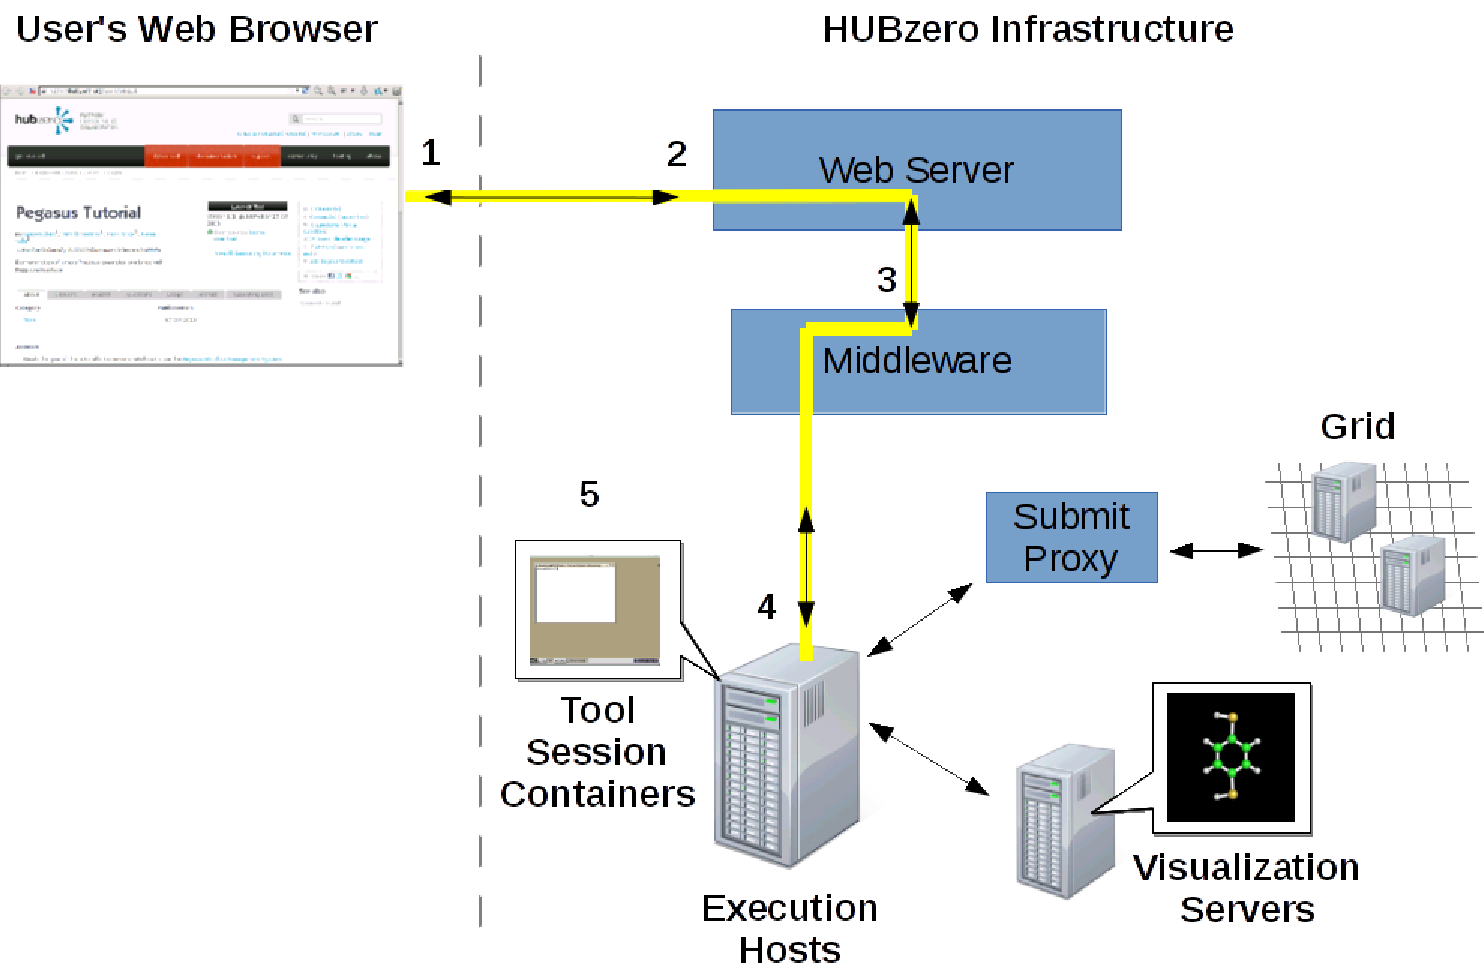
\includegraphics[width=\textwidth]
    {../../images/eps/start+tool+session+container+diagram2.pdf}
  \caption{ Simulation tools are started by user's clicking a link on the hub
            website. The link forwards the request to the middleware, which
            handles allocating a tool session container and calling the tool's
            invoke script. The invoke script sets up the environment for the
            tool to run in, and finally, launches the tool.}
  \label{fig:start_tool_session_container_diagram}
\end{figure}

There are a couple of ways to start the process to launch a simulation tool on
the hub. The most obvious way is to use a web browser to navigate to the tool's
\textit{tool information page}, a web page that describes what the tool does,
lists its authors and funding sources, and includes a link to launch the tool.
In the first step, the user navigates to the tool information page and clicks
the link to launch the tool.  Clicking the web link sends a request to the hub
web server asking it to start the tool. The hub web server receives the request
and calls upon the hub middleware to launch the new tool.  In step three, the
middleware supplies a tool session container to run the requested tool.

Tools published on the hub include an \textit{invoke script} which contains all
of the commands necessary to launch the simulation tool, including setting up
system environment variables with prerequisite library and executable paths.
In step four above, the middleware enters the tool session container as the
user, and execs the tool's invoke script to start the graphical user interface.
Lastly, the invoke script sets environment variables for the libraries needed
by the tool and launches the tool.

Version 1.2 of the HUBzero software included new components that allowed users
to interact with learning concepts and data through the use of simulation and
modeling. Two examples of this include the Databases component and the Courses
component. The Databases component allows users to create databases of
information and construct views that help others understand their data. The
Courses component allows teachers to manage an online class, hosted on the hub,
that incorporates hub resources including simulation tools.  With both of these
components, developers may want to pass data that is stored on the hub website
over to a tool running in a tool session container.

To address this need, a new algorithm for allowing parameters to be passed from
the website into a simulation tool running in a tool session container was
created. The algorithm accepts a limited number of data types (file names,
directory names, and integers) and encodes the parameters into the URL used to
launch the tool. The parameters are passed through the hub web server and
middleware, which have the opportunity to check them for validity, and into the
tool session container. Once inside of the tool session container, they are
stored in a file, and the tool developer is responsible for parsing them out of
the file, either through the tool's invoke script, or in the simulation tool
itself.

Whether it is data from a database being fed into a cancer prediction model, or
example parameters for simulating a circuit from a class, passing data between
the website and the tool session container involves many layers of software
that have the opportunity to manipulate or lose the data. Passing data is
difficult to do and tedious to test.  HUBcheck provides the automation
primitives necessary to ease the task of writing scripts that can interact with
the website and tool session container in the same script. In the case of
parameter passing, hub developers were able to use HUBcheck's web and shell
automation libraries to build a test suite to exercise passing parameters to a
simulation tool by crafting both valid and invalid URLs. As a part of the test
suite, numerous simulation tools were installed on the hub and URLs were
generated to match the requirements and restrictions of the parameter passing
algorithm. After launching tools with the specialized URLs, the HUBcheck based
scripts accessed the tool session container running the simulation tool and
verified that the parameters were passed through the tool invocation labyrinth
(which includes the web browser, web server, middleware, and tool session
container), through the tool's invoke script, and to the tool where they could
be processed.



% talk about the external libraries that hubcheck depends upon.
% selenium webdriver
% browsermob proxy
% paramiko
%
%  hubcheck.tex  2012-04-09  Derrick Kearney
%
%  Describe what hubcheck is and the pieces that make it up.
%

%\setenumerate[1]{label=\Roman*.}
%\setenumerate[2]{label=\Alph*.}
%\setenumerate[3]{label=\roman*.}
%\setenumerate[4]{label=\alph*.}
%\begin{outline}[enumerate]

%\1 Selenium WebDriver
%  \2 Abstracts web browser automation.
%  \2 Focused on reproducing how a user interacts with the web page.
%  \2 Support actions like clicking on element, typing in inputs, moving
%     the mouse pointer.
%  \2 Relies on web browser to execute javascript.
%  \2 Works with Firefox, Opera, IE, PhantomJs, Safari, Mobile browsers, others.
%  \2 Runs in remote server mode or local mode.
%  \2 Controls starting a new web browser for each test case.
%  \2 User can send commands to browser using Java or other languages
%     through a RESTful, JSON based, remote wire protocol web service.
%  \2 Results of commands are sent back to user, through the programming language,
%     for processing.
%\1 BrowserMob Proxy
%  \2 Built to capture performance data for web applications
%  \2 Can be used to record, redirect, and block http and https requests.
%  \2 Records HTTP Archive (HAR) which provides HTTP status codes,
%     along with request/response timings among other things.
%  \2 Provides information about requests that are not provided by
%     Selenium WebDriver. Selenium WebDriver wants to stay focused
%     on user interactions.
%\1 Paramiko
%  \2 Python module that implements the SSH version 2 protocol
%  \2 Allows for creating SSH and SFTP connections for secure connections
%     to remote machines.

\chapter{EXTERNAL LIBRARIES}
\label{chap:external_libraries}

HUBcheck builds upon several external libraries to provide web browser and
shell based automation. To support web automation, HUBcheck uses the Selenium
WebDriver API \cite{SeleniumWebDriver:Online} and the BrowserMob Proxy
\cite{BrowserMOBProxy:Online}. The WebDriver API is used to control the web
browser and is provided by the Selenium project along with bindings for several
programming languages. The BrowserMob Proxy is an open source web proxy,
maintained by Patrick Lightbody, which can be used to watch and manipulate
network traffic. To support shell automation, HUBcheck builds upon Paramiko
\cite{Paramiko:Online}, a Python implementation of the SSH version 2 protocol.
Below we'll learn more about the role each of these libraries plays.

\section{Selenium WebDriver}
\label{sec:external_libs_selenium}

% describes the webdriver api
% http://www.w3.org/TR/webdriver/

% describes the firefox driver
% http://code.google.com/p/selenium/wiki/FirefoxDriver

Selenium is an open source project with a suite of tools used to automate web
browsers across many platforms. Selenium implements the WebDriver API as a part
of the Selenium WebDriver library. The WebDriver API provides an
object-oriented programming interface to communicate with and control a web
browser, performing the same actions a person would when interacting with a web
page.  Through the WebDriver API, developers can launch a web browser, locate
elements in web pages, and perform actions on elements such as typing into them
or clicking on them using the mouse. The following subsections show examples of
how Selenium WebDriver can be used to control a Firefox web browser using the
Python programming language.

\subsection{Launching a Web Browser}
\label{ssec:external_libs_selenium_launch_browser}

The Selenium WebDriver Python bindings provide the \xfmodule{webdriver}
module that holds classes to represent the different types of browsers that
can be launched, including Firefox, Chrome, Safari, Opera, and PhantomJS.
Browsers can be launched locally on the same machine running the automation
program, or on a remote host that is running a Selenium Server. Each browser
has a special plugin which translates the WebDriver requests,
made from Selenium, to the browser's native automation API.

Launching a web browser using Selenium is as simple as instantiating a new
\xfobject{webdriver} object for the browser the user wants to launch. With no
initialization arguments, the user will be provided with a new browser they can
control by calling member functions of the returned object as demonstrated in
\Cref{lst:selenium_launch_browser}.


\begin{xcode}{%
  language=Python,%
  label=lst:selenium_launch_browser,%
  caption={Launching a locally hosted Firefox web browser using Selenium WebDriver's Python API},%
}
from selenium import webdriver

browser = webdriver.Firefox()
browser.get('https://hubzero.org')
\end{xcode}


%Properties of the web browser and desired system to host the browser can be
%passed to the driver. This is useful when automating in an environment where
%multiple web browsers or host systems are available. Browser capabilities
%include items like the host platform, file paths to browsers, and
%expressing operating system requirements. \Cref{fig:capabilities_setup}
%shows how to setup a capabilities dictionary to start the Firefox browser on a
%Debian/Linux system using the Python programming language.
%
%\begin{xcode}{%
%  language=Python,%
%  label=lst:capabilities_setup,%
%  caption={The capabilities dictionary is used to tell the driver program what system properties are desired for the browser that is about to be launched.}%
%}
%capabilities = {}
%capabilities['platform'] = 'ANY'
%capabilities['browserName'] = 'firefox'
%capabilities['version'] = ''
%capabilities['javascriptEnabled'] = True
%capabilities['firefox\_binary'] = '/usr/bin/firefox'
%\end{xcode}


For some browsers, more fine grained web browser controls are exposed to the
developer through access to the browser's profile.  Not all browsers support the
profile concept. Firefox allows users to load a pre-configured profile or
create one on the fly.

\begin{xcode}{%
  language=Python,%
  label=lst:firefox_profile_example,%
  caption={Adjusting the preferences in the Firefox browser.}%
}
from selenium import webdriver

profile = webdriver.FirefoxProfile()
profile.set_preference('browser.startup.page',0)
profile.set_preference('app.update.enabled','False')
profile.add_extension('firebug-1.11.4.xpi')
profile.set_preference('extensions.firebug.currentVersion','1.11.4')

browser = webdriver.Firefox(firefox_profile=profile)
browser.get('https://hubzero.org')
\end{xcode}

\Cref{lst:firefox_profile_example} demonstrates setting up a Firefox
browser profile that disables the startup page, disables automatic updates to
the browser, and installs the Firebug browser extension.  The FirefoxProfile
class allows developers to set preferences and add extensions to the Firefox
browser. Alternatively, users can take advantage of the class's
\xfparameter{profile\_directory} argument to load a pre-configured browser
profile.

The \xfclass{webdriver.Firefox} class is used to launch the web browser. If a
custom profile was created it can be provided to the class and a web browser
based on those settings will be started. The object returned, shown in line 9
of \Cref{lst:firefox_profile_example}, is stored in the variable
\xfparameter{browser}, and is used in automation scripts as the object
reference for the web browser. All commands to the web browser, such as
navigation and locating web elements in the HTML DOM (Document Object Model),
are performed on the \xfparameter{browser} variable using the \xfmethod{get()}
and \xfmethod{find\_element()} family of methods.

\subsection{Locating Elements on the Web Page}
\label{ssec:external_libs_selenium_locating_elements}

%The first step to doing anything interesting with a web page is to be able to
%locate HTML elements on the web page. The \textit{browser} object provides 6
%variations of the \textit{find\_elements()} method to help the user located
%HTML elements. Each variation allows the automation developer to use a
%different strategy for locating the elements.

To perform actions on elements of a web page, Selenium must first be able to
locate the elements. Web element \textit{locators} are used by Selenium commands to
identify elements on a web page.  There are several different strategies for
locating web page elements listed in \Cref{tab:locatorMethods}. Two of the
most popular strategies are XPath expressions and CSS selectors.

\begin{table}[h]
  \centering
  \caption{Selenium element locator methods provide a variety of ways to find
elements on a web page.}
  \begin{tabular}{ | c | p{5cm} | c | }
    \hline
    Locator Strategy  & Description           & Example Use \\
    \hline
    id                & Search for a web
                        element with an id
                        attribute matching
                        the argument.         & id=username \\
    \hline
    name              & Search for a web
                        element with a
                        name attribute
                        matching the
                        argument.             & name=username \\
    \hline
    XPath             & Search for a web
                        element using
                        an XPath expression.  & xpath=//input[@id='username'] \\
    \hline
    link              & Search for a link
                        (anchor web element)
                        with text matching
                        the provided pattern. & link=link text \\
    \hline
    CSS               & Search for a web
                        element using a
                        CSS style selector.   & css=input\#username \\
    \hline
  \end{tabular}
  \label{tab:locatorMethods}
\end{table}

There is typically overlap in how the different locator strategies can be used
to locate elements on a web page. It is not uncommon for a single web element
to be identifiable by two or three of the locator strategies, but the key to
building robust automation scripts is to choose the most robust locator that
will withstand updates to the web page layout.

%\begin{xcode}{%
%  language=html,%
%  label=fig:hubzero_login_page_username_html,%
%  caption={The username input text box from the https://hubzero.org/login web %
%            page can be identified by several different element attributes    %
%            including by name, id, type, or class. XPath expressions or CSS   %
%            selectors can be written for using any of these attributes}%
%}
%<label>
%    Username:
%    <input id="username" class="inputbox" type="text" name="username">
%<\label>
%\end{xcode}


\begin{figure}[H]
  \begin{minipage}[c]{0.48\linewidth}
    \begin{xcode}{%
      language=html,%
      label=lst:hubzero_login_page_username_html,%
      caption={HTML for username field}%
    }
    <label>
        Username:
        <input id="username" class="inputbox" type="text" name="username">
    <\label>
    \end{xcode}
  \end{minipage}
  \hfill
  \begin{minipage}[c]{0.48\linewidth}
    \centering
%    \includegraphics[scale=0.6]
    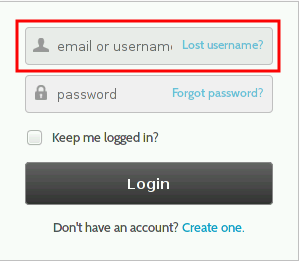
\includegraphics[width=0.8\textwidth]
      {../../images/eps/hubzero_login_page_username_field.png}
    \caption{Hub login form.}
    \label{fig:hubzero_login_page_username_html_2}
  \end{minipage}
\end{figure}

Take, for example, the hub login form shown in
\Cref{fig:hubzero_login_page_username_html_2}. The form contains a number of web
elements we would like to interact with, the most important of which are the
username field, password field, and login button.
\Cref{lst:hubzero_login_page_username_html} shows the HTML representation of the
username element in the login form.

Several of the locating strategies in Selenium can be used to identify the
element.  The examples in \Cref{tab:locatorMethods} show how this would be
done.  Among the available strategies, the ones involving the \xfparameter{id}
attribute are generally the most robust because HTML requires that the
id attribute be unique for all elements. This ensures that if the id attribute
exists for an element in the HTML DOM, then it should only exist once, reducing
the number of false positives when locating elements.

The locating strategies map directly to the Selenium WebDriver API functions
used to locate elements on the web page from a program. For the Python
bindings, these are a part of the \xfmethod{find\_element\_by\_*()} family of
methods shown in \Cref{lst:selenium_webdriver_find_element_functions}
Any one of these methods can be used to locate elements on a web page.

\begin{xcode}{%
  language=Python,%
  label=lst:selenium_webdriver_find_element_functions,%
  caption={The find\_elements\_by\_*() functions locate %
            web elements in Python.}%
}
# locating elements by the id attribute
element = browser.find_element_by_id('username')

# locating elements by name attribute
element = browser.find_element_by_name('username')

# locating elements by tag name
element = browser.find_element_by_tag_name('input')

# locating elements by XPath
element = browser.find_element_by_xpath("//input[@id='username']")

# locating elements by CSS Selector
element = browser.find_element_by_css_selector('input#username')
\end{xcode}

\subsection{Performing Actions on Web Elements}
\label{ssec:external_libs_selenium_performing_actions}

Once an element has been located, an action can be performed on the element.
Common actions include clicking on the element, sending key strokes to the
element, reading the properties of the element, and checking if the element is
displayed. \Cref{lst:selenium_webdriver_perform_actions_on_element}
demonstrates performing actions on the username field of the login web page.
In line 2, the username field is located using a CSS selector element locating
strategy. Lines 8 - 10 show that elements can be brought into focus on the web
page with the \xfmethod{click()} method, have its value erased using the
\xfmethod{clear()} method, and a new value assigned using the
\xfmethod{send\_keys()} method. By the end of this program, the username field on
the login page would be populated with the name ``hctest''.

\begin{xcode}{%
  language=Python,%
  label=lst:selenium_webdriver_perform_actions_on_element,%
  caption={Filling in the username field on the login form}%
}
# locate the username field by CSS Selector
element = browser.find_element_by_css('input#username')

# perform actions on the element:
# click the field to set focus
# clear any previous value from the field
# send key strokes to the field to fill in the username
element.click()
element.clear()
element.send_keys('hctest')
\end{xcode}

\subsection{Performing Mouse Actions on Web Elements}
\label{ssec:external_libs_selenium_mouse_actions}

In addition to being able to perform normal actions on elements, Selenium
WebDriver allows automation developers to perform mouse actions on elements
with a feature called ActionChains. ActionChains are useful for automating
tasks where a mouse movement is needed to trigger a property change in an
element on the web page. A common examples of this include JavaScript based
menus that appear on the screen when the mouse hovers over an element on the
web page, as shown in \Cref{fig:user_account_menu_closed}.

Selenium tries hard to only allow interaction with visible page elements that a
user would be able to interact with. If an element is present on the web page
and is available in the HTML DOM that the browser loaded, but is not visible to
the user, Selenium will not allow the automation code to perform actions on it.
Properties, like the text of the element or the attributes of its HTML, can
still be read, but clicking on the element or sending key strokes to the
element will fail.

To emulate the movement of the mouse, the automation developer can use Selenium
WebDriver's ActionChains.  ActionChains allow the automation developer to
specify elements on the web page to perform mouse actions on. ActionChains
support hovering the mouse over elements, single clicking elements, double
clicking elements, context (right) clicking elements, clicking and dragging
elements, and pressing a number of meta (ctrl, alt, shift) key combinations in
coordination with a mouse action.

\begin{figure}[htb]
        \centering
        \begin{subfigure}[b]{0.48\linewidth}
                \centering
%                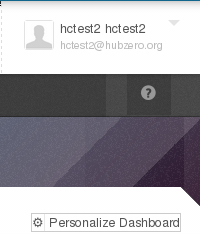
\includegraphics[width=0.5\textwidth]{../../images/corehubzero_javascripty_account_menu_closed.png}
                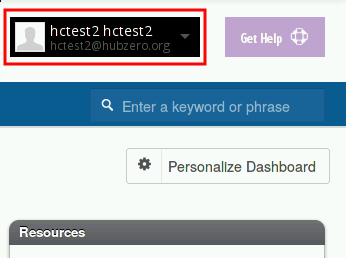
\includegraphics[width=\linewidth]{../../images/eps/nciphub_user_account_menu_closed.png}
                \caption{User account menu closed.}
                \label{fig:user_account_menu_closed}
        \end{subfigure}
        \begin{subfigure}[b]{0.48\linewidth}
                \centering
%                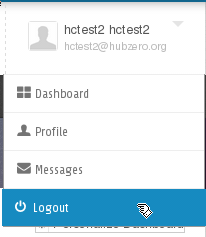
\includegraphics[width=0.5\textwidth]{../../images/corehubzero_javascripty_account_menu_open.png}
                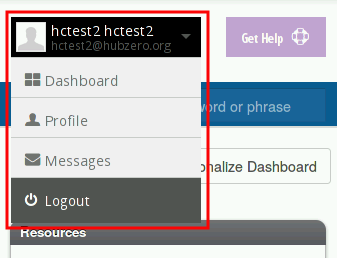
\includegraphics[width=\linewidth]{../../images/eps/nciphub_user_account_menu_open.png}
                \caption{User account menu open.}
                \label{fig:user_account_menu_open}
        \end{subfigure}
        \caption{Selenium WebDriver provides ActionChains to automate
                 performing mouse actions on elements of a web page.
                 ActionChains can be used for things like right or
                 left clicking on an element, drag and drop, and
                 hovering the mouse over an element.}
        \label{fig:action_chains_javascript_logout}
\end{figure}

On the hub, performing mouse actions is handy when trying to interact with the
user account menu, which requires the user to hover the mouse over the menu
element, shown in \Cref{fig:user_account_menu_closed}, in order to expose
account navigation options that lead to the user's Dashboard, Profile,
Messages, or log the user out of the website. To do this programmatically using
the Python bindings, an automation script would use the
\xfmodule{action\_chains} module.

\begin{xcode}{%
  language=Python,%
  label=lst:action_chains_javascript_logout_code,%
  caption={Activating a JavaScript menu using ActionChains.}%
}
# load the ActionChains class
from selenium.webdriver.common.action_chains import ActionChains

# locate the menu and logout elements by CSS Selector
menu_element = browser.find_element_by_css('#account')
logout_element = browser.find_element_by_css('#account-logout')

# build the ActionChains object to perform a mouse action:
# move the mouse over the menu to activate the JavaScript menu
# move the mouse to the logout list item in the menu
# single click the logout menu item
actionProvider = ActionChains(browser)
actionProvider.move_to_element(menu_element)
actionProvider.move_to_element(logout_element)
actionProvider.click()
actionProvider.perform()
\end{xcode}

Developers use the \xfclass{ActionChains} class to build (chain) a list of
actions together and send them to the web browser to be performed as if they
came from the computer's mouse.
\Cref{lst:action_chains_javascript_logout_code} demonstrates this by providing
a solution to the problem of hovering the mouse over the menu in
\Cref{fig:user_account_menu_closed}, exposing the account navigation options
shown in \Cref{fig:user_account_menu_open}. More specifically, the script
focuses on clicking the \xfhtmllink{Logout} link in the menu.

As with most Selenium WebDriver related scripting tasks, the first step is to
locate the web elements items the script will be interacting with in the HTML
DOM. Lines 5 and 6 of \Cref{lst:action_chains_javascript_logout_code}
are responsible for locating the menu element and the logout link on the web
page. Next, in lines 12 through 15, the script builds up a list of commands that
should be performed by the mouse. Each line in the script adds another command
that should be performed to the list stored in the variable
\xfparameter{actionProvider}. To get to the logout link, the mouse must first move
to the menu element, line 13, then move to the logout element, line 14, and
lastly send a click signal to press the logout link, line 15. The commands are
stored until the developer asks for them to be performed, shown in line 16 of
the script.


\subsection{Waiting for Web Elements}
\label{ssec:external_libs_selenium_waiting_for_elements}

% cite http://www.seleniumhq.org/docs/04_webdriver_advanced.jsp

Asynchronous JavaScript and XML (AJAX) is a programming technique that allows
web applications, running in the user's browser, to communicate with the web
server and dynamically change the state of the web application without
reloading the web page. The use of AJAX on web pages poses a problem for some
web automation software that evaluates static HTML DOMs without evaluating the
JavaScript that accompanies it.  After the browser makes a request for a web
page, the web server sends back a stream of HTML that can have JavaScript
embedded within it. The web browser is responsible for reading the HTML and
evaluating the JavaScript inside, which may request additional HTML from the
web server.

Selenium WebDriver uses the HTML and JavaScript engines inside of the external
web browser it is controlling to build the HTML DOM that represents the web
page the web browser loaded. This allows Selenium WebDriver to leverage the
same web browser to interpret and evaluate the HTML and JavaScript that a user
would.  This also adds a dimension of difficulty in locating web elements whose
presence or visibility on the web page is influenced by JavaScript. The dynamic
nature of JavaScript provides less structure to what it means for a web page to
have finished being `loaded'. Loading up multiple pieces of a web page may be
delayed, for example, by a slow network.  Selenium WebDriver provides two types
of waiting strategies, \textit{Implicit Waits} and \textit{Explicit Waits}, to
work around these unexpected delays and deal with locating elements that may
not be immediately available.

\subsubsection{Implicit Waits}
\label{sssec:external_libs_selenium_implicit_waits}

In Selenium WebDriver, the default behavior is to search once for a locator in
the HTML DOM.  If the locator cannot be found, a
\xfclass{NoSuchElementException} is raised. Implicit Waits are a way to
repeatedly search for a web element in the HTML DOM, while blocking other
commands from continuing, for a set amount of time before raising the
\xfclass{NoSuchElementException}.

Implicit waits can be setup once and exist for the life of the webdriver
object.  Setting up an implicit wait affects the whole family of
\xfmethod{find\_element*()} based methods, which will repeatedly search for the
element until either the element is found or the timeout limit is hit.

\subsubsection{Explicit Waits}
\label{sssec:external_libs_selenium_explicit_waits}

Explicit Waits consider the more general case where the automation developer
wants to wait for a condition to be met. Without explicit waits, many people
are tempted to check for the condition to be met while inside a \xfmethod{for}
loop, adding a call to the programming language's \xfmethod{sleep()} function
to space out the checks.  This approach should be avoided in favor of using the
\xfclass{WebdriverWait} class provided by the Selenium libraries.

% FIXME: add explicit wait example: submiting support ticket through the
%        need help interface.

\subsection{The Page Object Design Pattern}
\label{ssec:external_libs_selenium_page_objects}

The Page Object design pattern provides a layer of abstraction between a web
page and automation scripts. It represents the services offered on a web page
or a portion of a web page. By writing automation scripts that interact with
the page object, developers can significantly reduce the number of repeated
lines of code in their automation scripts, abstracting away many of the common
features of the code into a single class that needs to be updated as the web
page interface changes.

%Later on, we'll show how the use of the Page Objects design pattern helps
%reduce the size of the automation script, making it more readable, easier to
%write, and easier to maintain.


Novice developers learning to use Selenium for their web automation may start
by using the Selenium IDE, a graphical user interface product of the Selenium
project that records the actions of the user and stores them using an internal
representation called \textit{Selenese}. Selenium IDE also has the ability to
convert Selenese to a number of programming languages. The IDE allows
developers to quickly create automation scripts, but it suffers from the same
afflictions as manually writing automation scripts using the procedural
programming paradigm.  They both result in brittle scripts that break easily
and are painful to fix because of a lack of encapsulation.  With a little
organization and refactoring, these brittle scripts can be turned into robust
scripts that require less code to write and are easier to understand.

Consider the automation script in \Cref{lst:selenium_ide_hubzero_login},
which navigates the web browser to the \xfhtmllink{hubzero.org} web page,
clicks the link to login, then fills in the username field, fills in the
password field, and clicks the submit button.

\begin{xcode}{%
  language=Python,%
  label=lst:selenium_ide_hubzero_login,%
  caption={Simple hub login automation script.}%
}
from selenium import webdriver

# setup automation script constants
base_url = "http://hubzero.org/"

# start the browser
driver = webdriver.Firefox()

# navigate to the login page
driver.get(base_url)
driver.find_element_by_id("account-login").click()

# perform the login action
driver.find_element_by_css_selector("#username").clear()
driver.find_element_by_css_selector("#username").send_keys("abc")
driver.find_element_by_css_selector("#passwd").clear()
driver.find_element_by_css_selector("#passwd").send_keys("123")
driver.find_element_by_css_selector("[name='Submit']").click()
\end{xcode}


\noindent

Immediately looking at the code, a couple of patterns are apparent.  The first
pattern involves repeated searches for commonly used fields. This is true of
the field with id \xflocator{username}, which is searched for in line 14 to clear
it and again in line 15 to send it a value, and also for the the password field
with id \xflocator{passwd} for the same reasons in lines 16 and 17.  To clean up
this code, it could be rewritten to save the result of the first search to
a variable and call the \xfmethod{clear()} and \xfmethod{send\_keys()} methods on
that variable.

The second pattern involves the repeated steps used to populate a text field.
Every time a text field is populated, the script first searches for the
element, then clears the element of any previous value, and lastly, sends some
keys to the element. These actions could be combined into a function, as shown
in \Cref{lst:hubzero_login_utils} to help reduce the amount of repeated
code.

\begin{xcode}{%
  language=Python,%
  label=lst:hubzero_login_utils,%
  caption={populate\_input function included in utils.py}%
}
def populate_input(driver,loc,text):
  """type text into the element located by loc"""

  e = driver.find_element_by_css_selector(loc)
  e.clear()
  e.send_keys(text)
\end{xcode}

\noindent

An updated version of the automation script from
\Cref{lst:selenium_ide_hubzero_login} that addresses the first two patterns,
including a function named \xfmethod{populate\_input()} which finds an element
and types text into it, would look like this:

\begin{xcode}{%
  language=Python,%
  label=lst:hubzero_login_with_populate_input,%
  caption={Hub login script with repeated patterns abstracted away}%
}
from selenium import webdriver
from utils import populate_input

# setup automation script constants
base_url = "http://hubzero.org/"

# start the browser
driver = webdriver.Firefox()

# navigate to the login page
driver.get(base_url)
driver.find_element_by_css_selector("#account-login").click()

# perform the login action
populate_input(driver,"#username","abc")
populate_input(driver,"#passwd","123")
driver.find_element_by_css_selector("[name='Submit']").click()
\end{xcode}

At this point the automation script in
\Cref{lst:hubzero_login_with_populate_input} is looking pretty good. We were
able to abstract out most of the repeated code into a function,
\xfmethod{populate\_input()}, that we can pass arguments to and let it take
care of locating and writing text to elements of the HTML DOM. The act of
logging into the website has been condensed down to lines 15-17 in the
automation script, but this version of the automation script could still be
considered brittle.

Many web automation script errors are caused by failures to locate
elements in the HTML DOM.  This could be the result of poor element locator
strategy or just a new site design being implemented.  If multiple automation
scripts exist and they all repeat lines 15-17 from
\Cref{lst:hubzero_login_with_populate_input}, then they all need to be changed
to reflect the new design. The more scripts there are, the more painful the
processes of updating all of them is.

An alternative approach involves identifying common pieces of web pages that
can be interacted with and representing them as objects in code. The methods of
these objects are services provided by the web page. When the automation script
navigates to a web page, it would instantiate a page object, an object that
represents the web page, and call the page object's methods to perform actions
on that web page.

Applying the Page Object design pattern to the automation script in
\Cref{lst:hubzero_login_with_populate_input}, we first identify the web pages
being visited.  The first web page being visited is the hub's index page. On
the index page, the automation script locates and clicks the login link. The
first page object we create should represent the index page, and it should
provide the service of clicking the login link as one of its methods.
\Cref{lst:page_objects_generic_logged_out_page_v1} shows a page object representing a
generic web page where the user is logged out.

\begin{xcode}{%
  language=Python,%
  label=lst:page_objects_generic_logged_out_page_v1,%
  caption={A generic page object, providing the login navigation service.}%
}
class GenericLoggedOutPage(object):

  def __init__(self,driver):
    self.driver = driver

  def goto_login(self):
    """navigate to the login page"""

    self.driver.find_element_by_css_selector('#account-login').click()
\end{xcode}

\noindent

In \Cref{lst:page_objects_generic_logged_out_page_v1},
\xfclass{GenericLoggedOutPage} objects are initialized with a handle to the web
browser through the \xfparameter{driver} variable. The class has a method named
\xfmethod{goto\_login()} which provides an interface to the service of navigating
to the login web page by locating and clicking the login link.

After clicking the login link, the automation script in
\Cref{lst:hubzero_login_with_populate_input} fills in the login page web form
with a username and password, then clicks the submit button to complete the login
action. These commands can be grouped into another page object that represents
the login web page. In \Cref{lst:page_objects_login_page_v1}, the
\xfclass{LoginPage} page object provides the \xfmethod{login\_as()} method to
represent the service of filling in and submitting the login form.

\begin{xcode}{%
  language=Python,%
  label=lst:page_objects_login_page_v1,%
  caption={The Login page object represents the services provided by the login web page}%
}
from utils import populate_input

class LoginPage(object):

  def __init__(self,driver,loctype):
    self.driver = driver

  def login_as(self,username,password):
    """login a user by typing the username and password
       into the login form, and pressing the submit button
    """

    populate_input(driver,'#username',username)
    populate_input(driver,'#passwd',password)
    self.driver.find_element_by_css_selector("[name='Submit']").click()
\end{xcode}


\Cref{lst:hubzero_login_with_page_objects_v1} shows an updated version
of the automation script which incorporates the new page objects.  The updated
automation script puts more focus on the current web page and delegates the
steps to perform the actions to the page objects. The page objects can be used
in multiple automation scripts which promotes fewer lines of repeated code, and
cleaner looking, more readable automation scripts.  Additionally, all of the
actions for a particular web page are centralized in the page object.  When the
layout or locators for a web page change, only the page object needs to be
updated, provided the services of the web page don't change. This type of
encapsulation is one of the biggest advantages of the Page Object design
pattern.


\begin{xcode}{%
  language=Python,%
  label=lst:hubzero_login_with_page_objects_v1,%
  caption={Revised automation script, using Page Objects to perform actions.}%
}
from selenium import webdriver
from po_login import LoginPage
from po_generic_logged_out import GenericLoggedOutPage

# setup automation script constants
base_url = "http://hubzero.org/"
username = "abc"
password = "123"

# start the browser
driver = webdriver.Firefox()
driver.get(base_url)

# navigate to the login page
po = GenericLoggedOutPage(driver)
po.goto_login()

# perform the login action
po = LoginPage(driver)
po.login_as(username,password)
\end{xcode}


\section{BrowserMob Proxy}
\label{sec:external_libs_bmp}

Web browser automation tools provide functions to perform the actions a user
would manually perform inside of a web browser.  Beyond just automating the web
browser, writing programs to mimic the user experience sometimes requires
additional information about the result of a web request that is not always
apparent based on the elements available on the web page. Some of this
information can be gathered by using a web proxy in front of the browser.

% FIXME: add examples of what a web proxy would do

The purpose of the web proxy is to monitor and manipulate interactions between
the browser and web server. Because of its position as a man-in-the-middle, the
web proxy can record information about the requests from the web browser and
responses by the web server. The standard format used to store this type of
information is the HTTP Archive (HAR) format \cite{HAR12Format:Online}, now in
version 1.2.

% cite HAR format - http://www.softwareishard.com/blog/har-12-spec/
% cite BrowserMob Proxy - http://bmp.lightbody.net/
% cite BrowserMobProxy Python bindings - http://oss.theautomatedtester.co.uk/browsermob-proxy-py/

The BrowserMob Proxy \cite{BrowserMOBProxy:Online} is a web proxy that captures
the interactions of the web browser and the web server and reports it back to
the user in the HAR format. A separate project supplies Python language
bindings for communicating with the proxy server and starting new clients. The
BrowserMob Proxy fits in well with web browsers being controlled by Selenium
WebDriver.

The BrowserMob Proxy uses a single server to field requests for starting and
configuring proxies.  The server is started once and is responsible for
managing the proxies.  Separate proxy instances, referred to as clients, are
started for each browser.  Web requests are made by the browser and funneled
through the proxy client to the web server.

% cite RESTful? - https://en.wikipedia.org/wiki/Representational_state_transfer

The BrowserMob Proxy server provides a RESTful \cite{REST:Online} API that
allows users to programmatically control the server and proxy clients via
simple HTTP requests.  Since all of the server commands are HTTP requests, they
can be made using a program like \textbf{curl} \cite{Curl:Online}, a command
line utility for transferring data with URL syntax. The Python language
bindings \cite{BrowserMOBProxyPyBindings:Online}, which were developed by a
third party, provide similar functionality.  \Cref{lst:bmp_startup_and_request}
demonstrates how to start the proxy and attach it to a Selenium WebDriver
controlled web browser.

\begin{xcode}{%
  language=Python,%
  label=lst:bmp_startup_and_request,%
  caption={Starting the BrowserMob Proxy server and client}%
}
from selenium import webdriver
import browsermobproxy

bmp_path = '/usr/local/bin/browsermob-proxy'

proxy_server = browsermobproxy.Server(bmp_path,{'port':9090})
proxy_server.start()

# start up a proxy client
proxy_client = proxy_server.create_proxy()

# block any requests to facebook
proxy_client.blacklist('http(s)?://.*facebook\\.com/?.*',200)

# launch a browser, setting the proxy, load a web page
browser = webdriver.Firefox(proxy=proxy_client)
browser.get('https://hubzero.org')

# get the har of the last request from the browser
har = proxy_client.har

# close down the proxy server and client
proxy_client.close()
proxy_server.stop()
\end{xcode}


%client, associate it with a Selenium WebDriver controlled web browser, and load
%the resulting HAR file after requesting a web page.

% cite https://github.com/AutomatedTester/browsermob-proxy-py

%\subsection{Starting the server}
%\subsection{Starting a proxy client}
%\subsection{Configuring the proxy client}
%\subsection{Connecting the web browser to the proxy}

\section{Paramiko}
\label{sec:external_libs_paramiko}

% cite http://www.lag.net/paramiko/ cite https://github.com/paramiko/paramiko

Paramiko \cite{Paramiko:Online} is a Python based implementation of the SSH
version 2 protocol for making secure connections between machines.  Using
Paramiko, users can programmatically open secure channels for access to
services on remote machines including shells and SFTP.

\begin{xcode}{%
  language=Python,%
  label=fig:paramiko_intro,%
  caption={Starting a SSH and SFTP connection using the Paramiko library.}%
}
import paramiko

# setup the SSH client and authenticate
client = paramiko.SSHClient()
client.set_missing_host_key_policy(paramiko.AutoAddPolicy())
client.load_system_host_keys()
client.connect(
    hostname='hubzero.org',
    port=22,
    username='user1',
    password='user1password')

# execute a single command
stdin, stdout, stderr = client.exec_command('ls')

# invoke a new shell and execute multiple commands
channel = client.invoke_shell(width=1000,height=1000)

# start up an SFTP channel
transport = client.get_transport()
sftp = paramiko.SFTPClient.from_transport(transport)
\end{xcode}


%\subsection{Opening a secure shell connection}
%\subsection{Communicating over a connection}




% about hubcheck in general
% what does a test look like
% how are tests stored
% how are tests run
% what do test results look like
% what tools have been created with hubcheck libraries
%
%  hubcheck.tex  2012-04-09  Derrick Kearney
%
%  Describe what hubcheck is and the pieces that make it up.
%

\chapter{HUBCHECK}
\label{chap:hubcheck}


%\1 The HUBcheck Library
%  \2 HUBcheck Web Tools
%    \3 HUBcheck Webdriver Object
%      \4 Interface between HUBcheck python library and Selenium
%         Webdriver python library and ultimately Selenium Webdriver
%         and Web Browser.
%      \4 Controls setting up the web browser, connecting browser to web proxy
%      \4 Object is passed to to all web tools
%    \3 HUBcheck Web Widgets
%      \4 Reusable classes that represent bits of web pages that reoccur
%         across the hub sites.
%      \4 Classes have configurable locators
%    \3 HUBcheck Web Page Objects
%      \4 Built on top of the web widgets
%      \4 Adds web page decoration functions
%    \3 HUBcheck Web Actions
%      \4 Provide convenience functions for common actions performed by users
%      \4 Logging into website
%      \4 Creating a support ticket
%      \4 Creating a group
%      \4 Adding a wiki page to a group
%      \4 Registering a simulation tool
%  \2 HUBcheck Shell Tools
%    \3 SSH tools based on the Paramiko library
%    \3 SSHShell, SSHClient, and SFTPClient classes are thin layers
%       over the Paramiko library.
%      \4 SSHShell class provides an Expect like interface for
%         sending and receiving shell commands through an SSH
%         tunnel.
%      \4 SSHClient allows users to setup an SSHShell with their own
%         host, username, and password or key
%      \4 SFTPClient allows users to setup an SFTP client with their
%         own host, username, and password or key
%  \2 HUBcheck Other Classes
%    \3 Testdata Class
%      \4 Testdata is static information used by tests.
%      \4 Files hold account information for setting up and using
%         test accounts, web widget locators.
%      \4 Files are encrypted using AES encryption and 256 bit keys.
%    \3 TestCase Class
%      \4 Special testcase class used by HUBcheck tests, derived from Unittest.
%      \4 Automatically sets up many features standard to all HUBcheck tests
%      \4 Removes boilerplate cruft from user written test cases.
%    \3 Container Manager Class
%    \3 Proxy Class
%    \3 Tool Base Class
%\1 HUBcheck Tools
%  \2 HUBcheck Test Runner
%  \2 nanoHUB-U Enroll
%  \2 RegisterAccount
%  \2 RenderDiff
%  \2 Contribtool Automation Tools
%    \3 contribtool\_register.py
%    \3 contribtool\_upload.py
%    \3 contribtool\_install.py
%    \3 contribtool\_publish.py
%  \2 Testdata Tools
%    \3 tdedit - edit testdata files
%    \3 tdpwc - update passwords for accounts in testdata files
%\1 HUBcheck Tests
%  \2 HUBcheck unit tests
%  \2 Tool Session Container Tests
%    \3 Container configuration
%    \3 Container firewall
%    \3 Container packages
%    \3 Rappture setup and API
%    \3 Submit local and grid computing
%    \3 Webdav
%%    \3 Visualization
%  \2 Website Tests
%    \3 Support Tickets - Need Help
%    \3 Support Ticket - Report Problems
%    \3 Members Dashboard
%    \3 Website Login
%    \3 Website Redirects
%    \3 Website Tags
%    \3 Website Groups
%\end{outline}


\section{What is HUBcheck?}
\label{sec:what_is_hubcheck}

HUBcheck is a Python based library that allows users to build and run
automation tools that involve HUBzero software. While the most obvious use of
the HUBcheck library is for testing the hub website and tool session
containers, the software is designed for the more general purposes of
automating tasks that involve a web browser or an SSH shell. In the past, the
HUBcheck library has been used to enroll students into courses on the hub,
submitting support tickets, and performing hub maintenance tasks.

The goal of the HUBcheck library is to provide interfaces that interact with
HUBzero products in the same way a user would. In essence, HUBcheck mimics
a user's experience, either on the command line, or in the web browser. Using
the HUBcheck library, automation tasks can be written at a higher level,
abstracting away many of the differences between the hubs hosted by the HUBzero
Team, whether they are site design differences or HUBzero software version
differences.

\begin{figure}[tbh]
  \centering
  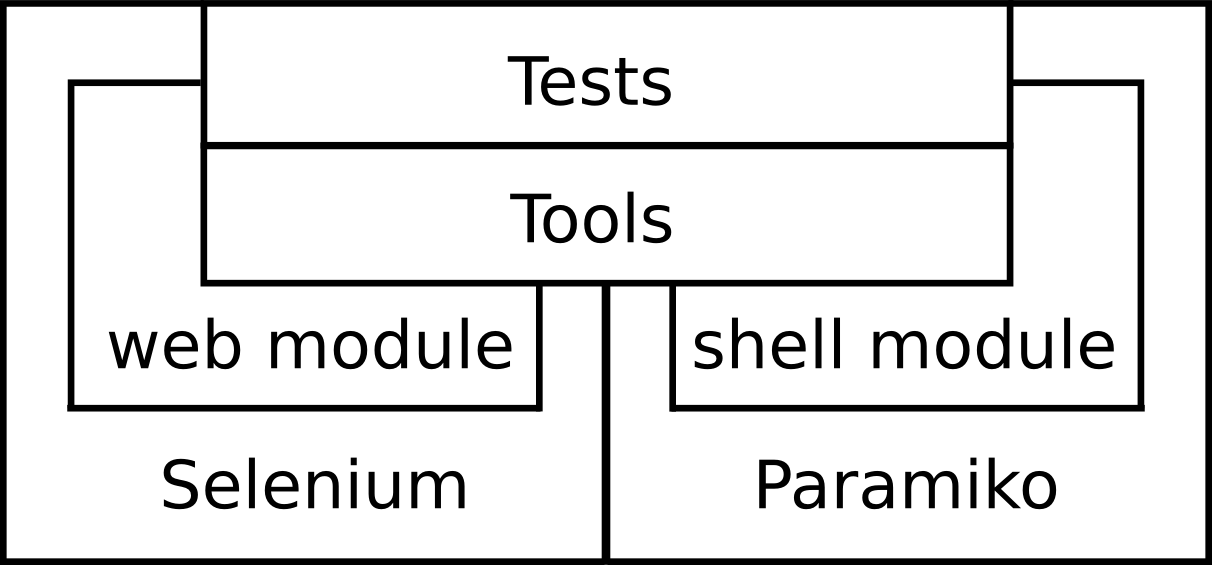
\includegraphics[width=0.5\textwidth]
    {../../images/hubcheck_block_diagram/hubcheck_library_overview_base.png}
  \caption{ The HUBcheck library builds on top of the Selenium and Paramiko libraries. }
  \label{fig:hubzero_library_overview_base}
\end{figure}

The HUBcheck library uses pseudo terminals and web browsers to perform tasks.
Pseudo terminal communication is managed by the \xfmodule{subprocess} and
\xfmodule{paramiko} modules from the Python programming language, while web
browser control is routed through Selenium WebDriver's Python bindings.  The
\xfmodule{hubcheck} package provides web modules and shell modules to perform
many of the redundant tasks required to setup the resources needed to perform
automated tasks.

\section{HUBcheck Web Modules}
\label{sec:hubcheck_web_modules}

\begin{figure}[tbh]
  \centering
  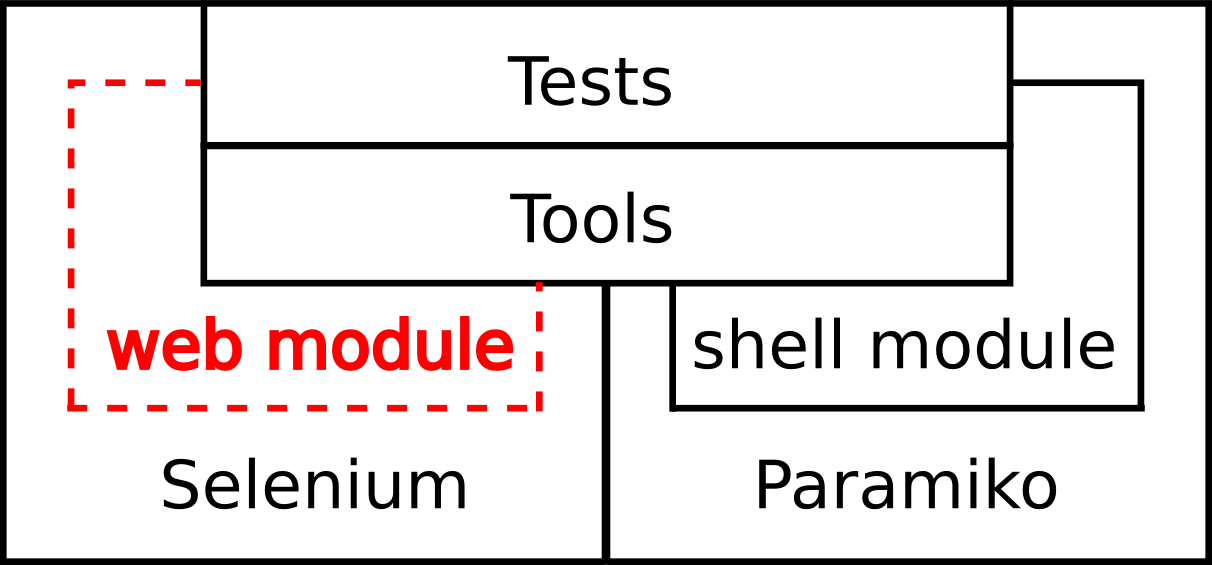
\includegraphics[width=0.5\textwidth]
    {../../images/hubcheck_block_diagram/hubcheck_library_overview_web_module.png}
  \caption{ The HUBcheck library web module can be used to launch browsers and interact with web pages. }
  \label{fig:hubzero_library_overview_web_module}
\end{figure}

HUBcheck relies upon the web browser automation of Selenium WebDriver to manage
tasks being performed on hub websites. Selenium WebDriver provides an abstract
way of controlling a number of different web browsers including Firefox,
Chrome, IE, Safari, and Opera. The most recent releases of HUBcheck support
instantiating a Firefox web browser using the \xfclass{Firefox} class. Once a
web browser has been launched, users can begin to interact with web pages using
HUBcheck's page objects, which provide common functionality for pieces of web
pages.


Consider the use case where an automation script needs to login to the hub
website as a user. In order to complete this task, the script must first launch
a web browser that can be automated. Next the script needs to tell the web
browser to navigate to the hub's login page. Once on the login page, the script
has to fill in the username and password fields, and press the login button.
Finally, the script should check that the login was successful.
\Cref{lst:selenium_ide_hubzero_login} laid out a fragile way to do this with
hard coded web element locators that were embedded inside of the automation
script. This made the script hard to read and difficult to update. An
alternative way to solve the problem, using the HUBcheck library, is shown in
\Cref{lst:hubcheck_hubzero_login}.

\begin{xcode}{%
  language=Python,%
  label=lst:hubcheck_hubzero_login,%
  caption={Login to the hubzero.org website using the HUBcheck library}%
}
import hubcheck

username = 'user1'
password = 'pass1'

hc = hubcheck.Hubcheck(hostname='hubzero.org',
                       locators='hubzero',
                       browsertype='Firefox')

# setup a web browser
hc.browser.get('https://hubzero.org')

# login to the website
po = hc.catalog.load_pageobject('LoginPage')
po.goto_page()
po.login_as(username,password)

# check that the user is logged in
po = hc.catalog.load_pageobject('GenericPage')
assert po.is_logged_in() is True
\end{xcode}

\Cref{lst:hubcheck_hubzero_login} contains no web element locators
directly in the automation script. Instead, it takes advantage of the page
objects that are a part of the HUBcheck library, which makes for a simplified
script that is easy to read and understand.
\Cref{lst:hubcheck_hubzero_login} starts, on line 6, by creating a
\xfclass{Hubcheck} object.  The \xfclass{Hubcheck} object manages both the web
browser and the page objects used in the script. Next, on line 11, the script
uses the \xfclass{Hubcheck} object to launch the web browser and navigate it to
the hub's website. To get to the hub's login page, we load the
\xfclass{LoginPage} page object on line 14 and use its \xfmethod{goto\_page()}
method to handle the navigation. Once on the login page, we employ the page
object's \xfmethod{login\_as()} method to perform the login service of filling in
the username and password fields, and clicking the login button. Lastly, the
script checks that the user was properly logged in by calling the
\xfmethod{is\_logged\_in()} method available in all HUBcheck page objects.

The sections below describe the details of opening a web browser, navigating
the hub, and using the services available through HUBcheck page objects.

\subsection{Configuring HUBcheck}
\label{ssec:hubcheck_web_modules_configure}

HUBcheck supports multiple versions of the HUBzero software, so it is important
that HUBcheck is configured properly before starting the web automation. The
most basic configuration tells HUBcheck the type of web element locators to use
and the URL of the hub where automation will occur. These two pieces of
information can be fed into the \xfclass{Hubcheck} object as parameters during
initialization.

\begin{xcode}{%
  language=Python,%
  label=lst:hubcheck_object_initialization,%
  caption={Configuring a Hubcheck object}%
}
hc = hubcheck.Hubcheck(hostname='hubzero.org',
                       locators='hubzero',
                       browsertype='Firefox')
\end{xcode}

\Cref{lst:hubcheck_object_initialization} demonstrates how to create and
configure a \xfclass{Hubcheck} object. The object allows developers to
configure the hostname of the hub under automation, the page objects that
should be used during automation, and the web browser to automate. The HUBcheck
library has page objects and web element locators from 19 of the hubs managed
by the HUBzero Team, as well as a few of the latest open source
releases. Popular locators to use include \xflocator{hubzero}, for the hubzero.org
website, and \xflocator{osr\_1\_3\_0}, for the open source release available at
the time of writing.

% Not all pages on the hub have page objects available to them.

The \xfclass{Hubcheck} object is a thin layer over three much more powerful
objects, the browser object, the catalog object and the utils object. The next
few sections discuss how these three objects are used while building HUBcheck
based web automation tools.

\subsection{Launching a Browser With the Browser Object}
\label{ssec:hubcheck_web_modules_launch_browser}

HUBcheck provides classes, representing each of the supported web browsers, to
make launching a web browser simple and fast.  The browser classes build upon
Selenium WebDriver browser objects, setting up preferences, loading browser
extensions helpful for debugging, and attaching the browser to a proxy for HTTP
response inspection.  When a \xfclass{Hubcheck} object is created, it includes
a browser object that can be used to launch a web browser by calling the
\xfmethod{get()} method.

\begin{xcode}{%
  language=Python,%
  label=lst:hubcheck_object_launch_browser,%
  caption={Launching a Firefox web browser using the Hubcheck object}%
}
hc.browser.get('https://hubzero.org')
\end{xcode}

The type of browser launched is controlled by the \xfparameter{browsertype}
argument of the \xfclass{Hubcheck} object's initialization. If no browsertype
is set, the object defaults to launching a Firefox web browser.

Behind the scenes, the \xfclass{Hubcheck} object is calling HUBcheck's
\xfclass{Firefox} class. The \xfclass{Firefox} class is responsible for setting
up the browser profile, attaching the browser to a web proxy, and launching the
browser. The same class could be called, directly by the developer, to get a
stand-alone browser object as shown in \Cref{lst:hubcheck_launch_browser}.

\begin{xcode}{%
  language=Python,%
  label=lst:hubcheck_launch_browser,%
  caption={Launching a stand-alone Firefox web browser using HUBcheck's \xfclass{Firefox} class}%
}
browser = hubcheck.browser.Firefox()
browser.get('https://hubzero.org')
\end{xcode}

\subsection{Navigating the Hub With the Catalog Object}
\label{ssec:hubcheck_web_modules_navigation}

The HUBcheck library provides page objects that express the services available
on hub web pages. Automation developers can use these page objects to ease
navigation through the hub website, perform tasks on hub web pages, or to build
new page objects using HUBcheck's widgets.

The HUBcheck library's page objects are contained within Python modules.
Additionally, each hub has a module defining which page objects work with the
hub.  These modules are accessible through the \xfobject{hubcheck} object's
\xfattribute{catalog} attribute, which is an instance of the
\xfclass{PageObjectCatalog} class.  Through the \xfattribute{catalog} attribute's
\xfmethod{load\_pageobject()} method, users instantiate new page objects
appropriate for the hub being automated.

\begin{xcode}{%
  language=Python,%
  label=lst:load_hubcheck_page_object,%
  caption={Loading a HUBcheck page object for hub navigation}%
}
# load the LoginPage page object
po = hc.catalog.load_pageobject('LoginPage')
po.goto_page()
po.login_as('testuser','pass123')
\end{xcode}

\Cref{lst:load_hubcheck_page_object} shows an example of loading the
\xfclass{LoginPage} page object, for the login web page, and assigning it to the
variable \xfparameter{po} in line 2. The script goes on to call the page object's
\xfmethod{goto\_page()} method, which is a general page object service for
navigation, and the \xfmethod{login\_as()} method, which represent a service
available on the login web page. The login web page offers several other
services like navigating to the username remind page, navigating to the
password reset page, navigating to the hub registration page, and submitting a
support ticket. All of these services are available through methods of the
LoginPage page object.


% FIXME: need to talk about the utils class
%        can mention that some of the more common actions have been made available
%        as a single method call to the utils class, like the login_as() method
%        listed above.

\subsection{Performing Common Tasks With the Utils Object}
\label{ssec:hubcheck_web_modules_common_tasks}

Automation scripts often contain repeated bits of code that perform common
tasks like logging into a website or uploading a resource. Many times the code
required to perform these tasks is copied between scripts. For large tasks,
copying code between scripts reduces code maintainability.  The HUBcheck
library provides developers with the \xfobject{utils} object which holds
functions for commonly performed tasks related to user accounts, support
tickets, and tool resource contribution.


\begin{xcode}{%
  language=Python,%
  label=lst:hubcheck_utils_login,%
  caption={Common hub tasks are made easier using the methods from the utils object}%
}
import hubcheck

username = 'user1'
password = 'pass1'

hc = hubcheck.Hubcheck(hostname='hubzero.org',
                       locators='hubzero',
                       browsertype='Firefox')

# setup a web browser
hc.browser.get('https://hubzero.org')

# login to the website
hc.utils.account.login_as(username,password)

# check that the user is logged in
po = hc.catalog.load_pageobject('GenericPage')
assert po.is_logged_in() is True
\end{xcode}

Previously, \Cref{lst:hubcheck_hubzero_login} demonstrated using the
\xfclass{LoginPage} page object and its \xfmethod{login\_as()} method to fill
in and submit the hub login form. Logging into a hub website is such a
frequently performed task, it was included as a part of the \xfclass{utils}
class. In \Cref{lst:hubcheck_utils_login}, the code that used to load
the \xfclass{LoginPage} page object, navigate to the login web page, and fill
in the login form has been replaced with a call to
\xfmethod{hc.utils.account.login\_as()}.


\section{HUBcheck Shell Modules}
\label{sec:hubcheck_shell_modules}

\begin{figure}[tbh]
  \centering
  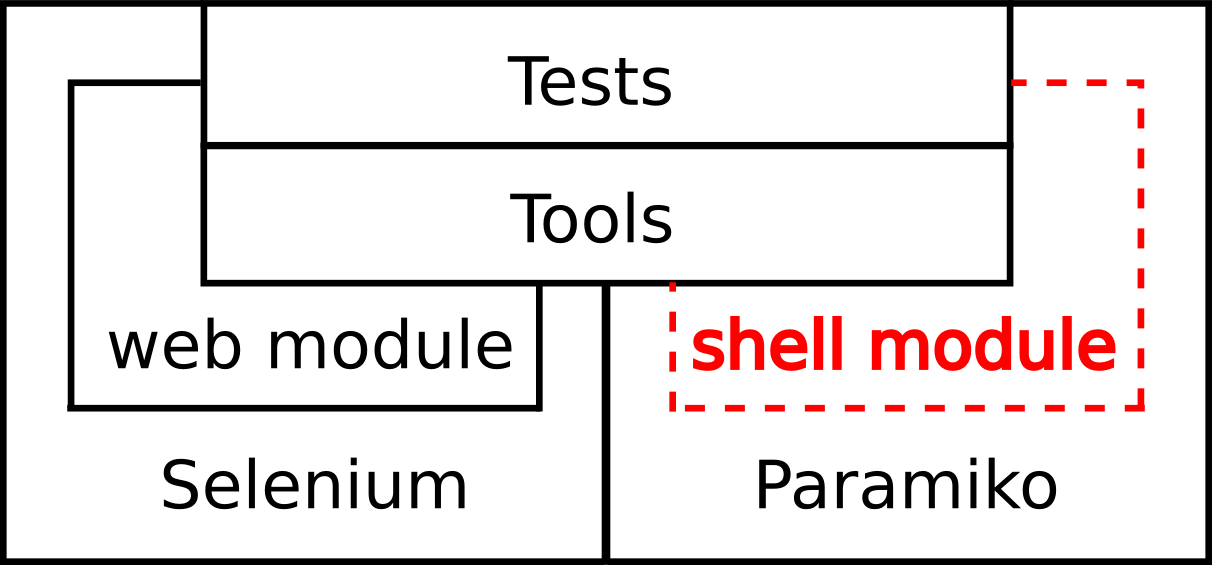
\includegraphics[width=0.5\textwidth]
    {../../images/hubcheck_block_diagram/hubcheck_library_overview_shell_module.png}
  \caption{ The HUBcheck library shell module can be used to SSH into systems and interact through the command line. }
  \label{fig:hubzero_library_overview_shell_module}
\end{figure}

The HUBcheck library also supports automation of shell utilities that run over
Secure SHell Version 2 (SSHv2), the protocol used to create encrypted channels
to services hosted on remote machines. The HUBcheck library allows developers
to quickly open interactive shells and \xfprogramname{sftp} sessions for
accessing remote hosts, including the tool session container on the hub.

% Remote Shell Access
% |-hubcheck.SSHClient
%   |-hubcheck.SSHShell
% |-hubcheck.ContainerManager
%   |-hubcheck.ToolSession
%     |-hubcheck.ToolSessionShell
% Remote File Transfer
% |-hubcheck.SFTPClient
\subsection{Starting a Remote SSH Session}
\label{ssec:starting_remote_ssh_session}

The \xfclass{hubcheck.SSHClient} class can be used to start an SSH session. The
class allows for two ways to login to the remote host, either by providing a
username and password or by providing a username and key filename, where the
key filename is a file, or list of filenames, of private keys for SSH
authentication.


\begin{xcode}{%
  language=Python,%
  label=lst:ssh_client_object,%
  caption={Connecting to a remote host over SSH}%
}
import hubcheck

sh = hubcheck.SSHClient(host='hubzero.org',
                        username='testuser',
                        password='pass123')
\end{xcode}

Upon successful authentication, an \xfclass{SSHShell} object is returned. The
\xfclass{SSHShell} object can be used to interact with the shell in a manner
similar to Expect by using calls to \xfmethod{send()} and \xfmethod{expect()}
methods.  The \xfmethod{send()} method is used to run commands over the remote
channel. It accepts a single parameter, the command to be run. The
\xfmethod{expect()} method is used to retrieve output from the remote channel's
buffer. It accepts a list of patterns and tries to match each pattern to the
data in the channel's buffer.  If it finds a match, the matching data is stored
and the method returns the index of the pattern that matched the data.
\Cref{lst:ssh_shell_send_expect} shows examples of using the \xfmethod{send()}
and \xfmethod{expect()} methods.

\begin{xcode}{%
  language=Python,%
  label=lst:ssh_shell_send_expect,%
  caption={Using the Expect like interface of SSHShell}%
}
sh.send('echo hi')
r = sh.expect('hi')
# r == 0, the index of the matched pattern 'hi'

sh.send('echo hi')
r = sh.expect(['tie','hi','bye',sh.TIMEOUT])
# r == 1, the index of the matched pattern 'hi'

sh.send('echo hi')
r = sh.expect(['cry',sh.TIMEOUT])
# r == -1, no patterns matched, expect() timed out
\end{xcode}

The \xfmethod{expect()} method uses Python's regular expression module,
\xfmodule{re}, and can accept complicated regular expressions as patterns. If
the pattern argument contains a regular expression that is matched to data in
the channel's buffer, the resulting \xfobject{re.match} object is stored in the
SSHShell object's \xfparameter{match} attribute, where the developer can query
it further for the exact text and groupings that were matched.
\Cref{lst:ssh_shell_expect_match} shows how to access matches found by the
\xfmethod{expect()} method.

\begin{xcode}{%
  language=Python,%
  label=lst:ssh_shell_expect_match,%
  caption={Using a regular expression as a pattern in the expect() method}%
}
# grab the prompt and escape it for use in a regular expression
import re
prompt = re.escape(sh.get_prompt())

# match any string
sh.send('echo hi')
sh.expect(['(.*){0}'.format(prompt)])
# the matching text is stored in a re.match object, available through sh.match
result = sh.match.groups()[0]
# result == 'hi\r\n'
\end{xcode}


\subsection{Accessing a Hub's Tool Session Container Using SSH}
\label{ssec:hubcheck_shell_modules_accessing_container_ssh}

Tool session containers on the hub can be accessed via an SSH connection, but
SSH'ing into one can be a little tricky due to the hub configuration. All
connections to the hub are routed through the the hub's web server, including
connections destined for the web server and connections destined for tool
session containers. For example, on the imaginary hub named
\xfhtmllink{myhub.org}, a developer, with elevated permissions to login
directly on the web server, would use the command shown in
\Cref{lst:ssh_hub_webserver} to login to the hub's web server.

\begin{xcode}{%
  language=bash,%
  label=lst:ssh_hub_webserver,%
  caption={SSH'ing into a hub's webserver}%
}
ssh user@myhub.org
\end{xcode}

In order to SSH into a tool session container hosted on the hub, the developer
needs to use the hub's VirtualSSH proxy interface provided by the
\xfprogramname{session} command, as shown in
\Cref{lst:ssh_hub_container}.

\begin{xcode}{%
  language=bash,%
  label=lst:ssh_hub_container,%
  caption={SSH'ing into a hub's tool session container}%
}
ssh -t -X user@myhub.org session
\end{xcode}

Normal users, without the elevated permissions needed to login on the web
server, could use either command to connect to the hub, but in the case of
\Cref{lst:ssh_hub_webserver}, the request would be automatically
forwarded into a tool session container.

HUBcheck provides the \xfclass{ToolSession} class to help developers connect to
tool session containers through the hub's VirtualSSH proxy. The
\xfclass{ToolSession} class offers methods analogous to commands of the
VirtualSSH proxy including the ability to start, stop, access, and list
available tool session containers for a user with a password.
\Cref{tab:virtualSSHToolSession} outlines the equivalent ToolSession methods for
each of the Virtual SSH commands.

\begin{table}
  \centering
  \caption{HUBcheck's ToolSession class gives developers easy access to the
           hub's Virtual SSH Commands.}
  \begin{tabular}{ l | l }
    \hline
    ssh [flags] [user@]hostname [command] & ts = ToolSession( \\
                                          &   host,port,username,password) \\
                                          &                       \\
                                          &                       \\ \hline
    Virtual SSH Commands                  & ToolSession Object Methods \\ \hline
                                          &                       \\
    session create [session\_title]       & create(title=None)    \\
                                          &                       \\
    session start                         & start()               \\
                                          &                       \\
    session [session\_number] [command]   & access(snum=None,command=None) \\
                                          &                       \\
    session list                          & list()                \\
                                          &                       \\
    session stop session\_number          & stop(session\_number) \\
                                          &                       \\
    session help                          & help()                \\
                                          &                       \\
    \hline
  \end{tabular}
  \label{tab:virtualSSHToolSession}
\end{table}


\subsubsection{Starting a Tool Session Container With HUBcheck}
\label{ssec:hubcheck_shell_modules_starting_container}

VirtualSSH provides two ways to start a tool session container, using the
\xfprogramname{session create} or \xfprogramname{session start} subcommands.
The \xfprogramname{session create} subcommand initiates the creation of a tool
session container, allowing the developer to name the container by setting the
\xfparameter{session\_title} parameter.  After calling the
\xfprogramname{session create} subcommand, the user is returned to their local
shell with a session number they can connect to.  Similarly, the
\xfprogramname{session start} subcommand also initiates the creation of a tool
session container, but goes the extra step of placing the user into the
container where they can run shell commands on the remote host.

\begin{xcode}{%
  language=bash,%
  label=lst:virtualssh_start_tool_session_container,%
  caption={Starting a hub tool session container using VirtualSSH}%
}
ssh user@myhub.org session create
# 40023, a session number is returned to the user

ssh user@myhub.org session create mytitle
# 40023, a session number is returned to the user

ssh user@myhub.org session start
# user is placed into the tool session container
\end{xcode}

HUBcheck's \xfclass{ToolSession} class provides access to these subcommands
through the \xfmethod{create()} and \xfmethod{start()} methods. Just like
VirtualSSH's \xfprogramname{session create} subcommand, the \xfmethod{create()}
method accepts an optional session title, but it returns three Paramiko
\xfclass{ChannelFile} objects that can be treated like Python file objects. One
of the \xfclass{ChannelFile} objects, \xfparameter{stdout}, holds the session
number of the newly created session. The \xfclass{ToolSession} class's
\xfmethod{start()} method accepts no arguments and returns a
\xfclass{ToolSessionShell} object, which is derived from the \xfclass{SSHShell}
class introduced in \Cref{ssec:starting_remote_ssh_session}.
\Cref{lst:toolsession_start_tool_session_container} shows how to create and
start tool session containers using HUBcheck's \xfclass{ToolSession} class.

\begin{xcode}{%
  language=python,%
  label=lst:toolsession_start_tool_session_container,%
  caption={Starting a hub tool session container using the ToolSession class}%
}
import hubcheck

ts = hubcheck.ToolSession(hostname,
                          username = username,
                          password = password)

(stdin,stdout,stderr) = ts.create()
# stdout.read() provides the session number

(stdin,stdout,stderr) = ts.create('mytitle')
# stdout.read() provides the session number

shell = ts.start()
# shell is a ToolSessionShell, a type of SSHShell
\end{xcode}


\subsubsection{Accessing a Tool Session Container With HUBcheck}
\label{ssec:hubcheck_shell_modules_accessing_container}

The default behavior of VirtualSSH's \xfprogramname{session} command is to
place the user into a tool session container.  If the developer has multiple
tool session containers running, they can choose which one to enter by
providing the \xfprogramname{session} command with an integer argument
representing the  session number, a unique integer identifier for a tool
session container. The \xfprogramname{session} command also accepts an optional
\xfparameter{command} argument.  When the \xfparameter{command} argument is
provided, \xfprogramname{session} will execute the command in the tool session
container and return the user to the local shell along with the stdout and
stderr streams from the command.
\Cref{lst:virtualssh_access_tool_session_container} shows how VirtualSSH's
\xfprogramname{session} command can be used to get into a tool session
container with no arguments, with a session number, and with a command.

\begin{xcode}{%
  language=bash,%
  label=lst:virtualssh_access_tool_session_container,%
  caption={Accessing a hub tool session container using VirtualSSH}%
}
ssh user@myhub.org session
# user is placed into an open tool session container

ssh user@myhub.org session 40023
# user is placed into tool session container with session number 40023

ssh user@myhub.org session "echo hi"
# the command "echo hi" is run in a tool session container.
# "hi" is returned to stdout, user is returned to local shell

ssh user@myhub.org session 40023 "echo hi"
# the command "echo hi" is run in the tool
# session container with session number 40023
# "hi" is returned to stdout, user is returned to local shell
\end{xcode}

The \xfclass{ToolSession} class provides tool session container access through
the \xfmethod{access()} method. The \xfmethod{access()} method accepts two
parameters, representing the session number and the command to run in the tool
session container, just like VirtualSSH's \xfprogramname{session} command.
Example use of the \xfmethod{access()} method is shown in
\Cref{lst:toolsession_access_tool_session_container}.

\begin{xcode}{%
  language=python,%
  label=lst:toolsession_access_tool_session_container,%
  caption={Accessing a hub tool session container using the ToolSession class}%
}
shell = ts.access()
# places user into a tool session container and returns
# a ToolSessionShell object to control the container.

shell = ts.access(session_number=40023)
# places user into tool session container with
# session number 40023, and returns a ToolSessionShell
# object to control the container.

(stdin,stdout,stderr) = ts.access(command='echo hi')
# runs the command 'echo hi' in a tool session container
# returns stdin, stdout, and stderr to the user.

(stdin,stdout,stderr) = ts.access(40023,'echo hi')
# runs the command 'echo hi' in  tool session container
# with session number 40023. returns stdin, stdout, and
# stderr to the user.
\end{xcode}


\subsubsection{Listing Available Tool Session Containers With HUBcheck}
\label{ssec:hubcheck_shell_modules_listing_containers}

VirtualSSH's \xfprogramname{session list} subcommand can be used to get a list of
available tool session containers for a user. For each open tool session
container, the command returns the session number, session name, and session
title. The session name is the name of the tool that started the session. This
is usually a workspace, but could be any of the installed tools on the hub
since they all run in tool session containers. The \xfprogramname{session list}
subcommand also denotes the default tool session container for SSH connections by
using a * in the output column named \texttt{Default}.
\Cref{lst:virtualssh_list_tool_session_containers} shows example output from
VirtualSSH's \xfprogramname{session list} subcommand.

\begin{xcode}{%
  language=bash,%
  label=lst:virtualssh_list_tool_session_containers,%
  caption={Listing available hub tool session containers using VirtualSSH}%
}
ssh user@myhub.org session list
#   Number  Default Name                 Title
#     8374     *    workspace_r1         Workspace (6:57 pm)
#     8584          workspace_r1         Workspace
# Connection to myhub.org closed.
# user is placed back in their local shell
\end{xcode}

This same information can be retrieved programmatically by using the
\xfmethod{list()} method in the \xfclass{ToolSession} class. Similar to running
a command in a tool session container, the \xfmethod{list()} method returns its
output as a 3-tuple whose elements represent the stdin, stdout, and stderr
channels as Python file-like objects.
\Cref{lst:toolsession_list_tool_session_containers} shows an example of using
the \xfclass{ToolSession} class's \xfmethod{list()} method.

\begin{xcode}{%
  language=python,%
  label=lst:toolsession_list_tool_session_containers,%
  caption={Listing available hub tool session containers using the ToolSession class}%
}
(stdin,stdout,stderr) = ts.list()
# returns the list of open sessions to the stdout variable

stdout.read()
#   Number  Default Name                 Title
#     8374     *    workspace_r1         Workspace (6:57 pm)
#     8584          workspace_r1         Workspace
\end{xcode}

To make accessing the information easier, the \xfclass{ToolSession} class also
provides the \xfmethod{get\_open\_session\_detail()} method, which returns the
same information as an iterable Python dictionary, with row numbers as keys and
row data as values.

\begin{xcode}{%
  language=python,%
  label=lst:toolsession_list_tool_session_containers2,%
  caption={Iterating through tool session container details}%
}
import pprint

details = ts.get_open_session_detail()
# returns a dictionary of open session data

pprint.pprint(details)
#{0: {'default': True,
#     'name': 'workspace_r1',
#     'session_number': '8374',
#     'title': 'Workspace (6:57 pm)'},
# 1: {'default': False,
#     'name': 'workspace_r1',
#     'session_number': '8584',
#     'title': 'Workspace'}}

for row in details.values():
  if row['session_number'] == '8584':
    title = row['title']

print title
# Workspace
\end{xcode}


\subsubsection{Stopping Tool Session Containers With HUBcheck}
\label{ssec:hubcheck_shell_modules_stop_containers}

VirtualSSH allows users to stop a tool session container using the
\xfprogramname{session stop} subcommand. The command accepts an integer argument that
specifies the session number that should be stopped.

\begin{xcode}{%
  language=bash,%
  label=lst:virtualssh_stop_tool_session_container,%
  caption={Stopping a hub tool session container using VirtualSSH}%
}
ssh user@myhub.org session stop 40023
# stopping session 40023
# Connection to myhub.org closed.
# user is placed back in their local shell
\end{xcode}

To stop tool session containers using the \xfclass{ToolSession} class, use the
\xfmethod{stop()} method. The \xfmethod{stop()} method accepts a single
parameter, an integer session number specifying the tool session container to
stop.

\begin{xcode}{%
  language=python,%
  label=lst:toolsession_stop_tool_session_containers,%
  caption={Stopping a hub tool session containers using the ToolSession class}%
}
(stdin,stdout,stderr) = ts.stop(40023)
\end{xcode}


\subsection{Managing Tool Session Containers}
\label{ssec:hubcheck_shell_modules_managing_containers}

When writing automated scripts and tests, keeping track of all of the tool
session containers being opened and closed can be a hassle. HUBcheck tries
address this by offering the \xfclass{ContainerManager} class, which promotes
the efficient reuse of tool session containers when possible. The
ContainerManager class is a singleton that can be used to create, access, and
stop tool session containers for multiple users.

Consider the case where several test cases need access to a tool session
container to perform a test. The simple solution would be to have each test
case start, access, and stop a new tool session container to perform its test.
This approach provides isolation between each test, helping ensure
another resource doesn't accidentally close the tool session container while a
test case is using it. It is, however, terribly inefficient. Starting up a tool session
container takes a few seconds and using it for a single, non-destructive
test would be wasteful. Often, an execution of HUBcheck runs hundreds of tests,
the majority of which only query resources in the tool session container,
leaving it in good condition for further use. The approach taken by many
HUBcheck based tools is to reuse tool session containers whenever possible.

The \xfclass{ContainerManager} class helps implement a tool session container
reuse approach. Accessing tool session containers is similar to using the
\xfclass{ToolSession} class directly, but removes most of the rarely used
features. The \xfclass{ContainerManager} class provides an \xfmethod{access()}
method developers can use to enter a tool session container. The
\xfmethod{access()} method takes three parameters, the hostname of the hub
hosting the tool session container, the username and the password of the user
opening the tool session container.  Given this information, the
\xfclass{ContainerManager} class looks in its internal dictionary to see if it
already has a tool session container open for the hostname and username
combination. If it does, a new shell for that container is opened and returned
to the user as a \xfclass{ToolSessionShell} object. If not, a new tool session
container is created and a \xfclass{ToolSessionShell} object is returned.

\begin{xcode}{%
  language=python,%
  label=lst:containermanager_access_tool_session_containers,%
  caption={Accessing a tool session container using the ContainerManager class}%
}
import hubcheck

cm = hubcheck.ContainerManager()

ws1 = cm.access(hostname,username,password)
# ws1 is a ToolSessionShell object

session_number1 = ws1.execute('echo $SESSION')
# '40023'
\end{xcode}

The \xfclass{ContainerManager} can track multiple open tool session containers,
by multiple users, on multiple hubs.  Calling the \xfmethod{access()} method a
second, or a third, time with the same hostname and username results in
additional shells being opened in the same tool session container.

\begin{xcode}{%
  language=python,%
  label=lst:containermanager_multiple_access_tool_session_containers,%
  caption={Multiple accesses to a tool session container using the ContainerManager class}%
}
ws2 = cm.access(hostname,username,password)
# ws2 is another ToolSessionShell object

session_number2 = ws2.execute('echo $SESSION')
# '40023'
\end{xcode}

Calling the \xfmethod{access()} method with a different hostname or username
results in a new tool session container being created.

\begin{xcode}{%
  language=python,%
  label=lst:containermanager_multiuser,%
  caption={ContainerManager can handle multiple users' tool session containers}%
}
ws3 = cm.access(hostname,username2,password2)
# ws3 is another ToolSessionShell object

session_number3 = ws3.execute('echo $SESSION')
# '40024'
\end{xcode}


In many HUBcheck based tools, there is little advantage to closing a tool
session container before the program ends, but for the times when this is
needed, the \xfclass{ContainerManager} class provides the \xfmethod{stop()} and
\xfmethod{stop\_all()} methods. The \xfmethod{stop()} method uses its
parameters, a hostname, username, and session number, to determine which tool
session container to stop.  The \xfmethod{stop\_all()} method loops through all
tool session containers managed by the \xfclass{ContainerMananger} object and
stops them.

\begin{xcode}{%
  language=python,%
  label=lst:containermanager_stop_tool_session_containers,%
  caption={Stopping a tool session container using the ContainerManager class}%
}
cm.stop(hostname,username,session_number)
# stop username's tool session container on host hostname
# with session number session_number

cm.stop_all()
# stop all tool session containers managed by the cm object.
\end{xcode}


\subsection{Interacting With the Tool Session Container}
\label{ssec:hubcheck_shell_modules_interacting_containers}

A \xfclass{ToolSessionShell} object is returned for many of the methods that
access a tool session container. The \xfclass{ToolSessionShell} class is
derived from the \xfclass{SSHShell} class and provides the \xfmethod{send()}
and \xfmethod{expect()} methods described in
\Cref{ssec:starting_remote_ssh_session}. It also provides the
\xfclass{SSHShell}'s \xfmethod{execute()} method, which combines both the
\xfmethod{send()} and \xfmethod{expect()} methods into one function call that
checks the exit status of the executed command. If a command returns a
non-zero exit status, an \xfclass{ExitCodeError} exception is raised, and
command execution stops. In this respect, the \xfmethod{execute()} method acts
like a shell with the \textbf{-e} flag set, where a script will exit
immediately upon error. A successful call to the \xfmethod{execute()} method
returns the output of the command and the exit status of executing the command.

\begin{xcode}{%
  language=python,%
  label=lst:toolsessionshell_execute_method,%
  caption={Interacting with the tool session container using the ToolSessionShell class}%
}
import hubcheck

cm = hubcheck.ContainerManager()

ws = cm.access(hostname,username,password)
# ws is a ToolSessionShell object

out,es = ws.execute('echo hi')

print out
# 'hi'
\end{xcode}

The \xfclass{ToolSessionShell} class provides features specific to working in the shell
of a tool session container. It provides the \xfmethod{importfile()} method to
transfer files from the user's desktop into the tool session container, the
\xfmethod{exportfile()} method to transfer files from the tool session container
to the user's desktop, and a few functions to simplify parsing tool session
container resource files.


\subsection{Transferring Files Between The User Desktop and the Hub}
\label{ssec:hubcheck_shell_modules_sftp}

The hub supports three methods of transporting files between the user desktop
and the user's hub account, including \xfurischeme{webDAV},
\xfurischeme{filexfer}, and \xfurischeme{sftp}. HUBcheck provides ways to use
\xfurischeme{filexfer} and \xfurischeme{sftp}, while the Python module
\xfmodule{webdavlib} \cite{WebDAVLib:Online} provides a reliable client-side
interface for the \xfurischeme{webDAV} \cite{WebDAV:Online} protocol.

% FIXME: \cite webdavlib
% https://launchpad.net/python-webdav-lib

% FIXME \cite webdav protocol
% https://tools.ietf.org/html/rfc4918
% https://en.wikipedia.org/wiki/WebDAV

The hub's \xfurischeme{filexfer} protocol consists of two commands,
\xfprogramname{importfile} and \xfprogramname{exportfile}. Filexfer transfers
start on the command line of a tool session container's X terminal, by issuing
the the \xfprogramname{importfile} command to transfer files from the user's
desktop into their hub account, or the \xfprogramname{exportfile} command
to transfer files from the user's hub account into their desktop. The
\xfurischeme{filexfer} commands use the tool session container's
\xfprogramname{clientaction} program to initiate a popup window in the user's
web browser. When importing a file, the user populates the popup window with
the text or filename they would like transferred into their hub account. After
submitting the form in the popup window, the data is then saved in the hub
account. When exporting a file, the popup window contains the data of the file
from the user's hub account.

To implement simple file transfers, the \xfclass{ToolSessionShell} class
provides the \xfmethod{importfile()} and \xfmethod{exportfile()} methods. Both
methods take two arguments representing a local filename from inside of the
workspace and a remote filename from the user's desktop. The direction of
transfer is determined by the method being called. Under the hood, these two
functions approximate the actions being performed by the hub's
\xfurischeme{filexfer} commands, by using the \xfurischeme{sftp} protocol to
transfer the files. It is possible to use HUBcheck's web module in coordination
with the \xfclass{ToolSessionShell} class to more closely imitate what users
would really do on the hub, but the goal of the implementation is to transfer
files and, on the command line, using \xfurischeme{sftp} is more efficient.

\begin{xcode}{%
  language=python,%
  label=lst:toolsessionshell_filexfer,%
  caption={Transferring files using ToolSessionShell's importfile and exportfile methods}%
}
import hubcheck

cm = hubcheck.ContainerManager()

ws = cm.access(hostname,username,password)
# ws is a ToolSessionShell object

# importing a file from the desktop to the hub account
ws.importfile('desktop_file.txt', 'hub_file.txt')

# importing data from the desktop to a file in the hub account
file_data = 'transferring is easy'
fsize = ws.importfile(file_data, 'hub_file.txt', is_data=True)
assert fsize == len(file_data)

# exporting a file from the hub account to the desktop
ws.exportfile('hub_file.txt', 'desktop_file.txt')

\end{xcode}

For more control over how files are transferred, the HUBcheck library also
provides access to Paramiko's \xfclass{SFTPClient} class.  HUBcheck's
\xfclass{SFTPClient} class is a small wrapper class around the Paramiko
\xfclass{SFTPClient} class, which can be used to access a user's hub account
through the \xfurischeme{sftp} protocol. With this method, users have full access
to \xfurischeme{sftp} functions like \xfmethod{get}, \xfmethod{put},
\xfmethod{remove}, \xfmethod{chmod}, \xfmethod{open}, \xfmethod{chdir}, and
more.

\begin{xcode}{%
  language=python,%
  label=lst:sftpclient,%
  caption={Transferring files using the SFTPClient class}%
}
import hubcheck

sftp = hubcheck.SFTPClient(hostname,username=username,password=password)
# sftp is a Paramiko SFTPClient object

# transfer file from the hub account to the desktop
sftp.get('hub_file.txt','desktop_file.txt')

# transfer file from the desktop to the hub account
sftp.put('desktop_file.txt','hub_file.txt')

# close the sftp connection
sftp.close()
\end{xcode}

% HUBcheck Tools
% |-tool.py
%   |-parsing command line options and config files
%     |-focus on hubcheck features:
%       hubcheck configuration file
%       logfile/loglevel
%       usage, showing, recording of virtual display
%       highlight web elements as they are searched for
%       scrolling web page to view web elements being interacted with
%       directories for screenshots and videos
%       port for running web proxy
%       smtp setting for emailing results
%   |-setup logging
%   |-xvfb setup (with window manager, and recording, and viewing)
%     |-pyvirtualdisplay is used to start the virtual display
%     |-icewm window manager also started
%     |-hub
%   |-web proxy configuration
%     |-browsermob proxy is used as the web proxy
%     |-use the port from the command line or config file option
%   |-running the command
% |-building your own tool
%   |-subclass hubcheck.Tool
%   |-adding command line or config file options
%   |-define a command() method
%   |-make your module a standalone program
% |-examples
%   |-test runner (hctestrunner)
%   |-nightly rappture builds
%     |-hcnrb.py (trunk and branch-1.3)
%     |-hcnrb_tests_lang_tcl.py
%   |-test user tools
%     |-profile update (hcuserprofile)
%     |-account registration (register_account)
%     |-password change (hcpwc)
%   |-solarpv database update (solarpv_db_update.py)

\section{Building Applications Backed by the HUBcheck Library}
\label{sec:building_hubcheck_backed_applications}

\begin{figure}[tbh]
  \centering
  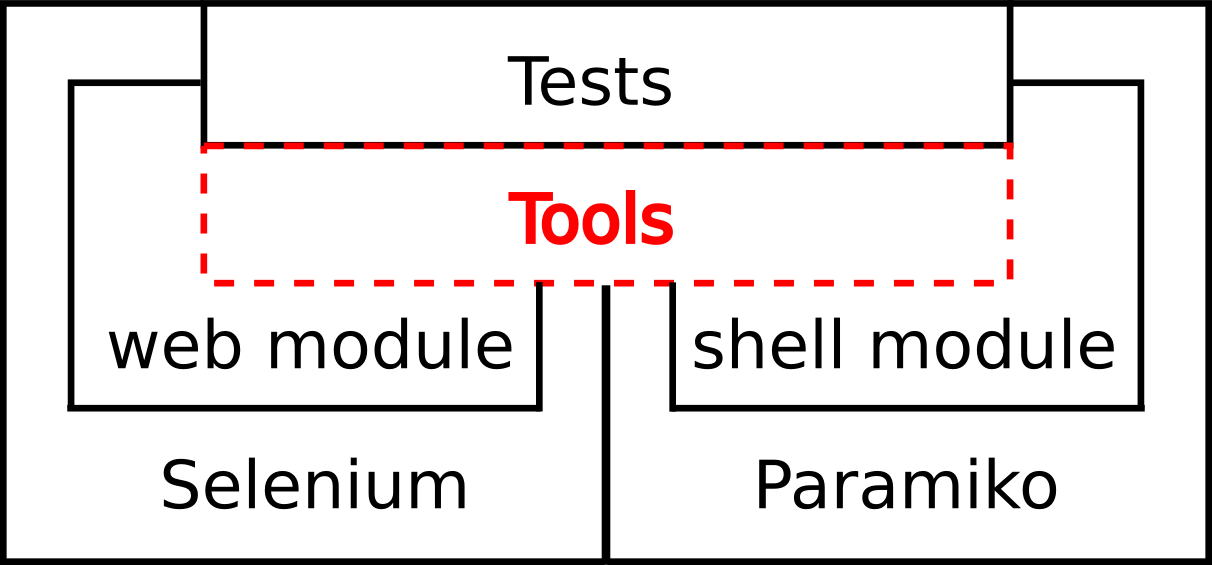
\includegraphics[width=0.5\textwidth]
    {../../images/hubcheck_block_diagram/hubcheck_library_overview_tools.png}
  \caption{ Command line utilities can be built on top of the HUBcheck %
            library by using the \xfclass{hubcheck.Tool} class. }
  \label{fig:hubzero_library_overview_tools}
\end{figure}

The HUBcheck library includes several programs that build upon the web and
shell modules. While each program has a different goal, there are features
common to all of them, like configuration options and environment setup, that
are tedious to write for one program and inefficient to copy for multiple
programs. For this reason, HUBcheck includes the \xfclass{hubcheck.Tool} class,
which can be subclassed to get a common set of command line and configuration
file options with an intuitive parser, automatic logging setup, a virtual
display for running web browser based automation, and a web proxy to help
monitor, block and analyze communications between a web browser and a web site.

Below, we explore the features of \xfclass{hubcheck.Tool} based programs by
building an example tool that performs a user login through the hub's web
and SSH interfaces.

\subsection{Building a Tool}
\label{ssec:building_a_tool}

\xfclass{hubcheck.Tool} is a base class for command line tools that use the
HUBcheck library. The class provides many of the boilerplate features that are
repeated in HUBcheck based programs. By subclassing \xfclass{hubcheck.Tool},
users can quickly create a feature rich command line tool for automating web
and shell access on the hub.

\begin{xcode}{%
  language=python,%
  label=lst:hc_tool_template,%
  caption={HUBcheck based tools follow this general template}%
}
import hubcheck

class LoginTool(hubcheck.Tool):
    def __init__(self,logfile='hcutils.log',loglevel='INFO'):
        super(LoginTool,self).__init__(logfile,loglevel)
        # introduce new command line and configuration options

        # parse command line / config file options, start logging
        self.parse_options()
        self.start_logging()

    def command(self):
        # add code that does the work

if __name__=='__main__':
    tool = LoginTool()
    tool.run()
\end{xcode}


There are three steps to creating a new HUBcheck based tool:

\begin{enumerate}
\item Subclass \xfclass{hubcheck.Tool} to create a new tool class.
\item Populate the tool's \xfmethod{\_\_init\_\_()} and \xfmethod{command()} methods.
\item Call the \xfmethod{run()} method of an instance of the tool's class.
\end{enumerate}

\noindent \Cref{lst:hc_tool_template} shows the general template for HUBcheck
based tools.  The template starts by subclassing \xfclass{hubcheck.Tool} into a
class named \xfclass{LoginTool}, the name of the tool we are creating.
\xfclass{hubcheck.Tool}'s \xfmethod{\_\_init\_\_()} method takes care of
setting up command line and configuration file option parsing, so it is
important that it is called early in the object creation process. In
\Cref{lst:hc_tool_template}, this happens in line 5. \xfclass{hubcheck.Tool}'s
\xfmethod{\_\_init\_\_()} method sets up five variables that can be used by the
\xfclass{LoginTool} class:

\begin{enumerate}
\item \xfparameter{self.command\_parser}
\item \xfparameter{self.config\_parser}
\item \xfparameter{self.options}
\item \xfparameter{self.logger}
\item \xfparameter{self.testdata}
\end{enumerate}

\noindent
The first two, \xfparameter{self.command\_parser} and \xfparameter{self.config\_parser},
are parsers for options set on the command line or in an INI-style
configuration file. You can manipulate these variables inside of
\xfmethod{\_\_init\_\_()}, using their \xfmethod{add\_argument()} and
\xfmethod{add\_option()} methods respectively, to add new options that the
parsers will recognize.

\begin{xcode}{%
  language=python,%
  label=lst:hc_tool_template_add_command_line_flag,%
  caption={Use the \xfmethod{add\_argument()} method to define new command line flags for the tool}%
}
    def __init__(self,logfile='hcutils.log',loglevel='INFO'):
        ...
        # introduce new command line and configuration options
        self.command_parser.add_argument(
            '--video-filename',
            help='name of the video file',
            action="store",
            dest="videofn",
            default='password_change.mp4',
            type=str)
        ...
\end{xcode}

The \xfclass{hubcheck.Tool} class includes functionality to record the virtual
display where the web browser window is running, but does not expose the
ability to name the file that the recording is saved to. Adding a
\xfparameter{-\--video-filename} flag to a tool allows the user to specify the
name of the file where video recordings should be saved.
\Cref{lst:hc_tool_template_add_command_line_flag} shows an example of adding
the new \xfparameter{-\--video-filename} flag to the command line parser.
With the new flag in place, the program can be invoked as shown in
\Cref{lst:hc_tool_username_invoke}.


\begin{xcode}{%
  language=bash,%
  label=lst:hc_tool_username_invoke,%
  caption={Invoking a HUBcheck based tool with a new command line option}%
}
./logintool --config hub.conf --video-filename myvideo.mp4 testuser2
\end{xcode}



%The hubcheck.Tool class provides a command line argument parser,
%self.command\_parser, and an INI style configuration file parser,
%self.config\_parser. Both parsers are configurable from within
%CheckPasswordTool's \_\_init\_\_ method. \textit{hubcheck.Tool} allows users
%to record a mp4 video of the web browser and sometimes it is convenient to
%allow the user to also specify the name of the file the video is recorded to.
%This extra command line parameter can be added inside CheckPasswordTool's
%\_\_init\_\_ method, by using the command parser's \textit{add\_argument}
%method. \Cref{fig:hc_tool_template_add_command_line_flag} demonstrates how to
%do this with the \textit{--video-filename} command line flags.


The \xfmethod{self.parse\_options()} method is called to perform the command
line and configuration file option parsing.  It resolves conflicts and stores
the collected options in the variable named \xfparameter{self.options}.  In
\Cref{lst:hc_tool_template_add_command_line_flag}, line 8 defines the value
obtained from the \xfparameter{-\--video-filename} command line argument to be
stored in the variable \xfparameter{self.options.videofn}.  Before exiting
initialization, \xfmethod{\_\_init\_\_()} starts a logger,
another benefit of subclassing the hubcheck.Tool class. From within the tool,
the logger is accessible through the \xfparameter{self.logger} variable.

The \xfmethod{command()} method is responsible for performing the main tasks of
the program. The method is called indirectly when the object's \xfmethod{run()}
method is executed. In the template shown in \Cref{lst:hc_tool_template}, this
is done at the end of the script on line 17.  The run() method takes care of
much of the setup and teardown of the environment from which the automation
takes place.  It is responsible for loading the HUBcheck configuration data,
setting up directories for browser screenshots and videos, starting a virtual
display for the browser to run in, and launching a web proxy for the web
browser. The \xfmethod{run()} method prepares the environment so the tasks in
the \xfmethod{command()} method can launch a browser with minimal additional
system configuration. After setting up the environment, \xfclass{run()} calls
the tool's \xfclass{command()} method.

A HUBcheck tool's \xfmethod{command()} method holds the objectives of the tool.
Generally, the \xfmethod{command()} method starts by evaluating the command
line and configuration file options, setting local variables based on the
parsed options.

\begin{xcode}{%
  language=python,%
  label=lst:hc_tool_command_part_1,%
  caption={The command() method of a HUBcheck based tool}%
}
    def command(self):
        # set variables based on parsed options
        username = self.options.remainder[0]
        videofn = self.options.videofn

        # retrieve account information
        userpass = self.testdata.find_account_password(username)

        # grab hub configuration from the testdata file
        locators    = self.testdata.get_locators()
        hostname    = self.testdata.find_url_for('https')
        url = "https://%s" % (hostname)

        # create a hubcheck object
        hc = hubcheck.Hubcheck(hostname=hostname,locators=locators)

        # initialize recording
        self.start_recording_xvfb(videofn)
        ...
\end{xcode}

In the \xfmethod{command()} method for our example \xfprogramname{logintool}
program, shown in \Cref{lst:hc_tool_command_part_1}, lines 9 - 11 introduce the
use of the \xfparameter{self.testdata} variable, which is setup by the
\xfclass{hubcheck.Tool} class.  \xfparameter{self.testdata} is an instance of
HUBcheck's \xfclass{TestData} class, which provides helper methods for querying
information from a HUBcheck configuration file.  \xfparameter{self.testdata}
gives developers access to information about which HUBcheck web element
locators, test user account information, and hub URLs to use. With hub specific
information acquired, the program creates a HUBcheck browser object in line 15
and starts recording the virtual display in line 18.

The next step is to login to the hub through the web interface.
\Cref{lst:hc_tool_command_part_2} uses the \xfobject{hc} object's
\xfparameter{browser} and \xfparameter{utils} attributes to open a web browser,
login to the web site, logout of the web site, and close the browser.

\begin{xcode}{%
  language=python,%
  label=lst:hc_tool_command_part_2,%
  caption={Login through the web interface}%
}
    def command(self):
        ...
        # start up a selenium webdriver based browser
        hc.browser.get(url)

        # login to the hub using the web interface
        hc.utils.account.login_as(username,userpass)

        # navigate to the dashboard and logout
        hc.utils.account.logout()

        # close the browser and cleanup
        hc.browser.close()
        self.stop_recording_xvfb()
        ...
\end{xcode}

\noindent
Similarly, \Cref{lst:hc_tool_command_part_3} uses a \xfclass{ToolSession}
object to login to a tool session container through the SSH interface.

\begin{xcode}{%
  language=python,%
  label=lst:hc_tool_command_part_3,%
  caption={Login through the Virtual SSH interface}%
}
    def command(self):
        ...
        # login to the hub using the Virtual SSH interface
        ts = hubcheck.ToolSession(
              hc.hostname, username=username, password=userpass)

        # SSH into a tool container and run the 'echo hi' command
        stdin,stdout,stderr = ts.access(command='echo hi')

        # check stdout for the output of the command, 'hi'
        output = stdout.read(1024)
        assert output == 'hi\n', \
            "error ssh'ing into tool container: %s" % (output)
\end{xcode}


After the \xfmethod{command()} method exits, control is returned to the
\xfmethod{run()} method, which stops the web proxy, shuts down the virtual
display, and performs cleanup actions in the environment.


% FIXME: add some kind of subsection conclusion here
%        how to run the tool
%        what environment features are setup
%        what happens on error?


\subsection{Example Tools}
\label{ssec:hubcheck_tools_examples}

%   |-test runner (hctestrunner)
%   |-nightly rappture builds
%     |-hcnrb.py (trunk and branch-1.3)
%     |-hcnrb_tests_lang_tcl.py
%   |-test user tools
%     |-profile update (hcuserprofile)
%     |-account registration (register_account)
%     |-password change (hcpwc)
%   |-solarpv database update (solarpv_db_update.py)

The \xfmethod{command()} method for the \xfprogramname{logintool} program is
pretty elementary, but any task can be substituted in. Nearly all of the tools
in the HUBcheck library use this subclassing and \xfmethod{command()} method
design pattern as a foundation for the tool's operation. Listed below are a few
tools built upon the HUBcheck library.

\subsubsection{Nightly Rappture Builds}
\label{sssec:hubcheck_tools_examples_hcnrb}

The Rappture Toolkit \cite{RapptureToolkit:Online} is a library that helps
people build and deploy simulation tools with graphical user interfaces. The
library includes a set of Tcl/Tk based graphical user interface widgets and
language bindings for communicating with the GUI in C/C++, Fortran, Ruby,
Matlab/Octave, Java, Perl, and Python.  One part of Rappture testing includes
building and exercising the library inside of a hub tool session container. To
perform these actions, the HUBcheck library is used to get into a hub's tool
session container, build the Rappture Toolkit, and run a number of test suites
on the build. This is the job of the HUBcheck Nightly Rappture Build script,
\xfprogramname{hcnrb}. Once completed, the nightly builds are transferred to
the \xfhtmllink{rappture.org} website where users can download precompiled or
source versions of the library on a nightly basis.

% FIXME:
% cite rappture toolkit
% https://nanohub.org/infrastructure/rappture/wiki/Citations


% FIXME:
% need an image of high level overview of how hcnrb works.
% command line on the left, hcnrb parses options, logs into nanohub container,
% compiles code, runs tests, transfers tars back to download folder, nightly
% cron copies tars to web site.


\subsubsection{Test User Tools}
\label{sssec:hubcheck_tools_examples_tut}

HUBcheck relies on a number of test user accounts setup with different
configurations. Currently, these test accounts are managed in the same way
regular user accounts are managed, through the hub's website interface. To
help manage these accounts' properties, a number of HUBcheck based programs
have been written including an account registration tool, password updating
tool, and a profile management tool.

% FIXME: add an image of the account registration web form.

\xfprogramname{register\_account} is a program built to fill out the account
registration web page. It is generally used shortly after a new hub
installation, to register HUBcheck's test user accounts. Account registration
is a two step process and the \xfprogramname{register\_account} program can be
applied to the first step, filling out the new account registration form. Most
hub registration forms incorporate a CAPTCHA to keep robots from registering
accounts. \xfprogramname{register\_account} does not attempt to interpret the
CAPTCHA. Instead, it leaves time for a human to solve the CAPTCHA. After
filling out the new account registration form, the hub sends a confirmation
email to the user, and the user responds by clicking the link in the email.
This feature is not available in the current version of the
\xfprogramname{register\_account} program, but could show up in a future
version. The \xfprogramname{register\_account} script uses the HUBcheck
library's page objects to manage web page navigation and to populate the
account registration web form.

% FIXME: add an image of the account password change web form.

After test accounts have been created, the focus shifts to maintaining the
accounts. Account maintenance is important in helping reduce the number of
false positives when running tests and to ensure programs can gain the access
they need to accomplish their automated tasks. One of the essential tasks for
managing test accounts is to keep them secure, which includes frequently
changing their passwords. The hub provides a web form for users to change their
passwords and HUBcheck has a page object to automate its use. The
\xfprogramname{hcpwc} program uses the HUBcheck library's page objects to help
automate the generation and updating of test account passwords on the hub.

% FIXME: add an image of the user profile web forms.

Managing the user profile is an account maintenance task that needs to be
performed at least once in the life of the account. The hub user profile holds
information that is usually collected for the purposes of identifying types of
users to the hub's funding agencies, e.g. the National Science Foundation.
Sometimes this information is collected during the account registration
process. Including the information on the new account registration form could
deter people from signing up. As a result the information could be requested
later, when a user wants to use what may be considered a premium service on the
hub. When testing hub components, having account profile update requests popup
unpredictably on a web page may contribute to having false positives in test
results. A solution to this problem is to fully populate the user profile for
all test accounts just after registering the accounts. This is what the
\xfprogramname{hcuserprofile} program does. The components of the hub user profile are
a configurable, yet finite set. \xfprogramname{hcuserprofile} uses HUBcheck's page
objects to navigate to the user profile web page and query the page for a hard
coded list of components that are typically included in hub user profiles. When
a component is found, \xfprogramname{hcuserprofile} attempts to provide a reasonable
response for the component.


\subsubsection{Test Runner}
\label{sssec:hubcheck_tools_examples_hctestrunner}

One of the original motivations for writing HUBcheck was to test the hub. While
HUBcheck has become more than just testing, the test runner is still one of the
most heavily used tools in the library. HUBcheck's test runner tool,
\xfprogramname{hctestrunner}, is a wrapper around \xfprogramname{pytest}, a mature
full-featured Python testing library. \xfprogramname{hctestrunner} uses the
\xfclass{hubcheck.Tool} class to manage the environment in which test cases are
run. The program can be executed from the command line and requires a HUBcheck
configuration file to work.


\begin{xcode}{%
  language=bash,%
  label=lst:hctestrunner_example_execution,%
  caption={hctestrunner accepts hubcheck.Tool flags and pytest flags}%
}
hctestrunner --config ./hubzero.conf -m nightly --collect-only
\end{xcode}

The \xfprogramname{hctestrunner} program accepts the normal set of command line
flags inherited from the \xfclass{hubcheck.Tool} class, and also accepts
command line flags for \xfprogramname{pytest}.
\Cref{lst:hctestrunner_example_execution} shows how to retrieve a list of tests
that are marked with the tag ``nightly'' and would run on
\xfhtmllink{hubzero.org}. To accomplish this, we provide the hubzero.conf
configuration file through \xfclass{hubcheck.Tool}'s \xfparameter{-\--config}
flag, specify the nightly mark through \xfprogramname{pytest}'s
\xfparameter{-m} flag, and ask \xfprogramname{pytest} to only collect tests
(not run them) with the \xfparameter{-\--collect-only} flag.
\xfprogramname{hctestrunner} parses all of the flags, but passes any flags it
does not recognize on to \xfprogramname{pytest}.  After setting up the web
proxy, virtual display and evaluating command line and configuration options,
\xfprogramname{hctestrunner} calls on \xfprogramname{pytest} to manage
searching for and running test cases.

% FIXME:
% need an image to show what is going on in hctestrunner from a high level
% show horizontal picture with hctestrunner command on the left. next box shows
% hctestrunner, next box shows pytest with multiple arrows pointing to the
% right pointing to test cases, some with small web browsers, some with small
% terminals. the test case boxes can point back to the hubcheck library.


% \subsubsection{nanoHUB-U Course Registration Confirmation}

% \subsubsection{SolarPV Database Update}

% FIXME: add an image of how solarpv tool works.




\section{Writing Tests Using the HUBcheck Library}
\label{sec:hubcheck_tests}

\begin{figure}[tbh]
  \centering
  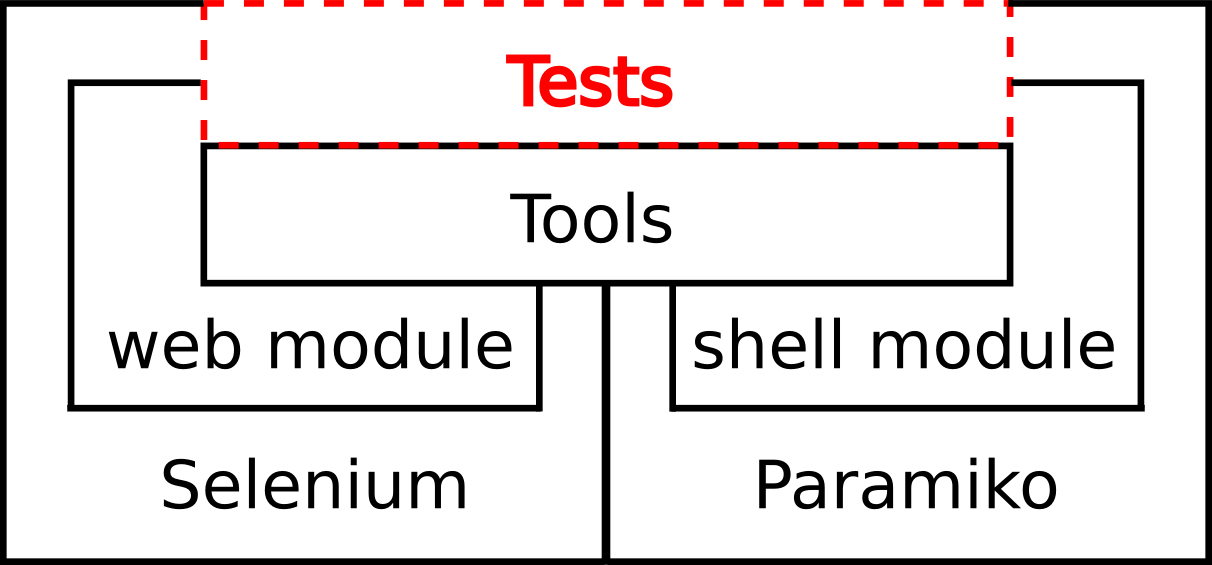
\includegraphics[width=0.5\textwidth]
    {../../images/hubcheck_block_diagram/hubcheck_library_overview_tests.png}
  \caption{ One of HUBcheck's most used features is its test runner and its %
            ability to be embedded within tests. }
  \label{fig:hubzero_library_overview_tests}
\end{figure}

HUBcheck provides the \xfprogramname{hctestrunner} tool to manage the
collection and execution of test cases.  Under the hood,
\xfprogramname{hctestrunner} depends on \xfprogramname{pytest}, a flexible
Python based test case management library that can handle test cases written in
a number of formats including \xfmodule{unittest} \cite{unittest:2015:Online},
\xfmodule{nose} \cite{nose:2015:Online}, and \xfmodule{doctest}
\cite{doctest:2015:Online}.  Section
\ref{sec:building_hubcheck_backed_applications} explored writing programs using
the HUBcheck library, and while test cases can also be written in the same way,
this approach can lead to an excess of code and resource repetition between
test cases. In the following sections, we describe ways to write robust, easy
to understand test cases using the HUBcheck library.

\subsection{Test Fixtures}
\label{ssec:hubcheck_tests_fixtures}

One of the strengths of the \xfprogramname{pytest} library is its flexibility.  Many
test case management libraries include a feature often referred to as a
\textit{test fixture} \cite{TestFixture:Online}.  Test fixtures are functions,
or bits of code, that place the software under test in a fixed state as a
baseline for running tests.

% show example test case noting what would be considered setup and teardown.

Traditionally, x-unit \cite{Xunit:Online} based testing libraries have provided
two types of fixtures: setup fixtures run before a test case, and teardown
fixtures run after the test case. \xfprogramname{pytest} provides a number of
different fixture options which can call upon each other or be reused within
the class, module, or project scopes.

% show example test case using multiple pytest fixtures use different colored
% ablocks to show how fixtures are called before and after a test case

\subsection{The TestCase2 Class}
\label{ssec:hubcheck_tests_testcase2}

HUBcheck provides the \xfclass{TestCase2} class whose purpose is similar to that
of the \xfclass{Tool} class mentioned in Section \ref{ssec:building_a_tool}.
The \xfclass{TestCase2} class provides much of the environment setup and
teardown code needed to run a test and document its behavior in a more detailed
manner than just pass or fail.  The \xfclass{TestCase2} class is responsible for
setting up the filename for browser screenshots, recording individual test
cases to separate video files, setting up test case testdata in local
variables, and managing the page object catalog.  The class also initializes a
local web browser object for each test case.  The \xfclass{TestCase2} class
provides each test case with the following local variables:

\begin{enumerate}
\item \xfparameter{self.browser}
\item \xfparameter{self.catalog}
\item \xfparameter{self.utils}
\item \xfparameter{self.testdata}
\item \xfparameter{self.locators}
\item \xfparameter{self.https\_uri}
\item \xfparameter{self.https\_authority}
\item \xfparameter{self.http\_authority}
\end{enumerate}

\xfclass{TestCase2} hooks into \xfmodule{pytest}'s \xfmethod{setup\_method()} and
\xfmethod{teardown\_method()} test fixtures to provide features similar to that
of HUBcheck based tools.

\subsection{Building a Test Case}
\label{ssec:hubcheck_tests_building}

Consider rewriting the hub website login example, from
\Cref{lst:hubcheck_utils_login}, as a test case.
\Cref{lst:hub_website_login_testcase} demonstrates how to setup a
\xfclass{TestCase2} based test case.  Just like the \xfclass{Tool} class, to use
the \xfclass{TestCase2} class the user first subclasses it.  All classes
derived from \xfclass{TestCase2} have \xfmethod{setup\_method()} and
\xfmethod{teardown\_method()} fixtures, even if it is not explicitly stated in
the derived class as is the case for the \xfmethod{TestHubLogin} class from
\Cref{lst:hub_website_login_testcase}. These two fixtures allow
\xfclass{TestCase2} to perform its variable, browser, page object catalog, and
utility setup before the test case is run, and teardown after the test case has
completed.  In accordance with \xfmodule{pytest}'s test case naming conventions,
all methods of the derived class with names prefixed by \textit{test\_} are
considered test cases.  In \Cref{lst:hub_website_login_testcase}, this
includes the \xfmethod{test\_website\_login()} method.  The test case performs
four tasks.  First, it grabs a username and password from the testdata file in
line 4. Next, it navigates the web browser to the hub's homepage in line 8. In
Line 10, it submits a populated hub login form. Lastly, in line 14, it checks
that the login was successful.


\begin{xcode}{%
  language=python,%
  label=lst:hub_website_login_testcase,%
  caption={Hub website login using HUBcheck's TestCase2 class}%
}
class TestHubLogin(hubcheck.TestCase2):
    def test_website_login(self):
        """ try to login to the hub website """
        self.username,self.userpass = \
            self.testdata.find_account_for('registeredworkspace')

        # setup a web browser
        self.browser.get(self.https_authority)

        self.utils.account.login_as(self.username,self.userpass)

        # verify you have successfully logged in
        po = self.catalog.load_pageobject('GenericPage')
        assert po.header.is_logged_in(),'Login Failed'
\end{xcode}


It is interesting to note how clean and easy to read the
\xfmethod{test\_website\_login()} test case is when compared to the login script
in \Cref{lst:hubcheck_hubzero_login} or even the original login script
in \Cref{lst:selenium_ide_hubzero_login}. Part of the test case's
simplicity is due to its use of the \xfclass{TestCase2} class, which wraps up
most of the standard code needed to setup and teardown the web browser, browser
recording, testdata, page object catalog, and utilities.  Test cases that are
easy to read are often easy to understand and maintain. The \xfclass{TestCase2}
class helps keep test cases short and to the point.

Adding more test cases to the \xfclass{TestHubLogin} class is also easy and
helps demonstrate the power of \xfmodule{pytest}'s fixtures. A complementary
test to logging into the website is logging out. As you might have suspected,
there is a bit of code overlap between the login and logout tests. For example,
in order to test login and logout, both tests need to login.  This common code
can be placed in the \xfmethod{setup\_method()} fixture. In
\Cref{lst:testcase_setup_method}, the code to retrieve the test user
credentials, navigate the browser to the hub's homepage, and login has been
abstracted out of the \xfmethod{test\_website\_login()} test case, and placed
in the \xfclass{TestHubLogin} class's \xfmethod{setup\_method()} fixture. This
fixture and \xfclass{TestCase2}'s \xfmethod{setup\_method()} fixture don't
collide as they would in a normal inheritance situation.  Instead, through the
magic of metaclasses, \xfclass{TestCase2} recognizes the existence of
\xfclass{TestHubLogin}'s \xfmethod{setup\_method()} method, and embeds the
method inside of its \xfmethod{setup\_method()} fixture.  By the time
\xfclass{TestHubLogin}'s \xfmethod{setup\_method()} is called,
\xfclass{TestCase2} has already completed setting up the environment and
variables for the test case. This same embedding happens with
\xfclass{TestHubLogin}'s \xfmethod{teardown\_method()}, but in reverse.
\xfclass{TestCase2} recognizes \xfclass{TestHubLogin}'s
\xfmethod{teardown\_method()} method, calls the method, and then proceeds to
calling its own \xfmethod{teardown\_method()} fixture.

\begin{xcode}{%
  language=python,%
  label=lst:testcase_setup_method,%
  caption={Using pytest fixtures while subclassing the TestCase2 class}%
}
class TestHubLogin(hubcheck.TestCase2):
    def setup_method(self,method):
        self.username,self.userpass = \
            self.testdata.find_account_for('registeredworkspace')

        # setup a web browser
        self.browser.get(self.https_authority)

        # login to the hub website
        self.utils.account.login_as(self.username,self.userpass)
\end{xcode}


% FIXME:
% add a picture of the TestCase2 metaclass wrapping the TestHubLogin's
% setup_method and teardown_method fixtures.

With the \xfmethod{setup\_method()} fixture in place, the new
\xfmethod{test\_website\_login()} test case is even more compact and to the
point. After the \xfmethod{setup\_method()} fixture runs and logs the user into
the hub website, the \xfmethod{test\_website\_login()} test case just checks to
see if the user has successfully logged in.
\Cref{lst:testcase_new_website_login} shows the new
\xfmethod{test\_website\_login()} test case.


\begin{xcode}{%
  language=python,%
  label=lst:testcase_new_website_login,%
  caption={New website login test case, using the setup\_method() fixture}%
}
class TestHubLogin(hubcheck.TestCase2):
    ...
    def test_website_login(self):
        """ try to login to the hub website """
        # verify you have successfully logged in
        po = self.catalog.load_pageobject('GenericPage')
        assert po.header.is_logged_in(),'Login Failed'
\end{xcode}


Similarly, the new \xfmethod{test\_website\_logout()} test case, in
\Cref{lst:testcase_new_website_logout}, verifies that the login was successful,
then attempts to logout of the website. Finally, it checks that logging out of
the website was successful.


\begin{xcode}{%
  language=python,%
  label=lst:testcase_new_website_logout,%
  caption={New website logout test case, using the setup\_method() fixture}%
}
class TestHubLogin(hubcheck.TestCase2):
    ...
    def test_website_logout(self):
        """ try to logout of the hub website """
        # verify you have successfully logged in
        po = self.catalog.load_pageobject('GenericPage')
        assert po.header.is_logged_in(),'Login Failed'

        # logout of the website
        po.header.goto_logout()
        assert not po.header.is_logged_in(),'Logout Failed'
\end{xcode}


Writing test cases using the HUBcheck library is an extension of writing
programs that use the library. Many features are analogous, including setting
up the environment, starting the web browser, starting a web proxy, setting up
a recordable virtual framebuffer, and loading testdata. Much of the boilerplate
code for setup and teardown is taken care of by the
\xfprogramname{hctestrunner} tool and the \xfclass{TestCase2} class. When used
together, developers are able to quickly write easy to read, robust test cases.

\subsection{HUBcheck's Test Suites}
\label{ssec:hubcheck_tests_suites}

Test cases can be grouped into test suites by using a feature from
\xfprogramname{pytest} called \textit{marks}.  \xfprogramname{pytest} marks are
a way of tagging or marking tests.  \xfprogramname{pytest} provides an easy way
to collect all tests with a specific mark or a logical combination of marks
using the \xfparameter{-m} flag.  Tests that come with the HUBcheck library are
tagged with at least one of several popular marks that denote when the test
should be run including \textit{nightly}, \textit{weekly}, \textit{upgrade},
\textit{prod\_safe\_upgrade}, \textit{reboot}, and \textit{hcunit}.


% design patterns for use when building page objects
% WebForm pattern
% ItemList pattern
% IframeWrap pattern

\chapter{BUILDING PAGE OBJECTS FOR HUBCHECK}
\label{chap:page_objects}

% 2. building page objects
%    |- breaking web pages into widgets
%    |- matching web page widgets to HUBcheck widgets
%    |- building new widgets
%    |- new page object design patterns
%       |- iframewrap pattern
%       |- list-row pattern
%       |- form pattern

The Page Object design pattern is the cornerstone in creating compact easy to
read automation scripts, and it is key in combating brittle test cases. The
pattern uses object methods to represent the services offered on a web page. By
doing this, the pattern encourages automation developers to move the low level
details of how a task is completed out of automation scripts and into
libraries. This leaves the automation script with abstract generalizations of
what should happen and calls to the library that make those generalizations
happen.

In this chapter, we briefly review why the Page Object design pattern is
important, dive into how to use HUBcheck's page objects, and learn how to build
new page objects that work with the HUBcheck library. We'll also investigate
three new design patterns that are helpful when building page objects for
HUBcheck.

\section{Review of the Page Object Design Pattern}
\label{sec:review_page_object_design_pattern}

\begin{xcode}{%
  language=Python,%
  label=lst:hubzero_login_without_pageobjects,%
  caption={Login automation script for hubzero.org}%
}
from selenium import webdriver

# start the browser and navigate to the login page
browser = webdriver.Firefox()
browser.get('https://hubzero.org/login')

# perform the login action
browser.find_element_by_css_selector("#username").clear()
browser.find_element_by_css_selector("#username").send_keys("testuser")
browser.find_element_by_css_selector("#passwd").clear()
browser.find_element_by_css_selector("#passwd").send_keys("abc123")
browser.find_element_by_css_selector("[name='Submit']").click()
\end{xcode}

In \Cref{ssec:external_libs_selenium_page_objects}, we first introduced an
automation script that performed a user login on a hub, noting a few
undesirable patterns within the script. First we identified repetition in
searching for the username and password fields. Second we noted the pattern of
clearing the field before sending data to it. While it isn't always necessary
to clear an input before sending data to it, this tends to be good practice
that helps remove previously set values from fields.  One pattern we didn't
note has to do with the login action on a larger scale.  The action as a whole
takes about five lines of code to populate the username field, populate the
password field, and click the login button. The problem arises when the login
service is used in multiple scripts.  Writing these five lines of code over and
over is costly and is prone to variation. Furthermore, it adds to the
brittleness of all of the automation scripts.

Consider the case where the developer would like to use a set of automation
scripts, with these five lines of login code, on another hub website, like
nanohub.org.  The developer may find that while the scripts worked on
hubzero.org, things are a little different on nanohub.org. In particular, the
element locators for the password input field and login button on hubzero.org
don't match the ones on nanohub.org. On hubzero.org, the password input field
is identified by the css selector \xflocator{\#passwd}, while on nanohub.org,
the same field is identified by the css selector \xflocator{\#password}.
Similarly, on hubzero the login button is identified by the css selector
\xflocator{[name=`Submit']}, while on nanohub.org it is identified by the css
selector \xflocator{\#login-submit}.

\begin{figure}[ht!]
        \centering
        \begin{subfigure}[b]{0.4\textwidth}
                \centering
                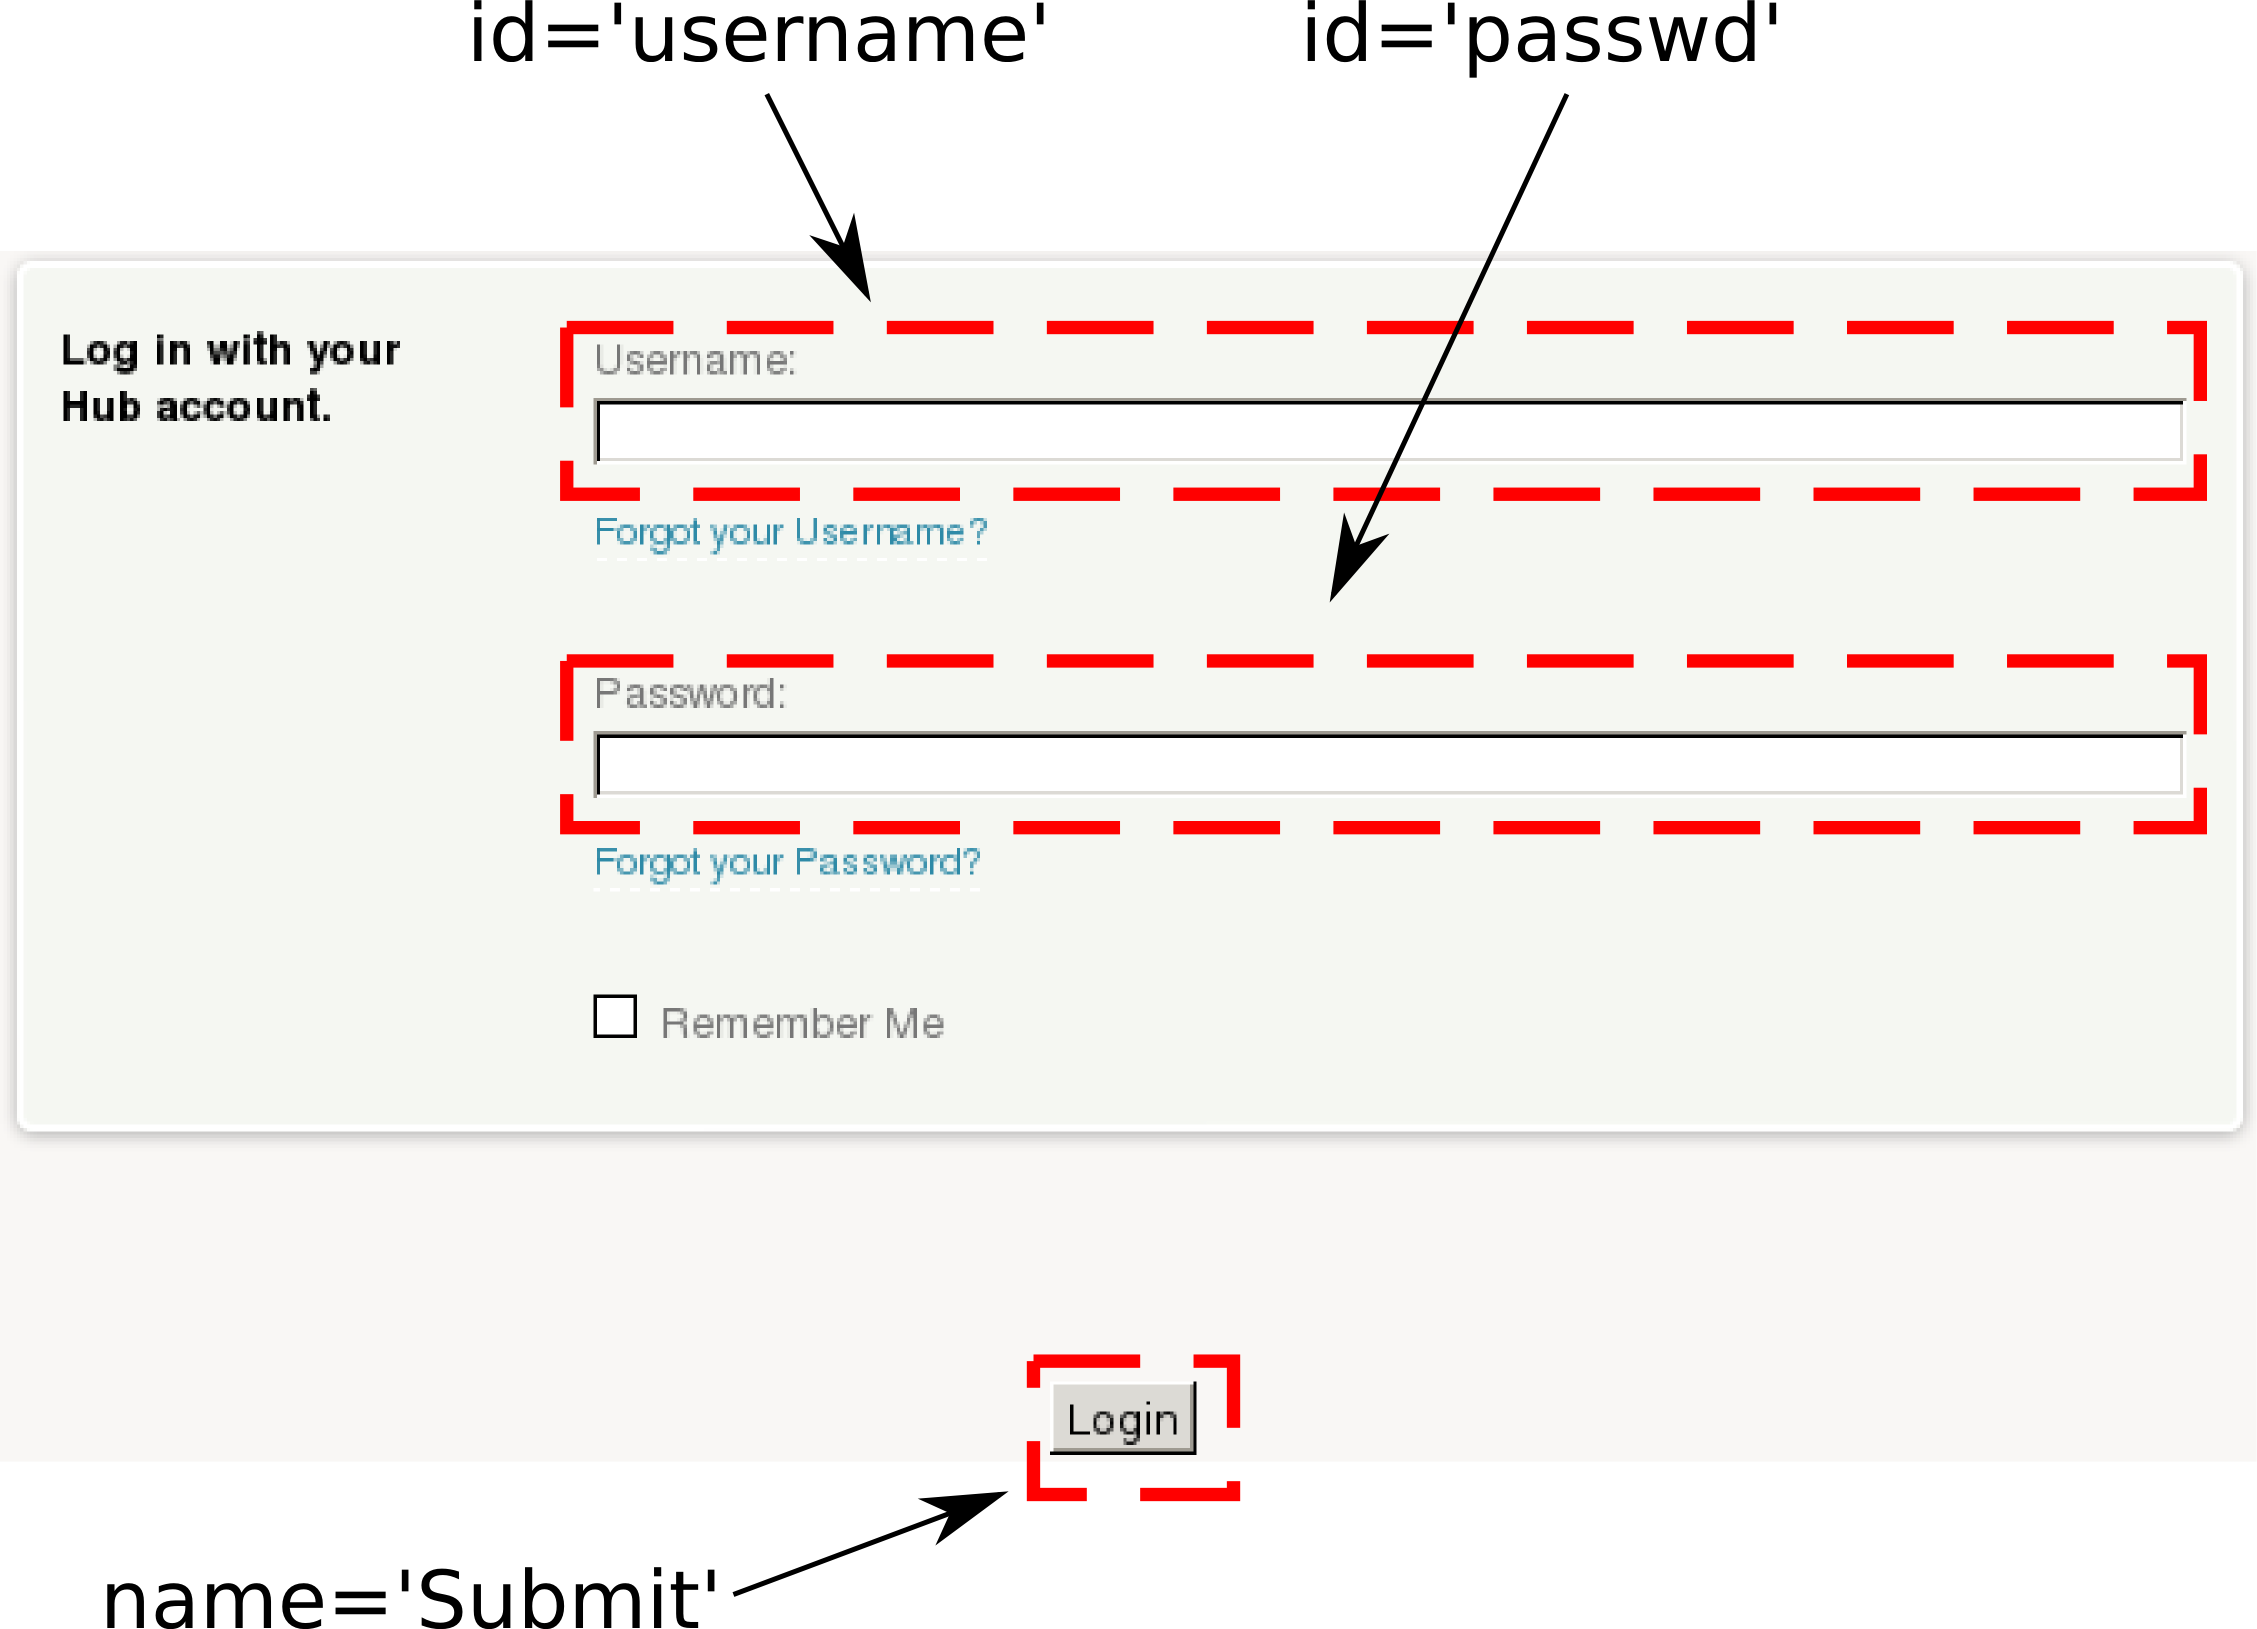
\includegraphics[width=\textwidth]
                  {../../images/hubzero_login_form_with_locators.png}
                \caption{ hubzero.org login form. }
                \label{fig:login_form_with_locators_hubzero}
        \end{subfigure}
        \begin{subfigure}[b]{0.4\textwidth}
                \centering
                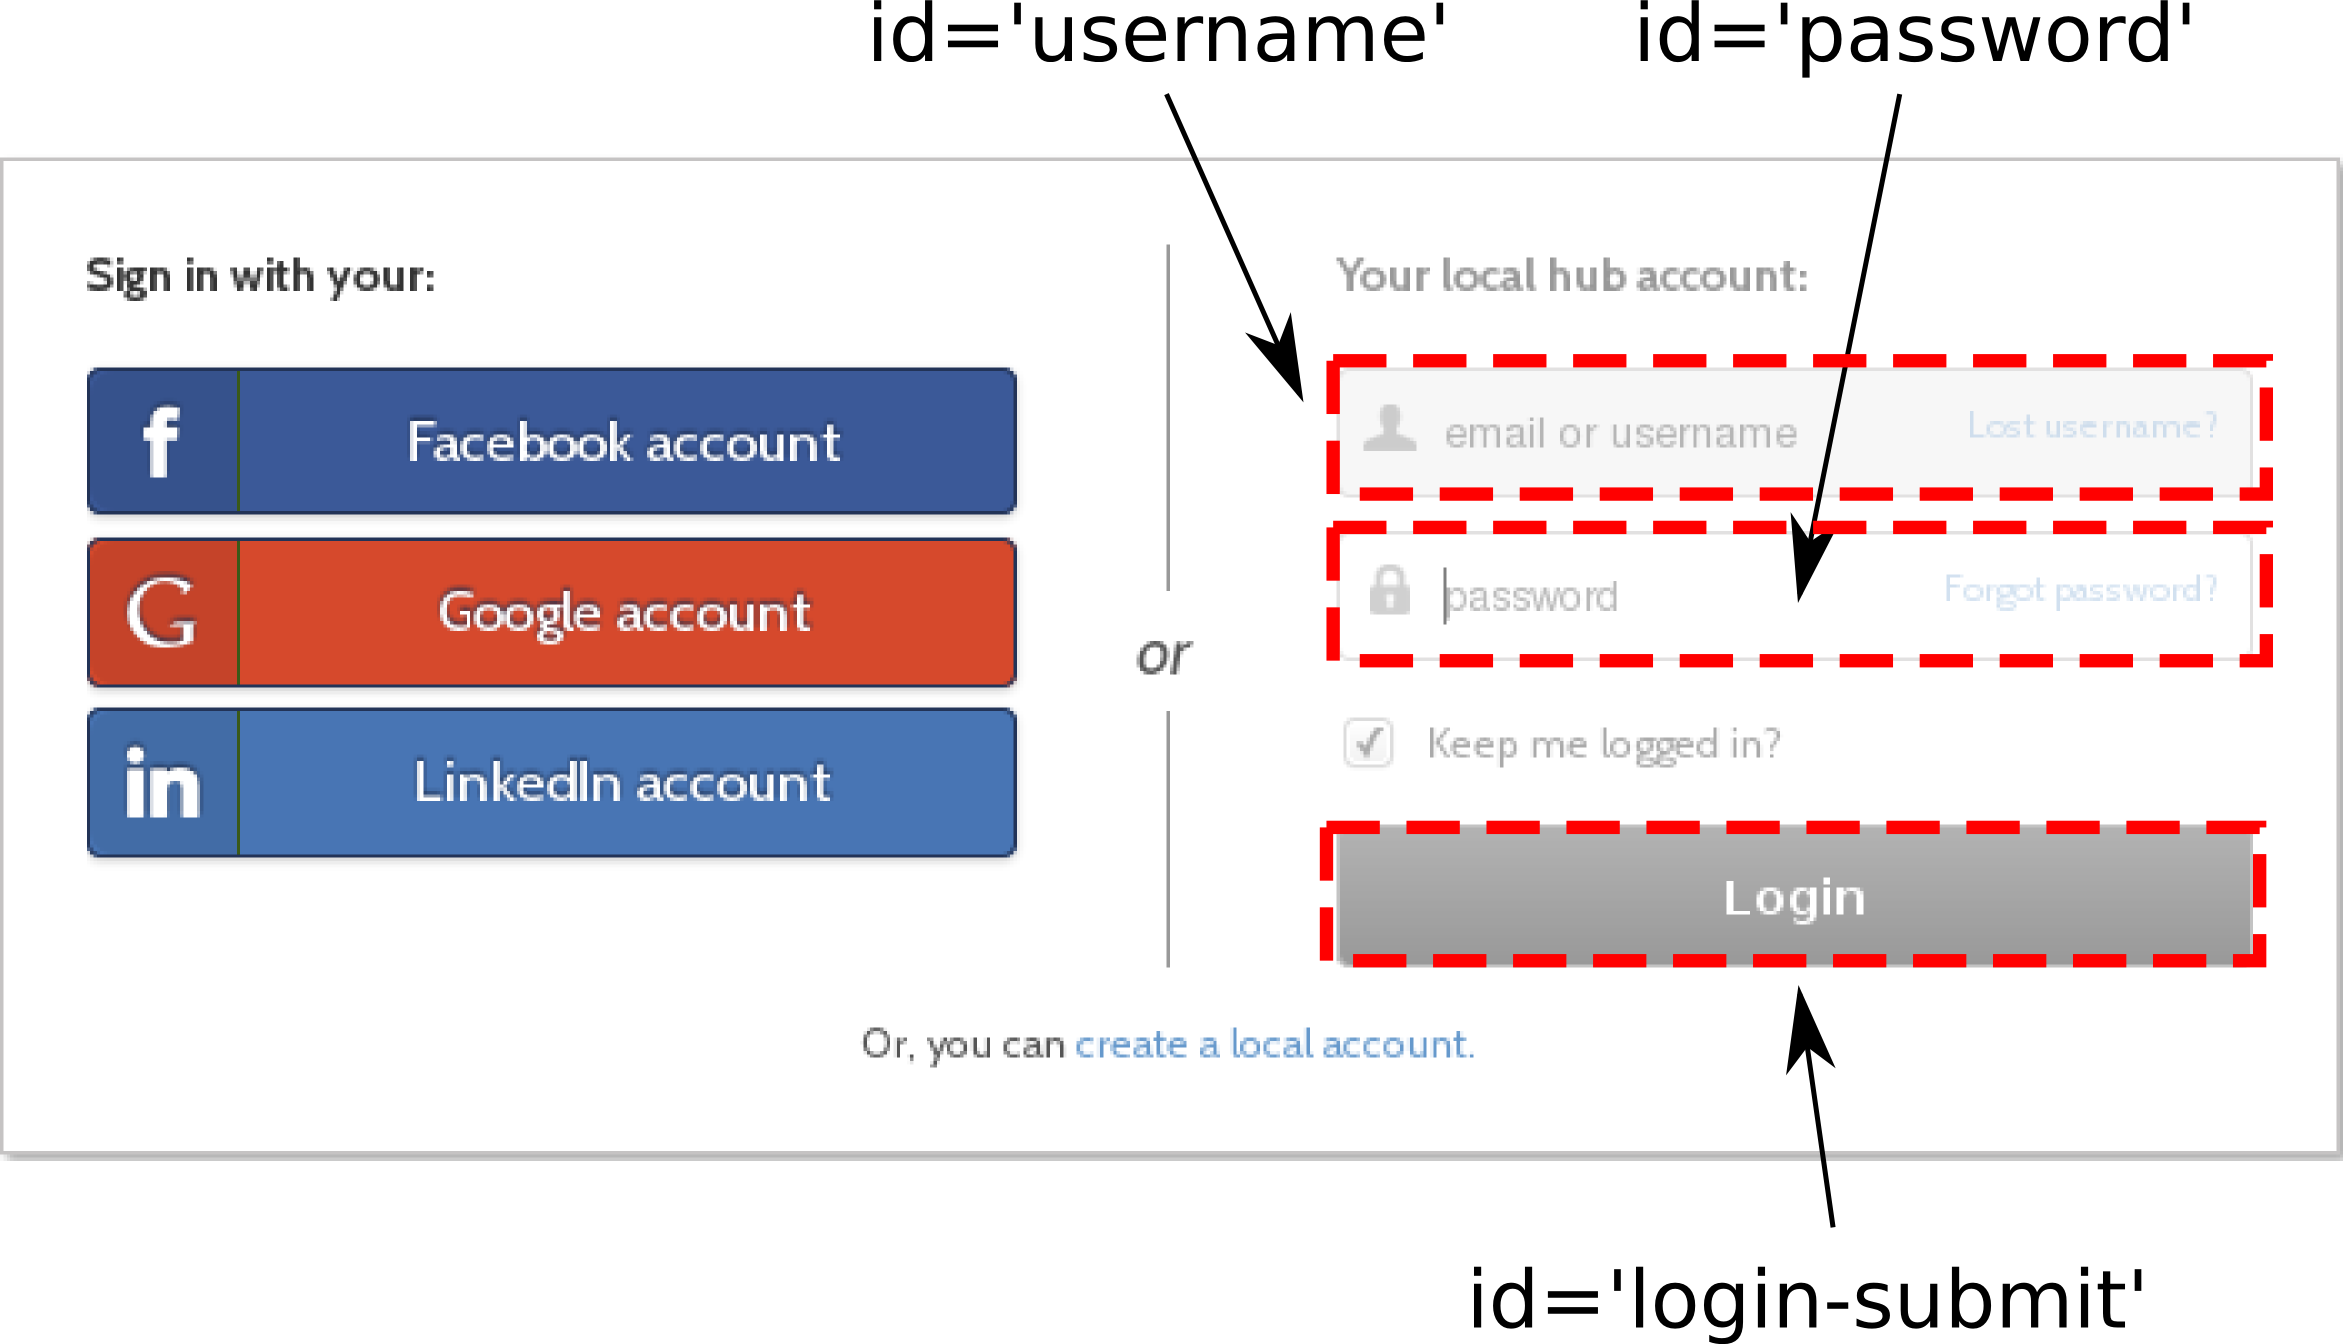
\includegraphics[width=\textwidth]
                  {../../images/nanohub_login_form_with_locators.png}
                \caption{ nanohub.org login form. }
                \label{fig:login_form_with_locators_nanohub}
        \end{subfigure}
        \caption{The variation in locators used on the hub login page causes an
                 additional level of complexity when trying to develop automation
                 scripts generic enough to work across the hubs managed by the
                 HUBzero team.}
        \label{fig:login_form_locators}
\end{figure}

With every new hub the automation script is taken to, there is the opportunity
for either of the previous element locator sets to be used, or even a new set.
Keeping separate automation scripts for each hub is a good way to encourage
divergence of the source. Instead the script should be written in a way where
the differences are abstracted away. This is one of the goals of the Page
Object design pattern.

\begin{xcode}{%
  language=Python,%
  label=lst:login_page_pageobject,%
  caption={Page object for the hub /login page}%
}
# pageobjects.py
locdict = {
  'hubzero' : {
    'username' : '#username',
    'password' : '#passwd',
    'login_b'  : "[name='Submit']"
  },
  'nanohub' : {
    'username' : '#username',
    'password' : '#password',
    'login_b'  : '#login-submit'
  }
}

class LoginPage(object):
    def __init__(self,browser,hub):
        self.username = \
            browser.find_element_by_css_selector(locdict[hub]['username'])
        self.password = \
            browser.find_element_by_css_selector(locdict[hub]['password'])
        self.login_b = \
            browser.find_element_by_css_selector(locdict[hub]['login_b'])

    def login_as(self,username,password):
        self.username.clear().send_keys(username)
        self.password.clear().send_keys(password)
        self.login_b.click()
\end{xcode}

\Cref{lst:login_page_pageobject} shows an example page object for the
hub login page that can be configured to work with hubzero.org or nanohub.org.
The \xfparameter{locdict} variable holds dictionaries of locators that are used by
the \xfclass{LoginPage} class. The user specifies which hub locators they want
to use in the \xfclass{LoginPage} constructor.


\begin{xcode}{%
  language=Python,%
  label=lst:hubzero_login_with_pageobjects,%
  caption={Login automation script for hubzero.org, using page objects}%
}
from selenium import webdriver
from pageobjects import LoginPage

# start the browser and navigate to the login page
browser = webdriver.Firefox()
browser.get('https://hubzero.org/login')

# perform the login action
po = LoginPage(browser,hub='hubzero')
po.login_as(username="testuser",password="abc123")
\end{xcode}


In line 9 of \Cref{lst:hubzero_login_with_pageobjects}, the page object
is created and configured to use the \xflocfam{hubzero} locators. Next, the
automation script calls the page object's \xfmethod{login\_as()} method to
perform the login service on the page.

The page object solution is flexible and robust, allowing the developer to
update the page object to handle more hubs by adding locators to the
\xfparameter{locdict} variable. The new automation script can easily be configured
to work on nanohub.org, or any other hub recognized by the page object.
Additionally, all of the code to perform the login action is in one place, the
\xfmethod{login\_as()} method. If there is a change to how the login service
works, an update to the \xfmethod{login\_as()} method updates all of the scripts
that use the method. The HUBcheck library provides classes for popular HTML
elements to help developers quickly build page objects. Let's explore how to
rebuild the LoginPage page object by using the HUBcheck library.



\section{Rebuilding the Login Page Object With HUBcheck}
\label{sec:rebuilding_login_page_object_with_hubcheck}
% web pages can be thought of as elements and actions
% elements are the pieces you would like to interact with
% actions are the services the web page can perform for you.
% actions are generally a collection of interactions with elements.
% consider the hub login page.
% The hub login page has 



%HUBcheck page objects build upon the idea of dynamically loading page objects
%as a part of the object's configuration. While the HUBzero team supports over
%twenty hubs, the hub configurations can be narrowed down to about three or four
%sets of locators for most page objects. The majority of the variation in
%locators is due to hub software versioning or template differences between
%hubs.
%
%\subsubsection{HUBcheck Page Object base classes}
%
%HUBcheck provides two base classes for creating page objects, the
%\textit{BasePageObject} class and the \textit{BasePageWidget} class. New page
%object classes can be derived from the \textit{BasePageObject} class and
%constructed by combining together multiple \textit{BasePageWidget} objects.
%The \textit{BasePageObject} class allows developers to provide an API for the
%services available on a web page, while the incorporated
%\textit{BasePageWidget} classes perform the work of completing the actions
%associated with the services.
%
%% FIXME: need to add info on what the BasePageObject and BasePageWidget classes
%% are BasePageObject is a container for BasePageWidgets
%
%\subsubsection{Building a Page Object using the BasePageWidget class}

Before representing a web page as a page object, the developer must understand
the purpose of the web page.  Web pages provide services. When a user navigates
to a web page, they are either receiving information from the system
or providing information to the system.  On the hub, the login web page provides
four services. The most recognized service is providing user authentication for
accessing personalized and restricted material on the hub. The other services
provided by the page are to guide users to the registration page, the username
reminder page, and the password reset page.

\begin{figure}[tbh]
  \centering
  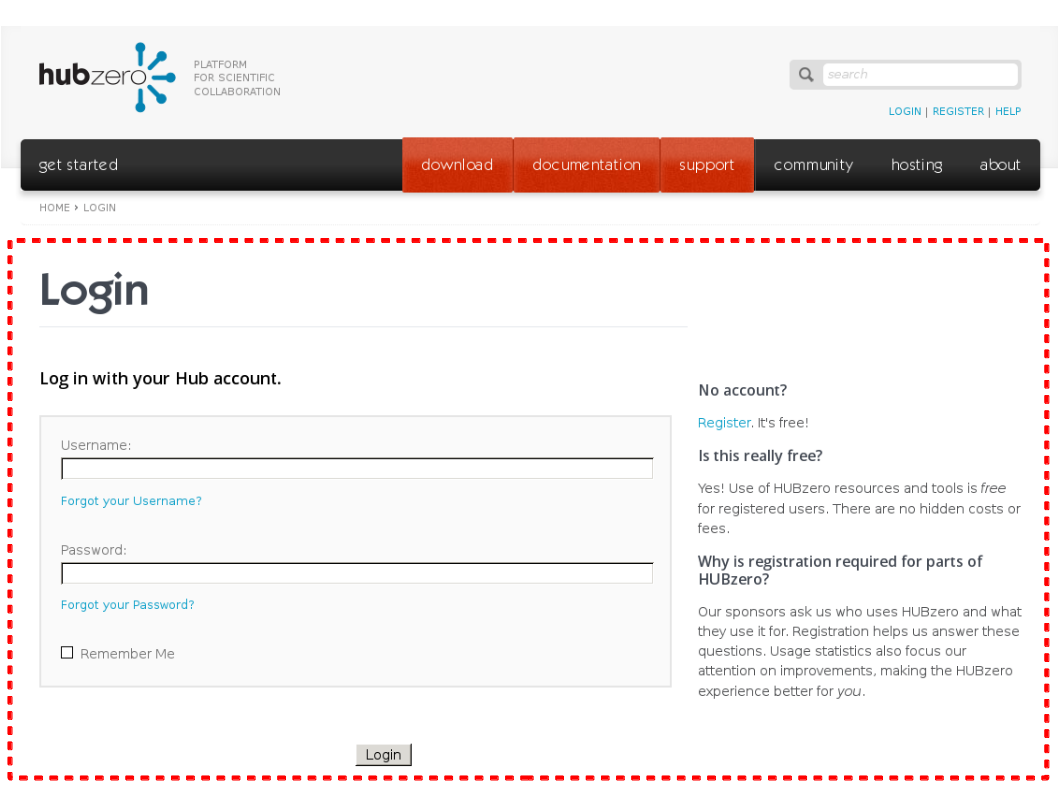
\includegraphics[width=0.75\textwidth]
    {../../images/annotated/hubzero_login_page_parts.png}
  \caption{ The part of the web page represented by the Login widget is outlined in red. }
  \label{fig:hubzero_login_page_parts}
\end{figure}

The login web page can be split into three sections. The header section is the
top portion of the page available on all hub web pages. This includes site
navigation links and banners. The footer section is the bottom portion of the
page, also available on all hub web pages. This section includes copyright,
contact, and site ownership information. The rest of the page can be considered
the Login widget, and is shown in \Cref{fig:hubzero_login_page_parts}.
The Login widget is a mega widget, a widget made up of smaller widgets or
elements, like links, text boxes, checkboxes, and buttons. Each of these elements
are widgets in their own right, and the classes that represent them provide a
few specialized services.

\subsection{Matching Web Page Widgets to HUBcheck Page Object Classes}
\label{ssec:matching_widgets_to_page_objects}

\begin{figure}
        \centering
        \begin{subfigure}[b]{0.5\textwidth}
                \centering
                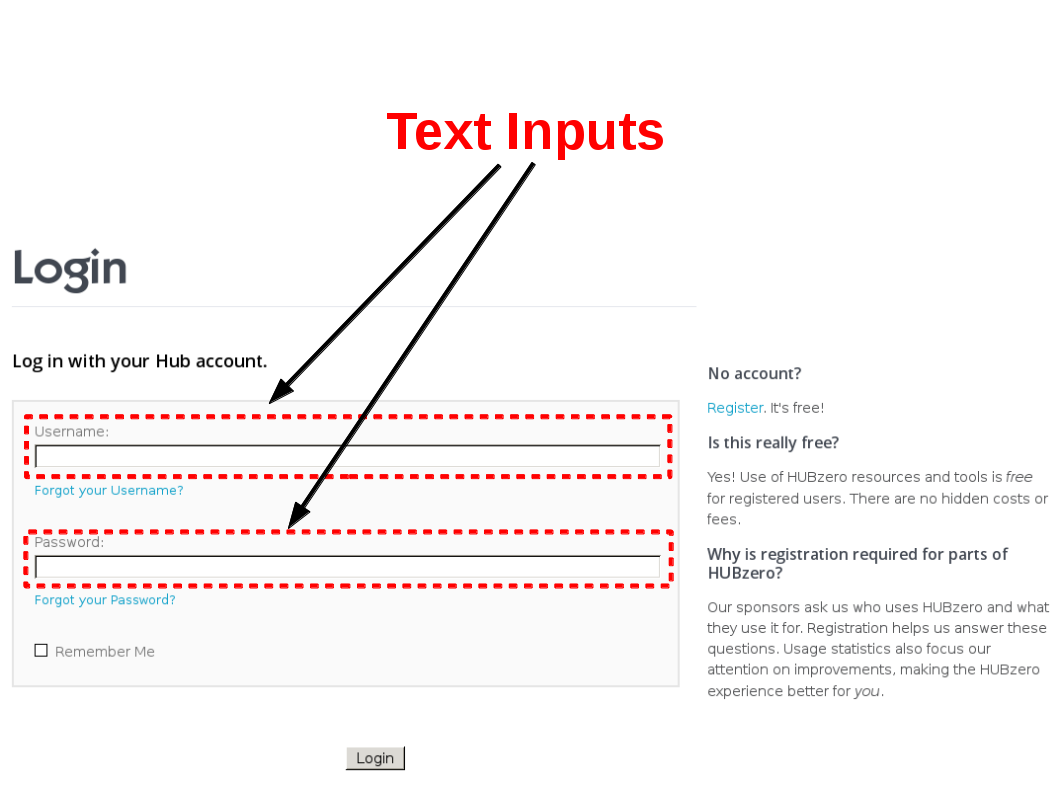
\includegraphics[width=\textwidth]{../../images/annotated/hubzero_login_page_textbox.png}
                \caption{Text box widgets}
                \label{fig:login_page_text_boxes}
        \end{subfigure}
        \begin{subfigure}[b]{0.5\textwidth}
                \centering
                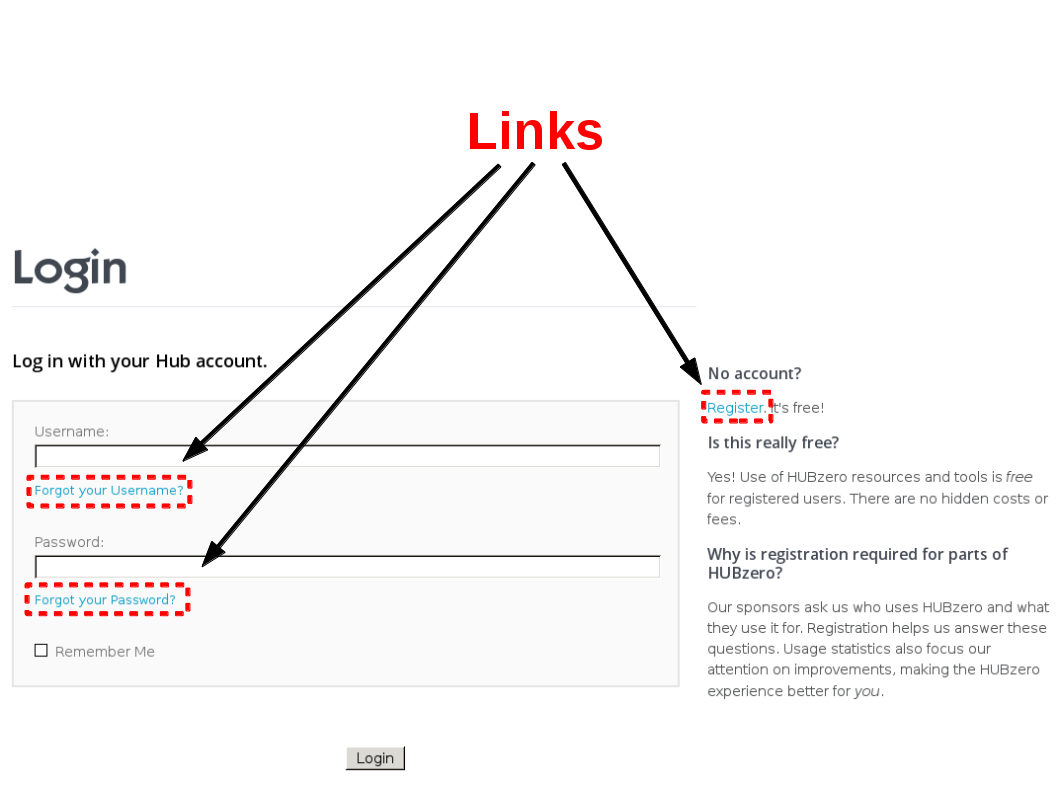
\includegraphics[width=\textwidth]{../../images/annotated/hubzero_login_page_links.png}
                \caption{Link widgets}
                \label{fig:login_page_links}
        \end{subfigure}
        \begin{subfigure}[b]{0.5\textwidth}
                \centering
                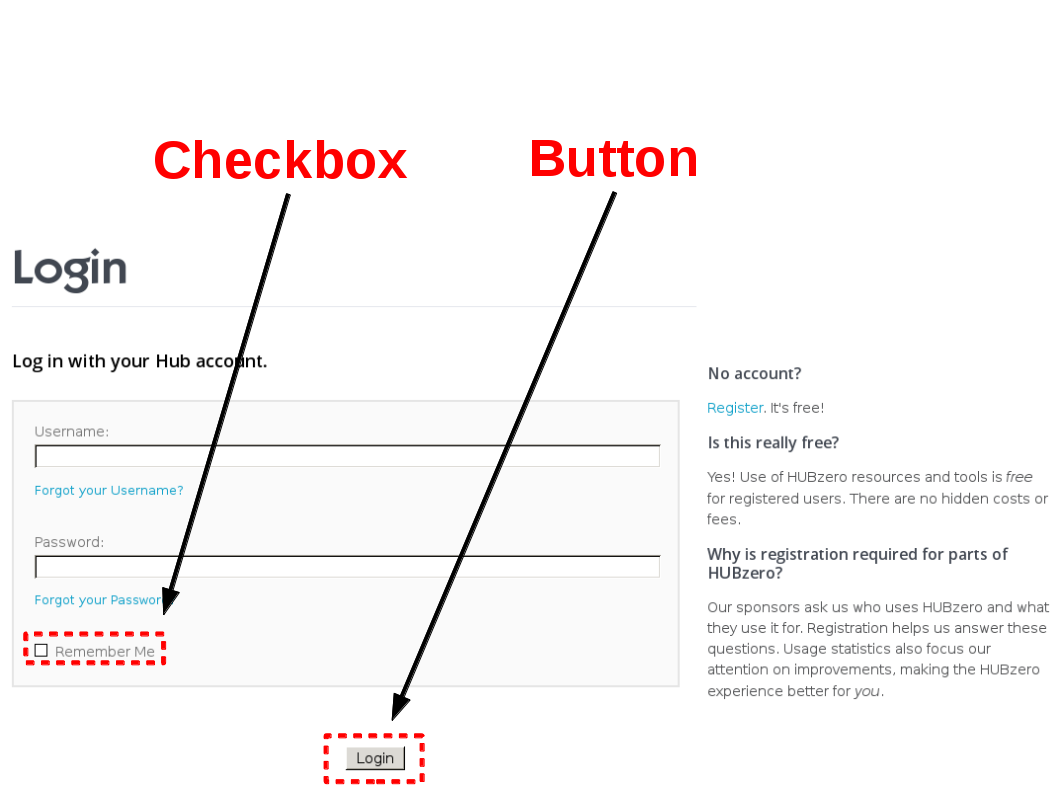
\includegraphics[width=\textwidth]{../../images/annotated/hubzero_login_page_cb_button.png}
                \caption{Checkbox and Button widgets}
                \label{fig:login_page_cb_button}
        \end{subfigure}
        \caption{The login web page is made up of several types of widgets.}
        \label{fig:login_page_widgets}
\end{figure}

On the login page, each element can be represented by a HUBcheck page object
class. Links are represented by the \xfclass{Link} class, input text boxes are
represented by the \xfclass{Text} class, checkboxes are represented by the
\xfclass{Checkbox} class, and buttons are represented by the \xfclass{Button}
class.  \Cref{lst:login_page_data_members} starts to build a new
\xfobject{Login} page object by identifying the widgets that are available on
the web page and matching them up with comparable HUBcheck classes.  In the
code, the username and password text boxes are represented by \xfobject{Text}
objects. The username reminder, password reset, and register links are
represented by \xfobject{Link} objects. The remember me checkbox is represented
by a \xfobject{Checkbox} object and the form submission button is represented
by a \xfobject{Button} object.  HUBcheck includes nine classes that represent
popular HTML elements including \xfclass{Button}, \xfclass{Checkbox},
\xfclass{Link}, \xfclass{Radio}, \xfclass{Select}, \xfclass{Text},
\xfclass{TextReadOnly}, \xfclass{TextAC}, \xfclass{TextArea}, and
\xfclass{Upload}.

\begin{xcode}{%
  language=Python,%
  label=lst:login_page_data_members,%
  caption={The Login class is a composition of other classes representing the %
           elements on the web page.}%
}
class Login(BasePageWidget):
    def __init__(self):
        ...
        self.username  = Text(self,{'base':'username'})
        self.password  = Text(self,{'base':'password'})
        self.remember  = Checkbox(self,{'base':'remember'})
        self.remind    = Link(self,{'base':'remind'})
        self.reset     = Link(self,{'base':'reset'})
        self.register  = Link(self,{'base':'register'})
        self.submit    = Button(self,{'base':'submit'})
        ...
\end{xcode}

The \xfclass{Login} page object has methods that mirror the services offered by
the login web page. These methods abstract away the steps required to perform
the service and reduce the service to a single call to the page object's API.
\Cref{lst:login_page_member_functions} declares four methods that
correspond to the services provided by the login page, including
\xfmethod{login\_as()}, \xfmethod{goto\_remind()}, \xfmethod{goto\_reset()},
and \xfmethod{goto\_register()}.

\begin{xcode}{%
  language=Python,%
  label=lst:login_page_member_functions,%
  caption={The Login object's methods match the services provided by  %
            the widget.}%
}
class Login(BasePageWidget):
    ...
    def login_as(self,username,password):
        self.username.value = username
        self.password.value = password
        self.submit.click()
    def goto_remind(self):
        self.remind.click()
    def goto_reset(self):
        self.reset.click()
    def goto_register(self):
        self.register.click()
\end{xcode}


Inside the methods, page object data members representing the web page elements
take over to do the real work of typing values into the login form's fields,
clicking links or buttons, and toggling checkboxes. For the
\xfmethod{login\_as()} method, the \xfparameter{self.username} and
\xfparameter{self.password} objects are responsible for updating the username
and password fields on the web page by using the method's arguments as inputs.
\xfparameter{self.username} and \xfparameter{self.password} are both instances
of the \xfclass{Text} class, with a \xfparameter{value} property which acts as
an accessor, allowing users to query or set the current value of the field on
the web page. In line 4 of \Cref{lst:login_page_member_functions},
\xfparameter{self.username}'s \xfparameter{value} property is assigned a new
value. This assignment causes a Selenium WebDriver handle for the text input
field to be retrieved from the web page's HTML DOM.  The text input field is
cleared of any previous value, and the new value is written to the field on the
web page. This happens again, in line 5, for the \xfparameter{self.password}
object. Lines 9 - 12 of \Cref{lst:text_widget_value_property} show the
sequence of events in more detail.

\begin{xcode}{%
  language=Python,%
  label=lst:text_widget_value_property,%
  caption={The Text object manages finding and writing to the Selenium  %
            WebDriver object handle.}%
}
class Text(BasePageWidget):
    @property
    def value(self):
        e = self.owner.find_element_in_owner(self.locator)
        return e.get_attribute('value')

    @value.setter
    def value(self, val):
        e = self.owner.find_element_in_owner(self.locator)
        e.click()
        e.send_keys(Keys.CONTROL,'a')
        e.send_keys(val)
\end{xcode}

\subsection{Specifying Element Locators for Page Object Classes}
\label{ssec:specifying_page_object_element_locators}

The \xfclass{Login} page object is almost complete. In
\Cref{lst:login_page_data_members}, we specified the elements available on the
login web page. In \Cref{lst:login_page_member_functions} we added
functions to fulfill all of the services offered by the web page. The next step
is to specify the locators for the web page elements.

HUBcheck page object classes have a complementary set of
locator classes that specify sets of element
locators. \Cref{lst:login_page_object_locators} shows two example
locator classes for the hubzero.org and nanohub.org login pages discussed in
\Cref{sec:review_page_object_design_pattern}.

\begin{xcode}{%
  language=Python,%
  label=lst:login_page_object_locators,%
  caption={Locators for the Login page object}%
}
class Login_Locators_Base_1(object):
    locators = {
        'username'  : "css=#username",
        'password'  : "css=#passwd",
        'submit'    : "css=[name='Submit']",
        ...
    }

class Login_Locators_Base_2(object):
    locators = {
        'username'  : "css=#username",
        'password'  : "css=#password",
        'submit'    : "css=#login-submit",
        ...
    }
\end{xcode}

Each locator class holds a dictionary of locators that is dynamically loaded by
the page object class during initialization and is used to override the
locators of its data members.  In \Cref{lst:login_page_data_members},
the \xfparameter{self.submit} data member is instantiated with the dictionary
\xfinlinecode{\{`base': `submit'\}} as one of the arguments. This is a locator
override, which maps the \xfinlinecode{`base'} locator inside of the
\xfparameter{self.submit} object to the value of the \xfinlinecode{`submit'} locator of
the \xfclass{Login} page object. The value of the \xfinlinecode{`submit'} locators is
dynamic because it depends upon which locator class is loaded by the page
object, \xfclass{Login\_Locators\_Base\_1} or \xfclass{Login\_Locators\_Base\_2}.

The pattern of separating locators from the page object allows HUBcheck page
objects to be used across multiple hubs. When new hubs are created new locators
can be added to the system, if needed, leaving the page object classes
untouched. More often then not, new hubs use locators that have already been
added to the HUBcheck library.  When new versions of the HUBzero software are
released, the locators also can be added to the HUBcheck library without
modifying the existing page objects. In the next section, we dive deeper into
patterns that can be used to build page objects. While these patterns can be
found throughout the HUBcheck library, they include ideas that are best
practices for building all kinds of page objects.


\section{Incorporating Classic Design Patterns into Page Objects}
\label{sec:incorporate_design_patterns_into_page_objects}

The social aspect of the hub website encourages members to contribute content
and organize in communities. To do this, the user must interact with hub web
pages containing web forms, evaluate search results represented as lists or tables,
and upload content. These three forms of interaction often show up in the web
components built for the hub, and by extension, in the page objects built to
interface with those web components.

For most web pages, identifying the widgets and services for the page is
straight forward. For other web pages, the widgets are not so obvious and
inefficient solutions can lead to bad interfaces that add work for developers
instead of reducing work. Three types of interactions found on the hub fall
into this latter group of web pages: using web forms, reading lists
of data, and interacting with items in iframes.

In this section, we'll introduce three patterns, the WebForm pattern,
the ItemList pattern, and the IframeWrap pattern, that can be
used to quickly produce page objects that work with components that ask the
user to interact through web forms, lists of items, or through an iframe.


\subsection{WebForm Pattern}
\label{ssec:webform_pattern}

Web forms are ubiquitous across the web. They are the best way to collect
information from the user, so there is no wonder why they are a part of many
hub web components. On the hub, users experience them as a part of larger
processes to create, update, or delete content. Interacting with most web forms
takes place in two phases, population and submission.  The first phase,
populating the form, involves searching for fields in the form and assigning
them values. The second phase, submitting the form, simply involves clicking
the submit button on the form.

Many of the harder to test aspects of a hub's web site involve working through
multi-step processes that often include web forms. The novice approach to
creating page objects for these web forms can lead to unintuitive interfaces.
The hub login page and new support ticket page are classic examples of web
forms. When evaluated separately, the interfaces may seem very different.
Certainly the services provided by the pages are different and so are the
fields that need to be populated, but these things can be considered
configuration steps for a class that tackles the larger problem of form
population and submission.

\begin{figure}[tbh]
  \centering
  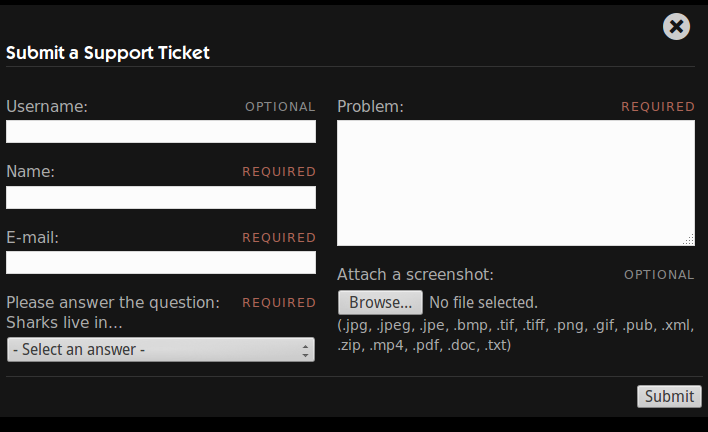
\includegraphics[width=0.75\textwidth]
    {../../images/hubzero_dropdown_support_ticket_form.png}
  \caption{ Testing the hubzero.org support ticket form. }
  \label{fig:hubzero_dropdown_support_ticket_form}
\end{figure}

% show the support ticket page
% explain that usual way to interact with the support ticket page is to
% create a page object with a bunch of accessor methods for setting fields
% on the web page. the last thing to do is click the submit button.
% this approach makes the developer have to lookup all of the accessor methods
% for the page object and makes reading the inputs for the form hard to read.
% the proposed interface stores the 


\begin{xcode}{%
  language=Python,%
  label=lst:trouble_report_form_po_interface_1,%
  caption={The typical interface for a web form requires the automation %
           developer to call page object accessors to populate the form.}%
}
po = TroubleReportForm()

po.set_name('testuser')
po.set_email('tu@hubzero.org')
po.set_problem('test problem')
po.set_upload('myscreen.png')

po.submit.click()
\end{xcode}

The typical page object interface for a web form requires the automation
developer to call page object accessor methods to populate each field of a
form. Using accessor methods provides a clean interface for the populate phase.
An alternative approach is to pass the form inputs to a single method, and
allow the method to perform the form population. Similarly, for submitting a
web form, a single method can be used to populate and submit the form. This is
the idea behind the WebForm pattern.
\Cref{lst:trouble_report_form_po_interface_2} shows an example of the interface.


%  caption={The proposed interface for a web form utilizes two methods,
%           \textit\{populate\_form()\} to handle filling in the form inputs,
%           and \textit\{submit\_form()\} to handle form submission.}%
\begin{xcode}{%
  language=Python,%
  label=lst:trouble_report_form_po_interface_2,%
  caption={An example interface for a web form utilizing two methods, %
           populate\_form() to handle filling in the form inputs, %
           and submit\_form() to handle form submission.}%
}
po = TroubleReportForm()

data = {
  'name'    : 'testuser',
  'email'   : 'tu@hubzero.org',
  'problem' : 'test problem',
  'upload'  : 'myscreen.png'
}

po.populate_form(data)

po.submit_form()
\end{xcode}


The purpose of the WebForm pattern is to help standardize the interface for
filling out web forms.  The usual interface makes the script writer work hard
to remember the accessor methods for the inputs on the form. The WebForm
pattern encourages the automation developer to organize the inputs for the form
and send the inputs to a standard page service, the \xfmethod{populate\_form()}
method. Later the user can submit the form using another standard service, the
\xfmethod{submit\_form()} method. These two services are supported for all
forms.

Implementing the WebForm pattern requires a page object that represents a web
form to be derived from an abstract base class that provides the
\xfmethod{populate\_form()} and \xfmethod{submit\_form()} methods.
\Cref{lst:web_form_pattern_formbase} shows an example of such a class.


%While the
%page provides a number of services, the most often used service is the web
%form. The page object from
%\Cref{sec:rebuilding_login_page_object_with_hubcheck} performs both phases the
%population and submission phases of web form interaction in the
%\textit{login\_as()} method, but it could be rewriten to expose these two
%independent actions seperately and provide an easy to read interface that is
%common to all web forms by using the \textit{WebForm} pattern.

%The WebForm pattern provides a standard way to automate the
%interaction with web forms. The class that implements the pattern would need a
%way to accept information regarding the available fields of the web form. The
%two phases can be considered services of the web page, and implemented as
%methods of the class. Page objects could then be derived from this class to get
%the standard interface for a web form. An example class is shown in
%\Cref{lst:web_form_pattern_formbase}.

\begin{xcode}{%
  language=Python,%
  label=lst:web_form_pattern_formbase,%
  caption={\xfclass{FormBase} is an example base class for web forms}%
}
class FormBase(BasePageWidget):
    def __init__(self, owner, locatordict={}):
        ...
        self.submit = Button(self,{'base':'submit'})

    def populate_form(self, data):
        for (k,v) in data:
            widget = getattr(self,k)    # find the widget
            widget.value = v            # set its value

    def submit_form(self,data=[]):
        self.populate_form(data)
        return self.submit.click()
\end{xcode}

In \Cref{lst:web_form_pattern_formbase}, the \xfclass{FormBase} class provides
a submit button object in the constructor, and relies on the derived class to
supply the fields of the form as data members. The two services of the web
form, populating the form and submitting the form, are performed by the class's
\xfmethod{populate\_form()} and \xfmethod{submit\_form()} methods.

\begin{figure}[tbh]
  \centering
  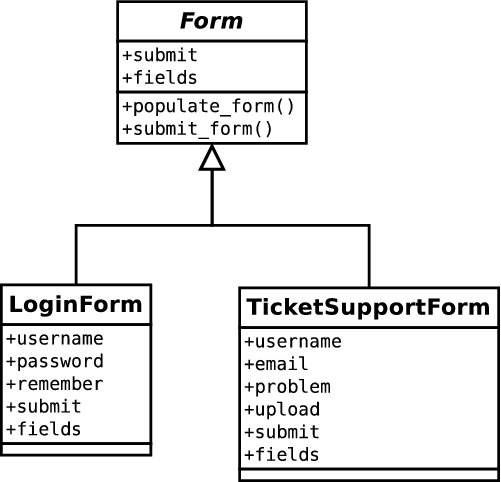
\includegraphics[width=0.50\textwidth]
    {../../diagrams/webform_pattern.png}
  \caption{ In the WebForm pattern, the \xfclass{FormBase} base class
            provides the two services essential to all web forms,
            populating the form and submitting the form. }
  \label{fig:webform_pattern_class_diagram}
\end{figure}

The \xfclass{FormBase} class can be applied to the hub login page example from
\Cref{sec:rebuilding_login_page_object_with_hubcheck} just as easily as it can
be applied to the new support ticket page from
\Cref{fig:hubzero_dropdown_support_ticket_form}, they are both web forms after
all.  To build a new page object for the login page, the first step is to
subclass \xfclass{FormBase} and add the form's fields to the new class's
constructor.  \Cref{lst:web_form_pattern_login_page} shows what the new
page object class would look like.

\begin{xcode}{%
  language=Python,%
  label=lst:web_form_pattern_login_page,%
  caption={An example page object for the hub login page, using \xfclass{FormBase}}%
}
class LoginPage(FormBase):
    def __init__(self, owner, locatordict={}):
        super(LoginPage,self).__init__(owner,locatordict)
        ...
        self.username = Text(self,{'base':'username'})
        self.password = Text(self,{'base':'password'})
        self.remember = Checkbox(self,{'base':'remember'})
\end{xcode}

The new LoginPage class is derived from the FormBase class.  In the LoginPage
constructor, we add data members for the fields of the login page's form, the
username field, the password field, and the remember checkbox. That's it!
Users can interact with the LoginPage page object by supplying the values for
the fields as a dictionary or a list of tuples to either of the inherited
service methods, \xfmethod{populate\_form()} or \xfmethod{submit\_form()}, and
the service methods take care of inspecting the LoginPage object for the
widgets.


\begin{xcode}{%
  language=Python,%
  label=lst:web_form_pattern_using_login_po,%
  caption={Interacting with the new LoginPage page object}%
}
form_data = {'username' : 'testuser',
             'password' : 'abc123',
             'remember' : False}
po = LoginPage()
po.populate_form(form_data.items())
po.submit_form()
\end{xcode}

Using the WebForm pattern simplifies building web form page objects to a single
step of declaring the fields of the form. There are several variations of the
FormBase class, including those that fill out forms in a specified order,
validate inputs, or have extra HTML buttons like cancel or preview. These
variations can usually be accommodated by adjusting the derived class or the
data structures being passed to the base class's service methods.


\subsection{ItemList Pattern}
\label{ssec:itemlist_pattern}

%
% Used to quickly build page objects for web pages that repeatedly list items
% of the same type.
%
% Examples include:
%   1. list of search results.
%   2. table of items.
%
% Real Example: Contribtool Tools Pipeline
%
%

% \subsection{Pattern Name and Classification:}
%
%   ItemList Pattern
%   Purpose: Creational - we are defining a good way to dynamically create
%                         a page object to describe and access a specific
%                         item in a list of items.
%   Scope: Object
%


%\subsection{Intent}

Lists of items on web pages are often built dynamically, pulling information
from databases to present the user with up-to-date information. The
amorphous nature of a web page with a dynamically generated list makes it hard to
build a static page object to represent it. Since the number of items in the
list may fluctuate, it cannot be hard coded into the page object.  Even if it
could, creating individual page objects for each row/item in the list at once
may be memory and time intensive.

Lists of items are an area where the traditional approach to building page
objects is hard to apply. Without knowing ahead of time the number of items in
the list, static page objects cannot be built with an object representing each
item. Instead of manually creating an object for each item in the list, it is
better to step back and evaluate the ways lists are used. Lists are a quick,
organized way of presenting enumerable pieces of data back to the user. Many
lists hold items that provide an overview of the available data by using text
fields or links to web pages with more details. Other types of lists contain
items that exhibit all available data in a single text field. Regardless of the
way the data is displayed, the information in each item depends upon the type
of list being presented.  Users may interact with a single list item at a time
or they may interact with the list as a whole, accessing list properties like
the item count and searching for specific items.

The ItemList design pattern defines a way to dynamically instantiate a page
object that represents a single, specific item from an arbitrarily sized list
of items. Page objects built using this pattern can be used to access the
properties of the single item it was instantiated for and can be quickly
updated to reference another item in the list. The pattern uses elements of the
Iterator pattern \cite{Gamma:1995:DPE:186897} and Factory Method pattern
\cite{Gamma:1995:DPE:186897}, and introduces the concept of the \textit{locator
template}, a template that has a value substituted into it, to create a new web
page element locator.

% FIXME: check out the description and example for the Flyweight pattern
%        to see if it can be applied to the Item class
%
% template locator idea introduced by Adam Goucher


\begin{figure}[ht!]
        \centering
        \begin{subfigure}[b]{0.75\textwidth}
                \centering
                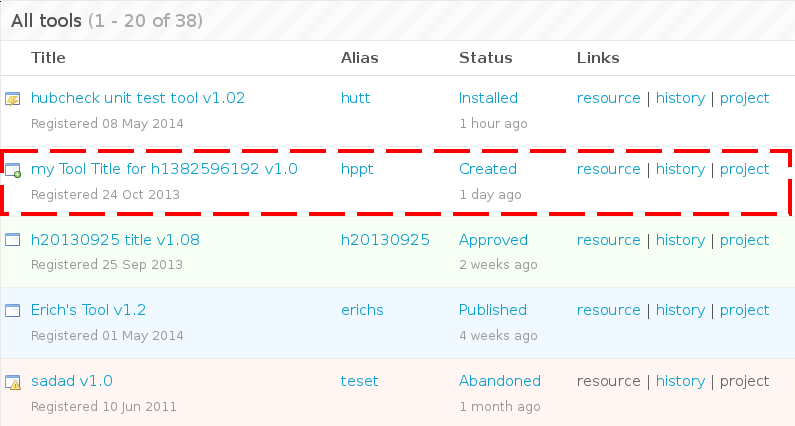
\includegraphics[width=\textwidth]{../../images/hubzero_tool_pipeline_table.png}
        \end{subfigure}
        \begin{subfigure}[b]{0.75\textwidth}
                \centering
                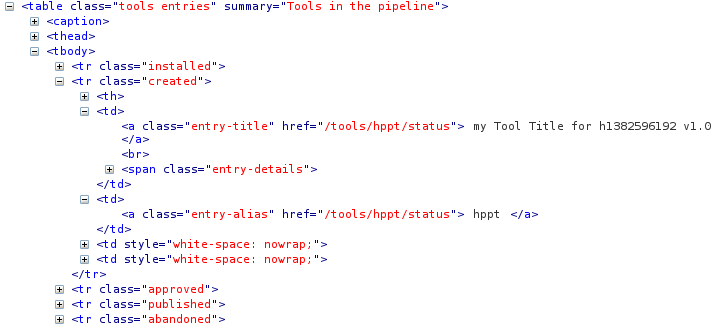
\includegraphics[width=\textwidth]{../../images/hubzero_tool_pipeline_table_html.png}
        \end{subfigure}
        \caption{The hub Tool Pipeline table is a dynamically created list of items.
                 Each row in the table provides links and information regarding a
                 specific simulation tool registered on the hub.}
        \label{fig:itemlist_motivation_tool_pipeline_table}
\end{figure}


In the hub's tool contribution process, the Tool Pipeline, shown in
\Cref{fig:itemlist_motivation_tool_pipeline_table}, is an HTML table that shows
all tools that have been registered on a hub. Each row of the table shows the
tool's title, alias, status, time since the tool was registered, time since the
last status change, and links leading to the tool's resource, status, and
communications history web pages. The Tool Pipeline web page also allows users
to search for specific tools by alias.


Building a page object for a dynamic web page like this is hard because the
information in the table is pulled from a database and may change over time.
While a human user can look at each item quickly to find the item they are
interested in, an automated system must iteratively scan all items until
matching criteria is found. This pattern of listing information from databases
is not unique to the Tool Pipeline page. On the hub, it is also found in the
Tags component when displaying all available tags, in the Support component
when listing support tickets, the Groups component, Questions and Answers,
Projects, Wish List and more.

\begin{figure}[ht!]
        \centering
        \begin{subfigure}[b]{0.45\textwidth}
                \centering
                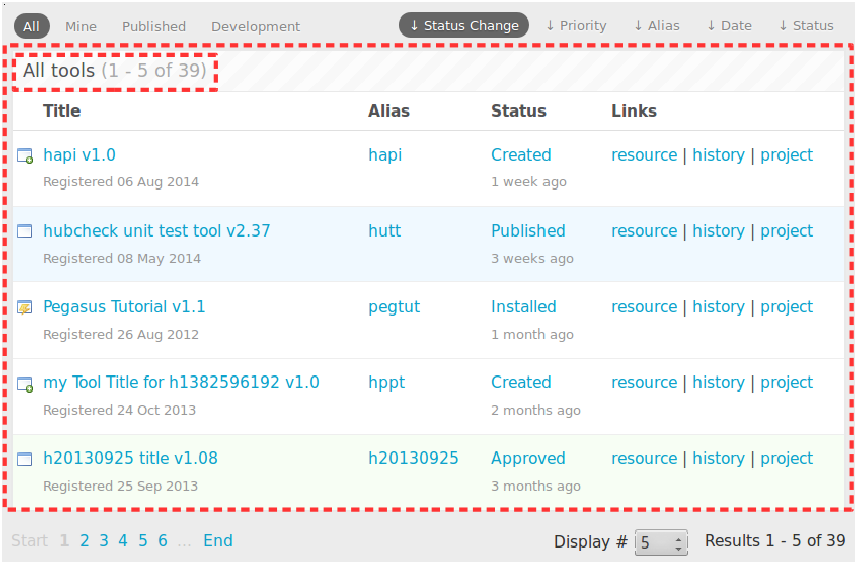
\includegraphics[width=\textwidth]{../../images/item_list_pattern_container.png}
                \caption{Container class coverage}
                \label{fig:itemlist_container_item_imgs_container}
        \end{subfigure}
        \begin{subfigure}[b]{0.45\textwidth}
                \centering
                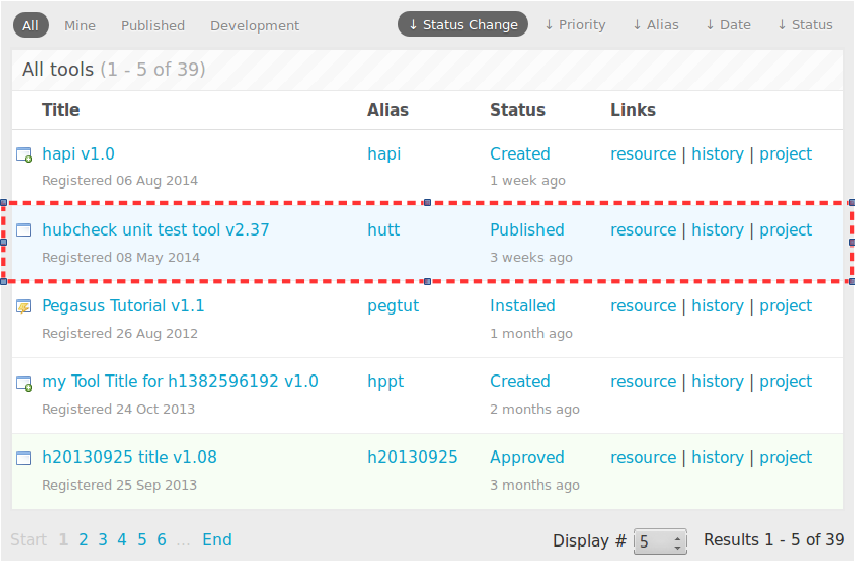
\includegraphics[width=\textwidth]{../../images/item_list_pattern_item.png}
                \caption{Item class coverage}
                \label{fig:itemlist_container_item_imgs_item}
        \end{subfigure}
        \caption{The Container and Item classes are the foundation of the ItemList pattern.}
        \label{fig:itemlist_container_item_imgs}
\end{figure}


The ItemList pattern provides a standard way to describe and traverse items in
a list or table on a web page. The main participants of the pattern are two
base classes, \xfclass{Container} and \xfclass{Item}. The container class
represents the meta-data of the list.  Automation developers can ask the
container questions regarding properties of the list, like \textit{how many
items are in the list?} The container cannot answer questions about specific
items in the list, but can provide access to the list elements, either
sequentially or through a limited search capability. The item class represents
a single item in the list.  Automation developers can query this class for
information about the item it represents in the list. Additionally, the item
class can be updated on the fly to point to another item from the list. The
container and item classes provide interfaces that, when implemented, can be
used to represent lists, tables, and other data structures that appear on the web
page as a collection of items.

\begin{figure}[tbh]
  \centering
  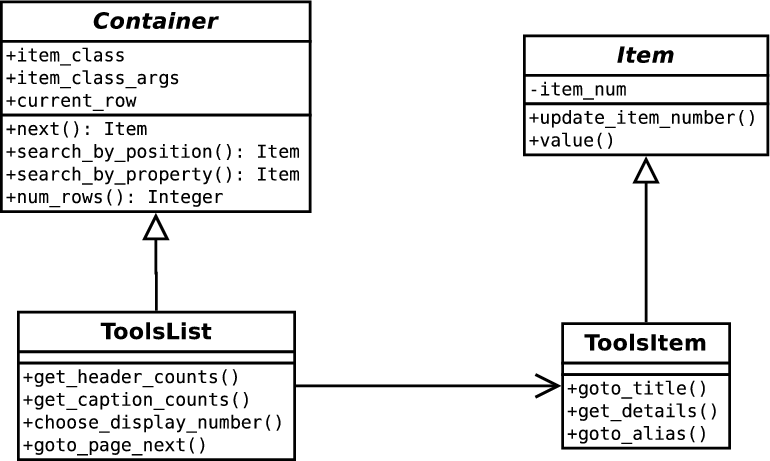
\includegraphics[width=0.75\textwidth]
    {../../diagrams/itemlist_pattern.png}
  \caption{ The ItemList pattern uses a container class to represent the
            list and provide access to list meta-data while providing
            access to elements of the list through an item class. It
            incorporates the Iterator and FactoryMethod patterns. }
  \label{fig:itemlist_pattern_class_diagram}
\end{figure}

%Let's take a closer look at how we can implement a container class. We
%mentioned earlier that the container class should provide access to the list
%meta-data. One of the more frequent queries for the container class asks
%\textit{how many items are in the list?}


%The pattern involves two classes, the Container
%class and the Item class. The Container class describes the properties of the
%list, including decorations like counters that may be at the top or bottom of
%the displayed widget. It also provides ways to access individual items in
%the list which are represented by the Item class. The Item class serves as a
%template for an item in the list. It provides ways to access the properties of
%the specific item in the list that it represents, as well as a way to update
%which item in the list it represents.


%\subsection{Applicability}
%
%Developers should consider using the ItemList pattern when
%
%\begin{itemize}
%\item Information being displayed on the web page can be formed into repeatable items.
%\item The items can be enumerated and iterated over.
%\item The items are dynamically generated and not guaranteed to always exist.
%\end{itemize}
%
%
%% Structure:
%%
%%   (Need a graphical representation of the classes in the pattern)
%
%
%\subsection{Participants}
%
%\subsubsection{Container class}
%
%The Container class represents the list of items as a container or shell.
%Developers can access properties of the list, like counters or the number items
%in the list, through the Container object. Developers can also iterate over the
%items of the list, retrieve an item by position, or retrieve an item by
%property, all of which return an Item object.
%
%\subsubsection{Item class}
%
%The Item class describes the features of a single item in the list. The Item
%object can be used to further query properties of the specific item it
%represents, or update which item in the list, that it represents.
%
%
%\subsection{Collaborations}
%
%Both the Container and Item classes are page objects, and as such, they need
%access to manipulate the web browser. In the HUBcheck implementation of the
%design pattern, this is accomplished through inheritance from the super class,
%BasePageWidget.
%
%
%\subsection{Consequences}
%
%The implementation of this pattern in HUBcheck contains some inefficiencies.
%While HUBcheck page objects coordinate web browser actions through the use of
%Selenium Element objects, they do not provide long term storage of the
%underlying Selenium Element objects. The Selenium Element objects often become
%stale due to page refreshes or other updates to the web page. To avoid the
%StaleElement exceptions, HUBcheck page objects request the Selenium Element
%object when it is needed to perform an action in the web browser, and discards
%it after the web browser action has completed. In the HUBcheck implementation,
%the Container and Item classes are both HUBcheck page objects, so this behavior
%is carried over to the implementation of the ItemList pattern.
%
%
%% \subsection{Implementation}
%%
%%
%%
%
%\subsection{Sample Code}


We can further explore the ItemList pattern by building example page objects to
represent the Tool Pipeline table found in the Tools component on the hub
and shown in \Cref{fig:itemlist_motivation_tool_pipeline_table}.  As
mentioned earlier, the Tool Pipeline is an HTML table where each row holds the
details and links of a tool resource that has been registered on the hub.  A
single page object class that represents the whole table would be difficult to
manage due to the dynamic nature of the information being displayed.
Alternatively, the table can be easily represented by two smaller classes, a
container class named \xfclass{ToolsList} and an item class named
\xfclass{ToolsItem}.

%The first page object class, ToolsList, represents the
%table as a container of all tools being displayed on the web page, as shown in
%\Cref{fig:itemlist_container_item_imgs_container}.  It providing
%mechanisms for counting rows, accessing rows, and reading table meta-data. The
%second page object class, ToolsItem, represents a single row in the table,
%which is also a single tool being displayed on the web page as shown in
%\Cref{fig:itemlist_container_item_imgs_item}. This class allows the automation
%developer to query details about the specific item it represents such as the
%tool's title, alias, status and provides access to the web page links that
%host more information about the tool.

%\begin{figure}[tbh]
%  \centering
%  \includegraphics[width=0.50\textwidth]
%    {../../diagrams/itemlist_pattern_focus_item.png}
%  \caption{ The ToolsItem class implements the Item class interface. }
%  \label{fig:itemlist_pattern_focus_item}
%\end{figure}

The \xfclass{ToolsItem} class represents an item in the Tool Pipeline table, as
shown in \Cref{fig:itemlist_container_item_imgs_item}. It is an
\xfclass{Item} class, and as such, allows the automation developer to query
details about the specific item it represents such as the tool's title, alias,
and status, and provides access to the web page links that host more information
about the tool. It also provides a way to update which item the object
represents in the list. In the \xfclass{ToolsItem} class, these features are
provided by the \xfmethod{value()} and \xfmethod{update\_item\_number()}
methods.


\begin{xcode}{%
  language=Python,%
  label=lst:itemlist_toolsitem_class,%
  caption={The Item class interface, implemented by the ToolsItem class.}%
}
class Item(BasePageWidget):
    def __init__(self, owner, locatordict, item_number):
        ...

    def value(self):
        ...

    def update_item_number(self,item_number):
        ...
\end{xcode}

The \xfclass{ToolsItem} class's constructor, outlined in
\Cref{lst:itemlist_toolsitem_class}, accepts a dictionary of web element
locator templates in the \xfparameter{locatordict} parameter. Locator templates
\cite{pushtotest_ag_po:2011:Online} are different from regular locators,
previously discussed in \Cref{ssec:specifying_page_object_element_locators}, in
that they can have values substituted into them.

\begin{xcode}{%
  language=Python,%
  label=lst:toolsitem_locator_templates,%
  caption={Locator templates allow values to be substituted into them.}%
}
    locators = {
        'title'    : "css=tr:nth-of-type({item_num}) .title",
        'details'  : "css=tr:nth-of-type({item_num}) .details",
        'alias'    : "css=tr:nth-of-type({item_num}) .alias",
        'status'   : "css=tr:nth-of-type({item_num}) .status",
        'time'     : "css=tr:nth-of-type({item_num}) .time",
        'resource' : "css=tr:nth-of-type({item_num}) .page",
        'history'  : "css=tr:nth-of-type({item_num}) .history",
        'wiki'     : "css=tr:nth-of-type({item_num}) .wiki",
    }
\end{xcode}

\Cref{lst:toolsitem_locator_templates} shows an example dictionary of locator
templates for the \xfclass{ToolsItem} class.  The templates contain a
\xfparameter{{item\_num}} placeholder, which is substituted with a real value,
the \xfparameter{item\_number} parameter from the ToolsItem constructor, when
the ToolsItem object is instantiated.  The value substituted into the template
can also be changed by calling the object's \xfmethod{update\_item\_number()}
method which changes the value substituted into the template locators and
requests children page objects to update their locators, propagating the change
through the page object hierarchy.

\begin{xcode}{%
  language=Python,%
  label=lst:toolsitem_updateitemnumber,%
  caption={The \xfmethod{update\_item\_number()} method updates %
           the item being referenced in the list}%
}
    def update_item_number(self,item_number):
        self._item_number = item_number
        # format all locator templates
        for k,v in self.locators.items():
            self.locators[k] = v.format(item_num=self._item_number)
        # update this object's children
        self.update_locators_in_widgets()
\end{xcode}


\begin{xcode}{%
  language=Python,%
  label=lst:toolsitem_init,%
  caption={The \xfclass{ToolsItem} class's \xfmethod{\_\_init\_\_()} %
           method describes the components of a single item, the %
           widgets in the item the automation developer would want %
           to interact with.}%
}
class ToolsItem(Item) :
    ...
    def __init__(self, owner, locatordict, item_number):
        ...
        self._item_number  = item_number
        self.title        = Link(self,{'base':'title'})
        self.details      = TextReadOnly(self,{'base':'details'})
        self.alias        = Link(self,{'base':'alias'})
        self.status       = Link(self,{'base':'status'})
        self.time         = TextReadOnly(self,{'base':'time'})
        self.resource     = Link(self,{'base':'resource'})
        self.history      = Link(self,{'base':'history'})
        self.wiki         = Link(self,{'base':'wiki'})
        ...
\end{xcode}

The items of the Tool Pipeline table have eight components, five of which can be
considered properties, including title, register details, alias, status, and
time since status change. The other three components, resource link, history
link, and wiki link, are links to web pages about the resource. The
value of the item can be described as a collection of the item's
properties. The \xfmethod{value()} method provides access to the item's properties,
through the dictionary it returns.

\begin{xcode}{%
  language=Python,%
  label=lst:toolsitem_value,%
  caption={The \xfclass{ToolsItem} class's \xfmethod{value()} method returns %
           a dictionary of property values}%
}
class ToolsItem(Item) :
    ...
    def value(self):
        """return a dictionary of properties for this item"""

        properties = {
            'title'     : self.title.text(),
            'details'   : self.details.value,
            'alias'     : self.alias.text(),
            'status'    : self.status.text(),
            'time'      : self.time.value,
        }

        return properties
\end{xcode}


%\begin{figure}[tbh]
%  \centering
%  \includegraphics[width=0.50\textwidth]
%    {../../diagrams/itemlist_pattern_focus_container.png}
%  \caption{ The \xfclass{ToolsList} class implements the
%            \xfclass{Container} class interface. }
%  \label{fig:itemlist_pattern_focus_container}
%\end{figure}

The \xfclass{ToolsList} class represents the Tool Pipeline table as a container
of items as shown in \Cref{fig:itemlist_container_item_imgs_container}.
As a \xfclass{Container} class, \xfclass{ToolsList} provides the automation
developer with the ability to interact with the features of the table that are
independent of specific items, like retrieving the counts from the table's
caption, getting the number of tools displayed, searching for tools by name,
and iterating over all of the displayed tools.
\Cref{lst:container_class} shows an outline of the \xfclass{Container} class,
the basis for \xfclass{ToolsList}.

\begin{xcode}{%
  language=Python,%
  label=lst:container_class,%
  caption={The \xfclass{Container} class interface, implemented by the %
           \xfclass{ToolsList} class, providing automation developers %
           with access to the Tool Pipeline table meta-data and items}%
}
class Container(BasePageWidget):
    def __init__(self, owner, locatordict):
        ...
    def __iter__(self):
        ...
    def next(self):
        ...
    def get_item_by_position(self,item_number):
        ...
    def get_item_by_property(self,prop,val,compare=None):
        ...
    def num_items(self):
        ...
    def header_counts(self):
        ...
\end{xcode}

%The ToolsList class constructor accepts the usual dictionary of locators
%through the \textit{locatordict} parameter, but also accepts a class
%representing a item in the table through the \textit{item\_class} parameter, and
%a dictionary of parameters for the item class through the \textit{*args}
%parameter. The \textit{item\_class} parameter will end up being our Item class,
%ToolsItem.  Shortly, we will see how the Container class ToolsList,
%uses the Item class, \textit{item\_class}, and the Item class' parameters,
%\textit{*args}, to instantiate a page objects for a item in the table.


%\begin{xcode}{%
%  language=Python,%
%  label=lst:container_constructor,%
%  caption={Container class constructor keeps track of the Item class%
%           and the Item class arguments}%
%}
%class Container(BasePageWidget):
%    ...
%    def __init__(self, owner, locatordict):
%        ...
%        self.__item_class = item_class
%        self.__item_class_args = args
%        ...
%
%\end{xcode}

The \xfclass{ToolsList} class provides sequential access to the items of the
container through an iterator by implementing the Iterator pattern. The goal of
the Iterator pattern is to allow users to sequentially access elements of the
collection without knowing anything about the underlying structure of the
elements or the collection. The pattern is usually associated with collections
containing elements of different types, but works equally well when the
elements are homogeneous. Essentially, the pattern allows the automation
developer to keep asking for the next element and the container keeps returning
new elements from the collection until there are no new elements to return.


\begin{figure}[tbh]
  \centering
  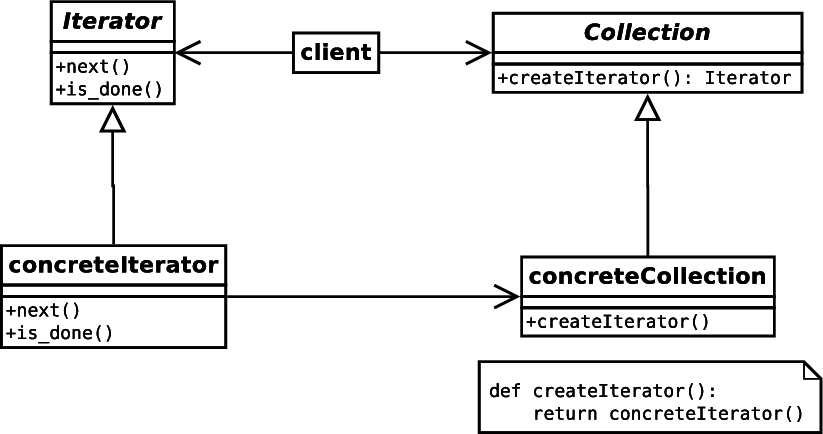
\includegraphics[width=0.75\textwidth]
    {../../diagrams/iterator_pattern.png}
  \caption{ Containers implement the Iterator pattern to allow sequential %
            access to items. }
  \label{fig:iterator_pattern}
\end{figure}


Python helps us create iterator objects by providing an Iterator protocol. In
Python, classes that define the \xfmethod{\_\_iter\_\_()} method can return an
iterator object.  The iterator object needs to define the \xfmethod{next()}
method, which provides the caller an element from the collection being iterated
over. The \xfclass{Container} class, \xfclass{ToolsList}, can act as an
iterator by defining the \xfmethod{\_\_iter\_\_()} and \xfmethod{next()}
methods. The only extra bit it needs to do is to keep track of the current
item, which it does through the \xfparameter{\_\_current\_item} variable, shown
in \Cref{lst:toolslist_iterator}.


\begin{xcode}{%
  language=Python,%
  label=lst:toolslist_iterator,%
  caption={The \xfclass{Container} class implements the Iterator pattern %
           to provide sequential access to items.}%
}
def Container(BasePageWidget):
    ...
    def __iter__(self):
        self.__current_item = 0
        return self

    def next(self):
        ...
        self.__current_item += 1

        if self.__current_item >= self__num_items:
            # reset our counter, stop iterating
            self.__current_item = 0
            raise StopIteration

        return self.get_item_by_position(self.__current_item)
\end{xcode}

The last task of a \xfclass{Container} class is to provide a way to search the
list for items that match some criteria. Two popular ways to access items from
the container are by position and by property.  The type of item returned by the
search methods is tied to the container returning it.  For example, a container
designed to represent a HUBzero support ticket list will return support ticket
list items and a container designed to represent a HUBzero group list will
return group list items.

To keep the \xfclass{Container} class generic, it implements the Factory Method
pattern, allowing subclasses to define which \xfclass{Item} class to
instantiate.

The Factory Method Pattern is used when we want to define an interface for
creating an object, but don't know which class to instantiate. Instead of
always instantiating the same class, we delegate the responsibility to a
subclass.

\begin{figure}[tbh]
  \centering
  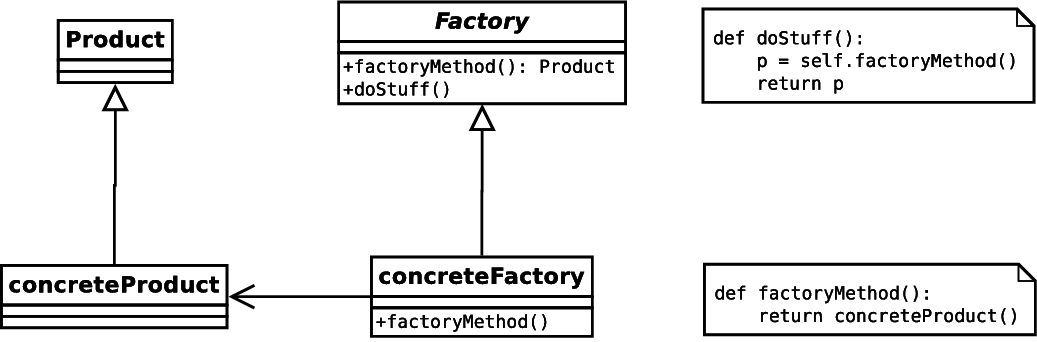
\includegraphics[width=0.75\textwidth]
    {../../diagrams/factory_method_pattern.png}
  \caption{ Containers use the Factory Method pattern to allow derived %
            classes determine the type of Item class to return from searches. }
  \label{fig:factory_method_pattern}
\end{figure}

In the case of the \xfclass{Container} class and the Tool Pipeline example, to
be able to return \xfclass{ToolsItem} objects from searches the
\xfclass{ToolsList} object must know how to create them. The \xfclass{Item}
class and parameters to create an object are saved by the derived container,
and then used by the search methods to instantiate the correct \xfclass{Item}
objects for the container.

\begin{xcode}{%
  language=Python,%
  label=lst:toolslist_constructor,%
  caption={The \xfclass{ToolsList} class manages which type of %
           \xfclass{Item} object to return from searches. In this %
           case \xfclass{ToolsItem} objects.}%
}
class Container(BasePageWidget):
    def __init__(self, owner, locatordict):
        self.item_class = None
        self.item_class_args = None

class ToolsList(Container):
    def __init__(self, owner, locatordict):
        ...
        self.item_class = ToolsItem
        self.item_class_args = [{...}]
\end{xcode}



The \xfclass{ToolsList} class provides two methods for searching through a list
of items.  The first method, \xfmethod{get\_item\_by\_position()}, allows
automation developers to search for an item in the list by position. For
example, developers can ask for the fifth item in the list.
\Cref{lst:toolslist_getitembyposition} shows an implementation of this method
that accepts a counting parameter, \xfparameter{item\_number}, representing the
n-th item in the list. The method uses the \xfclass{Container} object's
\xfclass{Item} class variable, \xfparameter{\_\_item\_class}, to construct the
\xfclass{Item} object for the n-th item in the list.
\xfparameter{\_\_item\_class} uses the \xfclass{Item} class parameters, stored
in \xfparameter{\_\_item\_class\_args}, and the method's
\xfparameter{item\_number} parameter to configure the new page object
representing the specific item.

\begin{xcode}{%
  language=Python,%
  label=lst:toolslist_getitembyposition,%
  caption={The Container class can retrieve Items by position}%
}
    def get_item_by_position(self,item_number):
        result = self.__item_class(
                  self.owner,
                  *self.__item_class_args,
                  item_number=item_number)
        result.detach_from_owner()
        return result
\end{xcode}

The second method, \xfmethod{get\_item\_by\_property()}, allows the developer to search
for the first item in the list that matches a property constraint.  The method
accepts two required parameters, the name of the property and the value it
should match.

\begin{xcode}{%
  language=Python,%
  label=lst:toolslist_getitembyproperty,%
  caption={The Container class can retrieve Items by property}%
}
    def get_item_by_property(self,prop,val):
        result = None

        # create a default item object, using the first item
        r = self.__item_class(self.owner,*self.__item_class_args,item_number=1)
        r.detach_from_owner()

        for item_number in xrange(1,len(items)+1):

            # update the default item object to point to the current item
            r.update_item_number(item_number)

            # check if our current item matches the property constraint
            if r.value()[prop] == val:
              result = r
              break

        # if no items matched, clean up our default item object
        if result is None:
          del r

        return result
\end{xcode}

The \xfmethod{get\_item\_by\_property()} method also uses the
\xfparameter{\_\_item\_class} variable, representing the \xfclass{Item} class,
to construct a new page object that represents a single item in the list.
Similar to the \xfmethod{get\_item\_by\_position()} method, the
\xfmethod{get\_item\_by\_property()} method passes the
\xfparameter{\_\_item\_class}'s constructor a list of arguments to configure
the new page object, including a dictionary of locator templates.

The \xfmethod{get\_item\_by\_property()} method uses an \xfclass{Item} object
to iterate over the items in the list, searching for the first item that
satisfies the property constraint. It takes advantage of the \xfclass{Item}
object's \xfmethod{update\_item\_number()} method and template locators to
update the locators of the object without instantiating a new page object for
each item it encounters in the list. In
\Cref{lst:toolslist_getitembyproperty}, you can see the \xfclass{Item} object
being updated inside of the for loop in line 11, and the comparison between the
item's property and the requested value in line 14.



The ItemList pattern focuses on the interactions of two classes, the
\xfclass{Container} class and the \xfclass{Item} class. In the Tool Pipeline
table example the \xfclass{Container} class, \xfclass{ToolsList}, was
responsible for all of the services provided by the table that were not related
to a specific item or item in the table. The \xfclass{Item} class,
\xfclass{ToolsItem} was responsible for services associated with a specific
item or item in the table.  This separation of services, along with the use of
web element locator templates, allowed the \xfclass{Container} class to
dynamically create page objects for specific items in the table and update the
item being referenced without needing to destroy and create a new object.



\subsection{IframeWrap Pattern}
\label{ssec:iframewrap_pattern}

%
% Used to quickly navigate through layers of iframes to interact with web page
% widgets.

% \subsection{Pattern Name and Classification:}
%
%   IframeWrap Pattern
%   Purpose: Structural - we are defining a good way to dynamically create
%                         a page object to describe and access a specific
%                         item in a list of items.
%   Scope: Object
%

Iframes are another area where using the wrong design can make page objects
difficult to build and inefficient to use and maintain. When hub users upload
resources to a HUBzero website, they are asked to respond to several questions
on a web form, one of which involves describing the resource they are
contributing.  In previous incarnations, the resource contribution form's
description field was a simple HTML <textarea> element. The field handled both
plain text descriptions, but also allowed users to enter a wiki-like markup
language that produced rich text descriptions.  Building a page object with a
<textarea> is pretty rudimentary, and in HUBcheck is represented by the
\xfclass{TextArea} class.


\begin{figure}[tbh]
  \centering
  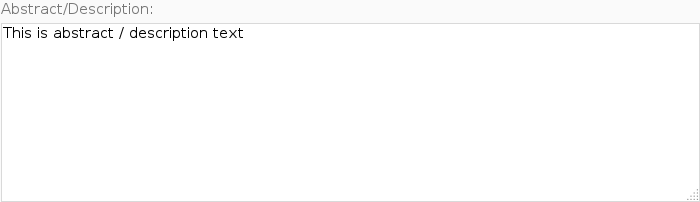
\includegraphics[width=0.75\textwidth]
    {../../images/hubzero_new_resource_compose_step_abstract_textarea.png}
  \caption{HTML <textarea> based editor. }
  \label{fig:html_textarea_editor_widget}
\end{figure}

\begin{xcode}{%
  language=HTML,%
  label=lst:html_textarea_editor_code,%
  caption={HTML of the textarea based editor.}%
}
<label for="field-fulltxt">
    Abstract/Description:
    <textarea id="field-fulltxt">This is abstract / description text</textarea>
</label>
\end{xcode}

Around the release of version 1.2.0 of the HUBzero software, the web developers
started incorporating a new editor for the description field. Shown in
\Cref{fig:html_iframe_editor_widget}, the new editor incorporated better
controls for handling rich text.  Instead of writing out the wiki syntax to
make words bold, for example, the hub user would press the bold button in the
editor and type the text they wanted to be bold.  This was a great step forward
for usability. The updated editor meant an update was needed for the page
objects that interacted with the previously available <textarea> based editor.
Such a drastic widget change like this usually results in a new page object
being created.



\begin{figure}[tbh]
  \centering
  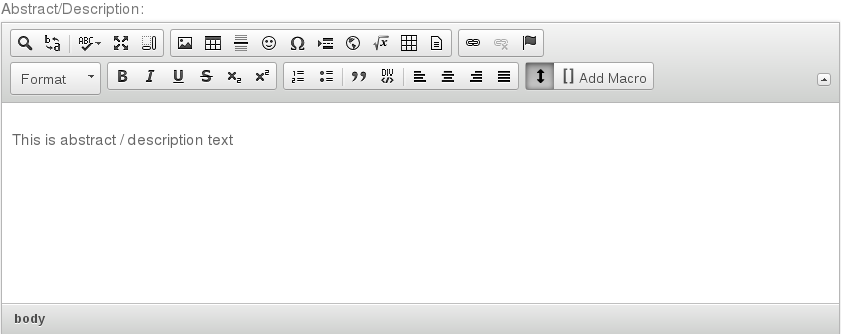
\includegraphics[width=0.75\textwidth]
    {../../images/mygeohub_new_resource_compose_step_abstract_texteditor.png}
  \caption{HTML iframe based editor.}
  \label{fig:html_iframe_editor_widget}
\end{figure}

\begin{xcode}{%
  language=HTML,%
  label=lst:html_iframe_editor_code,%
  caption={HTML of the iframe based editor, where writing to the %
           <body> tag is just like writing to the %
           <textarea> tag after the automation script %
           enters the iframe.} %
}
<iframe class="cke_wysiwg_frame">
    <html>
        <body class="ckeditor-body">
            <p>This is abstract / description text </p>
        </body>
    </html>
</iframe>
\end{xcode}

Investigating the new web page, one could see that the previous <textarea>
element was replaced with an iframe and embedded web page. Playing around with
the iframe element revealed that once the automation script entered the iframe,
writing text to the <body> element was just like writing text to the <textarea>
element.  This raised the question: \begin{quote}\textit{Do I need to write a
new page object class for an element embedded in an iframe, if a class for that
element already exists and works with the exception of entering and exiting the
iframe?}\end{quote}


\begin{figure}[tbh]
  \centering
  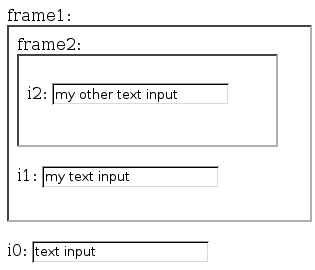
\includegraphics[width=0.50\textwidth]
    {../../images/iframewrap_inputs_example_base.png}
  \caption{Text input fields embedded in different levels of iframes.}
  \label{fig:iframewrap_inputs_example_base}
\end{figure}


Before approaching this question, let's first investigate how iframes work.
\Cref{fig:iframewrap_inputs_example_base} shows an example web page with
some input fields embedded in different levels of iframes.

\begin{figure}[tbh]
  \centering
  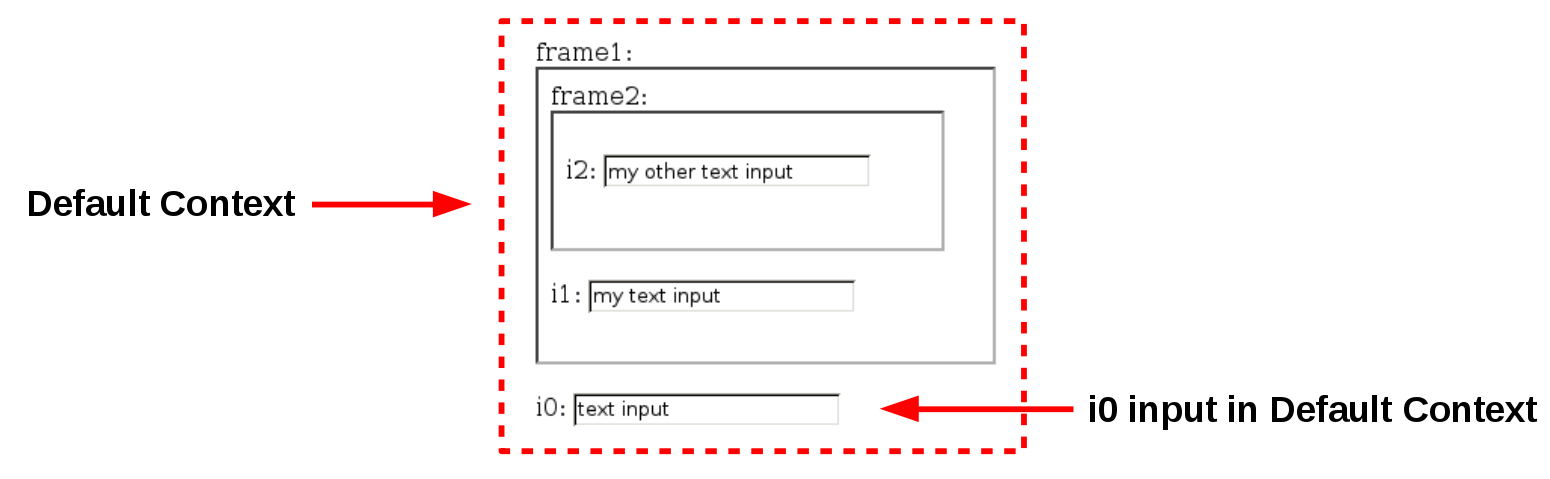
\includegraphics[width=0.75\textwidth]
    {../../images/iframewrap_inputs_example_frame_0.png}
  \caption{Text input i0 exists in the default context.}
  \label{fig:iframewrap_inputs_example_frame_0}
\end{figure}

\begin{xcode}{%
  language=HTML,%
  label=lst:html_iframe_example_default_context,%
  caption={In the default context, iframe frame1 references inner\_page.html.}%
}
<html>
    <body>
        <label for="frame1">frame1: </label>
        <iframe id="frame1" src="inner_page.html"></iframe>
        <br/><br/>
        <label for="i0">i0: </label>
        <input type="text" id="i0" value="text input"></input>
    </body>
</html>
\end{xcode}


The first input field, i0, is located in the default context. This is the level
of the web page we generally work in when iframes are not involved.  Along with
the input field i0, this web page also has an iframe, frame1.  In the HTML,
iframes hold the location of another web page to be embedded in the frame. In
this example, frame1 is going to load up the web page inner\_page.html.


\begin{figure}[tbh]
  \centering
  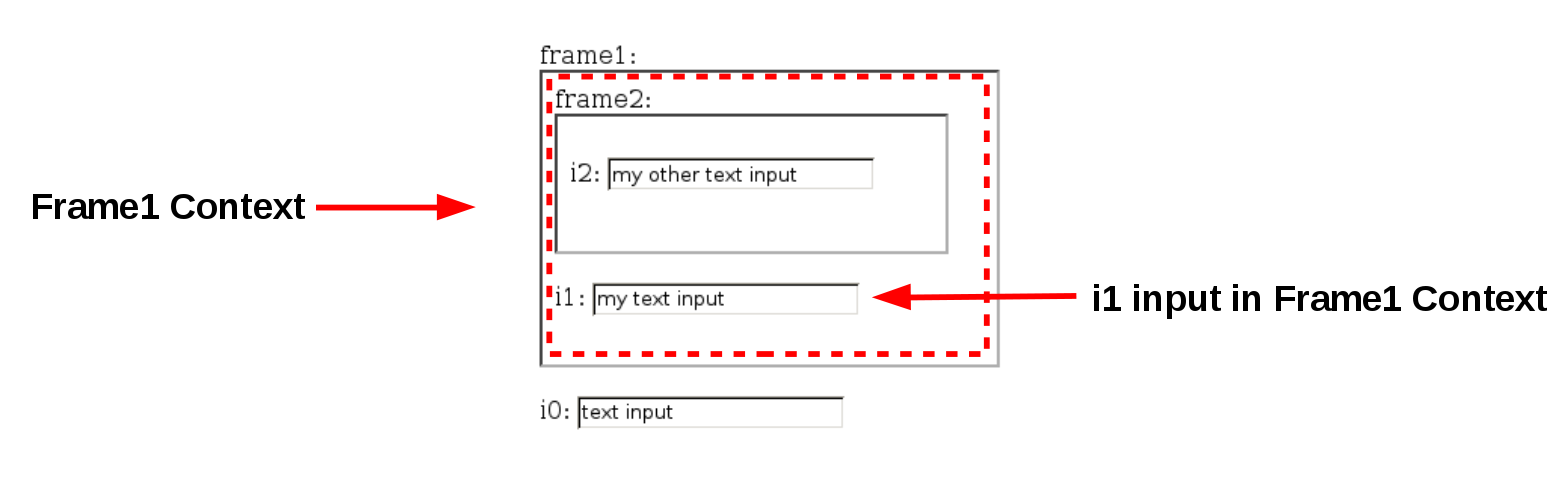
\includegraphics[width=0.75\textwidth]
    {../../images/iframewrap_inputs_example_frame_1.png}
  \caption{Text input i1 exists in the frame1 context.}
  \label{fig:iframewrap_inputs_example_frame_1}
\end{figure}

\begin{xcode}{%
  language=HTML,%
  label=lst:html_iframe_example_frame1_context,%
  caption={inner\_page.html - frame2 references another\_page.html.}%
}
<html>
    <body>
        <label for="frame2">frame2: </label>
        <iframe id="frame2" src="another_page.html"></iframe>
        <br/><br/>
        <label for="i1">i1: </label>
        <input type="text" id="i1" value="my text input"></input>
    </body>
</html>
\end{xcode}

\Cref{fig:iframewrap_inputs_example_frame_1} and
\Cref{lst:html_iframe_example_frame1_context} show the HTML for
inner\_page.html.  It makes up what is referred to as the Frame1 Context. The
Frame1 context has an input field i1, and another iframe, frame2.  Again, the
iframe frame2 holds the location of a web page, and in this case it points to
another\_page.html.


\begin{figure}[tbh]
  \centering
  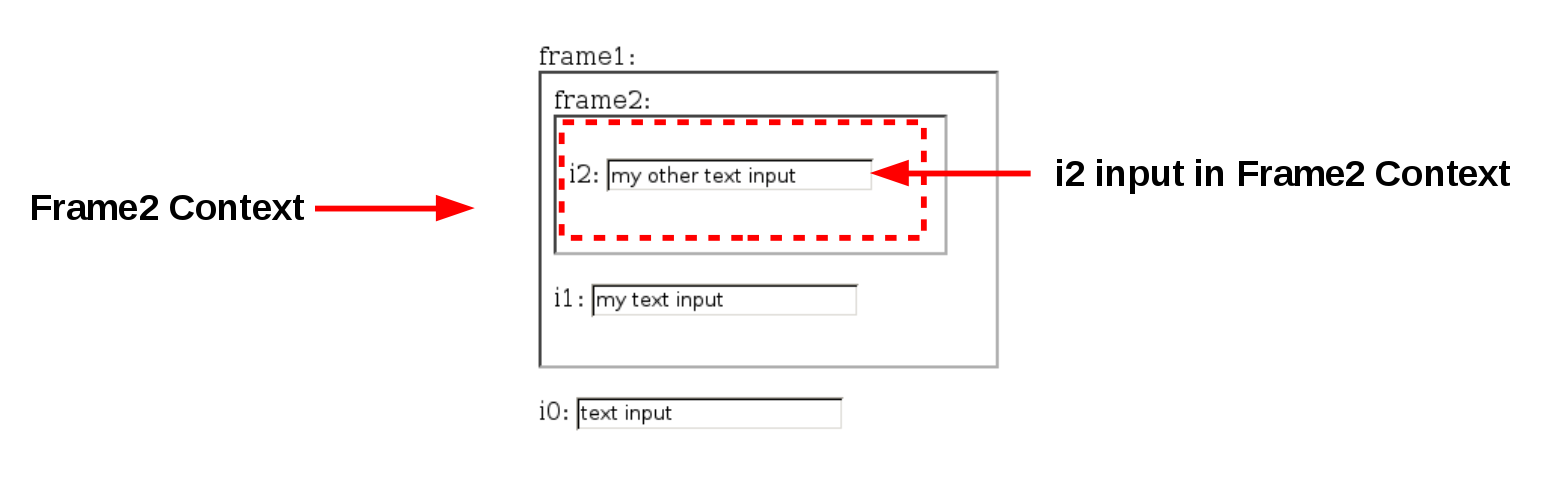
\includegraphics[width=0.75\textwidth]
    {../../images/iframewrap_inputs_example_frame_2.png}
  \caption{Text input i2 exists in the frame2 context.}
  \label{fig:iframewrap_inputs_example_frame_2}
\end{figure}

\begin{xcode}{%
  language=HTML,%
  label=lst:html_iframe_example_frame2_context,%
  caption={another\_page.html - in frame2 context, only input i2 exists.}%
}
<html>
    <body>
        <label for="i2">i2: </label>
        <input type="text" id="i2" value="my other text input"></input>
    </body>
</html>
\end{xcode}


\Cref{lst:html_iframe_example_frame2_context} shows the HTML for the
file another\_page.html that makes up the Frame2 Context. It contains an input
field i2 that resides within the Frame2 context.


\begin{xcode}{%
  language=Python,%
  label=lst:text_input_field_i0_class,%
  caption={Page object class for i0 text input field.}%
}
class Text(BasePageWidget):
    ...
    # setter
    def value(self, text):
        e = self.find_element(self.locator)
        e.clear()
        e.send_keys(text)
    ...
\end{xcode}

A page object for the i0 input field that resides in the Default Context
would probably include a getter method to retrieve the value of the input, a
setter method to set the value of the input, and maybe an append method to
assist with appending text to whatever was already in the field.  Since the i0
field resides in the default context, there is no need to do anything special;
the methods will find the i0 input element in the HTML DOM, and perform actions
on it.

\begin{xcode}{%
  language=Python,%
  label=lst:text_input_field_i1_class,%
  caption={Page object class for i1 text <input> field.}%
}
class Text1Frame(BasePageWidget):
    ...
    # setter
    def value(self, text):
        frame = self.find_element('#frame1')
        self._browser.switch_to_frame(frame)
        e = self.find_element(self.locator)
        e.clear()
        e.send_keys(text)
        self._browser.switch_to_default_content()
    ...
\end{xcode}

Building a page object for the i1 input field involves a little more work.
The page object is almost the same as the one for the i0 input field, but
because i1 is located inside of the Frame1 context the web browser needs to be
instructed to traverse the frame1 iframe before performing any getter, setter,
or append actions.  So inside each of the page object's methods a few lines of
code need to be added for entering and exiting the iframe. After the web
browser has entered the Frame1 context it can search for the element in the
HTML DOM and perform actions on the element.  In
\Cref{lst:text_input_field_i1_class}, the extra code for entering and exiting
the Frame1 context shows up in lines 5-6 and line 10.  Lines 7-9 make up the
core action of the widget and are the same as what is found in the page object
for text input i0, in \Cref{lst:text_input_field_i0_class}.


\begin{xcode}{%
  language=Python,%
  label=lst:text_input_field_i2_class,%
  caption={Page object class for i2 text input field.}%
}
class Text2Frame(BasePageWidget):
    ...
    # setter
    def value(self, text):
        frame1 = self.find_element('#frame1')
        self._browser.switch_to_frame(frame1)
        frame2 = self.find_element('#frame2')
        self._browser.switch_to_frame(frame2)
        e = self.find_element(self.locator)
        e.clear()
        e.send_keys(text)
        self._browser.switch_to_default_content()
    ...
\end{xcode}

Building a page object for the i2 input field adds another layer of iframe
context traversal.  Remember, i2 is located inside of the Frame2 context, which
is located inside of the Frame1 context. The methods for the i2 page object
have the same core actions as those of the i0 and i1 page objects, but include
code to traverse two iframe contexts. This can be seen in
\Cref{lst:text_input_field_i2_class}, where the setter method first moves from
the Default context to the Frame1 context in lines 5-6, then moves from the
Frame1 to the Frame2 context in lines 7-8. The setter method next performs the
method's core action in lines 9-11 and finally returns back to the default
context in line 12.


To review, building page objects for the i0, i1 and i2 input fields involves
tracking the current frame level and possibly traversing frame levels to be in
the correct context for interacting with an element.  In the example from
\Cref{fig:iframewrap_inputs_example_base}, all of the page objects
started off with the same code, but for input i1, additional lines were added
to account for entering and exiting the Frame1 context.  Similarly, for input
i2, additional lines of code were added to account for entering and exiting the
Frame1 and Frame2 contexts.  But the question remains: \begin{quote}\textit{Is there a way
to handle the entering and exiting of iframes outside of the page object so we
can reuse our original page object that represents a Text <input> field on a
web page?}\end{quote}

In essence, a solution would provide a way to write the core methods of a page
object once and if the page object was found inside of an iframe, the methods
could be wrapped with code to enter and exit the iframe. If the page object was
found inside of two, or three, or more iframes, the methods would just keep
getting wrapped with code to enter and exit iframe contexts.


\begin{figure}[tbh]
  \centering
  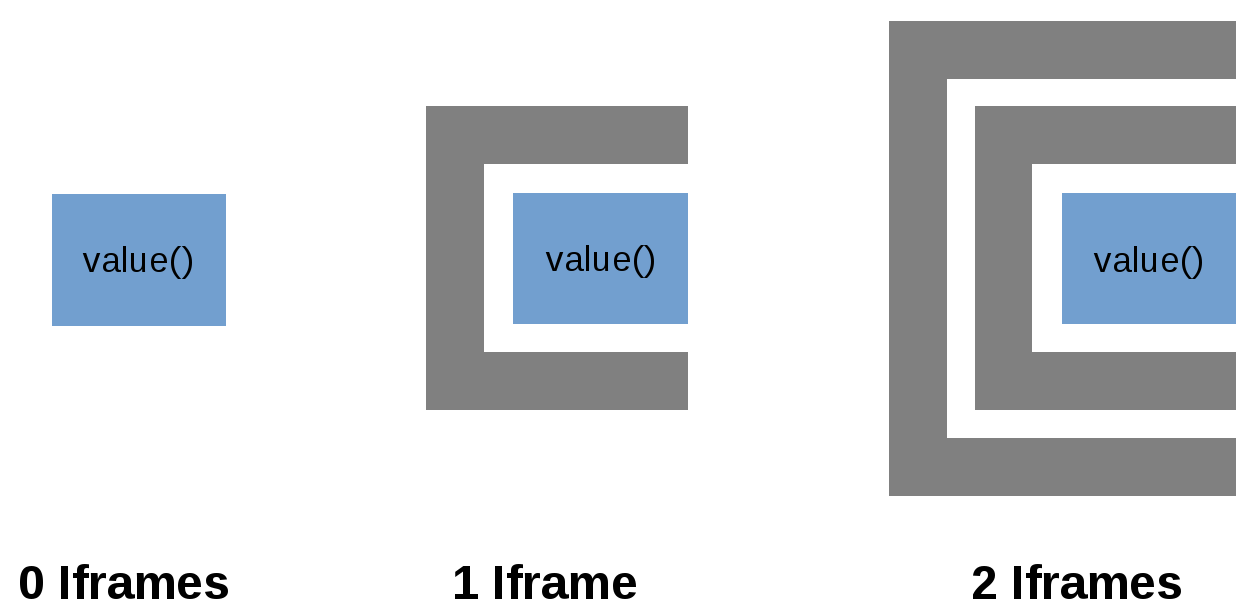
\includegraphics[width=0.75\textwidth]
    {../../images/iframewrap_pattern_multiple_frames.png}
  \caption{IframeWrap pattern wraps the core of methods with code to %
           traverse iframe contexts.}
  \label{fig:iframewrap_pattern_multiple_frames}
\end{figure}


This is the idea behind the IframeWrap pattern. It uses the Decorator pattern
to \textit{decorate} or wrap the attributes of a page object with code to enter
an iframe context, call the original page object method, and then exit the
iframe context. It supports both page objects from the default context as well
as previously wrapped page objects.


\begin{figure}[tbh]
  \centering
  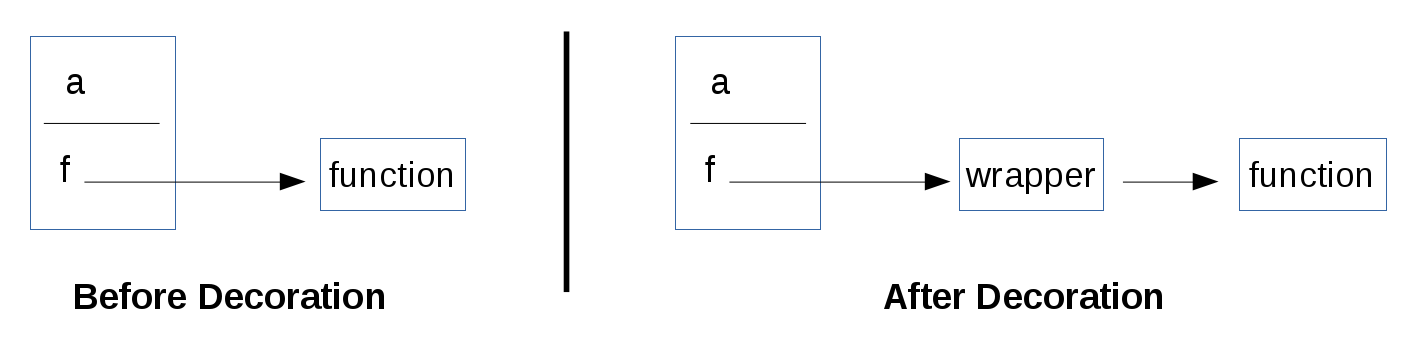
\includegraphics[width=0.75\textwidth]
    {../../images/decorator_pattern_before_after.png}
  \caption{Decorator pattern}
  \label{fig:decorator_pattern}
\end{figure}


The purpose of the Decorator pattern is to extend functionality of an object
without necessarily changing the interface. It is most often used when a
specific object needs to be changed at runtime without affecting other objects
of the class.  It does this by wrapping the original functionality of the
object's attributes with code to do extra work.

Consider the example object \xfobject{a} shown in \Cref{fig:decorator_pattern},
which is an instance of the class \xfclass{A}, with a method \xfmethod{f}.
Additional responsibilities can be added to \xfobject{a}'s method \xfmethod{f}
by first pointing \xfparameter{a.f} to a wrapper method and then directing the
wrapper method to perform the extra work and call the method that
\xfparameter{a.f} used to point to.

\begin{figure}[tbh]
  \centering
  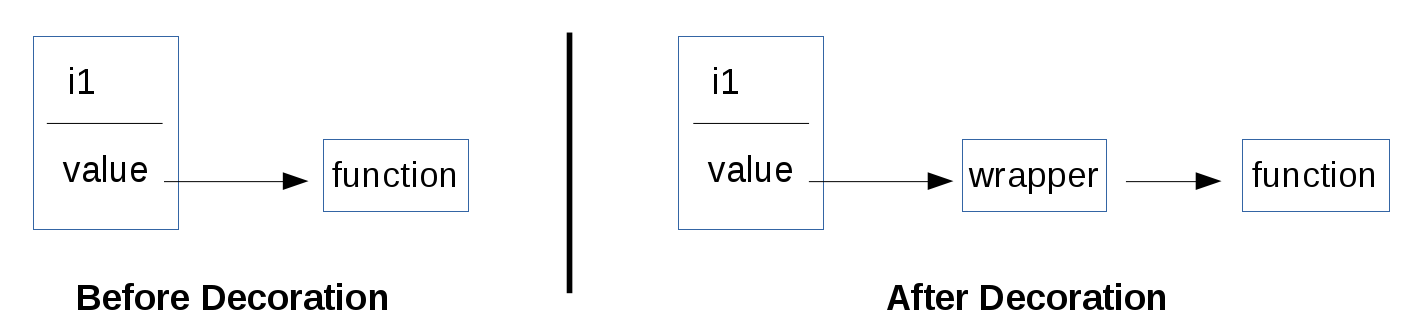
\includegraphics[width=0.75\textwidth]
    {../../images/decorator_pattern_applied_to_i1.png}
  \caption{Decorator pattern applied to text input field i1 in Frame1 context}
  \label{fig:decorator_pattern_i1}
\end{figure}


The same idea can be applied to the \xfclass{Text} page object, from
\Cref{lst:text_input_field_i0_class}, to create a page object for the i1 input
in the Frame1 context. The page object's \xfmethod{value()} method performs the
core actions for setting or getting the value of the underlying HTML element.
In Python, \xfmethod{value()} is an attribute that points to a function object,
which can be decorated to add the enter and exit iframe commands.  After
decorating the function object, the value attribute will point to a wrapper
function that enters the correct iframe context, calls the original function
object, and returns back to the default context.


\begin{xcode}{%
  language=Python,%
  label=lst:iframewrap_example_po,%
  caption={Page object class for web page with multiple text input field %
           embedded in frames.}%
}
class FramedInputs(BasePageObject):
    def __init__(self):
        self.i0 = Text('#i0')
        self.i1 = IframeWrap( Text('#i1'), ['#frame1'] )
        self.i2 = IframeWrap( Text('#i2'), ['#frame2', '#frame1'] )
\end{xcode}

A page object class that represents the web page shown in
\Cref{fig:iframewrap_inputs_example_base} can be built by instantiating and
decorating the \xfclass{Text} class from \Cref{lst:text_input_field_i0_class}.
In \Cref{lst:iframewrap_example_po}, the variable self.i0 instantiates a
\xfclass{Text} object to represent the text input field in the default context.
The variables self.i1 and self.i2 also instantiate \xfclass{Text} objects, but
immediately passes them to the \xfmethod{IframeWrap()} function. The
\xfmethod{IframeWrap()} function accepts a page object and a list of locators
for frames that must be traversed to access the element represented by the page
object. For example, the i1 text input field resides within a frame with a
locator \xflocator{\#frame1}, so the \xfmethod{IframeWrap()} function is sent
the single element list \xfinlinecode{['\#frame1']}.  Similarly, the i2 text
input field resides in a frame with a locator \xflocator{\#frame2}, which
itself resides in a frame with a locator \xflocator{\#frame1}, so the
\xfmethod{IframeWrap()} function is sent a two element list containing both
locators.


\begin{xcode}{%
  language=Python,%
  label=lst:iframetracker_class,%
  caption={\xfclass{IframeTracker} objects manage wrapping object methods %
           and attributes}%
}
class IframeTracker(object):
    ...
    def wrap_callable_attributes(self,o):
        for attr, item in o.__class__.__dict__.items():
            if callable(item):
                item = getattr(o,attr)
                setattr(o,attr,self.wrap_attribute(item))

    def wrap_attribute(self,item):
        def wrapper(*args, **kwargs):
            ...
            switched = self._switch_to_iframe_context(final_framelevel)
            result = item(*args, **kwargs)
            self._switch_to_iframe_context(initial_framelevel)
            return result
        return wrapper
\end{xcode}



Internally, the \xfmethod{IframeWrap()} function creates an
\xfclass{IframeTracker} object and associates it with the page object that is
to be decorated. The \xfclass{IframeTracker} object is responsible for tracking
frame levels and wrapping the object's attributes.  The most interesting part
of the \xfclass{IframeTracker} object is when the page object gets decorated,
which is shown in \Cref{lst:iframetracker_class}.  First the
\xfmethod{IframeWrap()} method calls the
\xfmethod{wrap\_callable\_attributes()} method, which identifies callable
attributes from the object, including methods. Within the page object, the
callable attribute is replaced with a call to the \xfmethod{wrapper()} method,
which is a closure that stores the function object it replaces.  Just as shown
in \Cref{fig:decorator_pattern}, the \xfmethod{wrapper()} method takes
care of entering the correct frame context, calling the original method it
replaces that performs the core actions, and returning back to the original
frame context.


\begin{xcode}{%
  language=Python,%
  label=lst:iframewrapd_po_use,%
  caption={IframeWrap'd page objects work just like non-wrapped page objects.}%
}
class FramedInputs(BasePageObject):
    def __init__(self):
        self.i0 = Text('#i0')
        self.i1 = IframeWrap( Text('#i1'), ['#frame1'] )
        self.i2 = IframeWrap( Text('#i2'), ['#frame2', '#frame1'] )


po = FramedInputs()

# print out the current text in the widgets
print "i0.value = %s" % (po.i0.value)
print "i1.value = %s" % (po.i1.value)
print "i2.value = %s" % (po.i2.value)

# update the text in the widgets
po.i0.value = 'i0 text'
po.i1.value = 'new i1 text'
po.i2.value = 'new i2 text too'
\end{xcode}


With the page object attribute wrapping process complete, the newly
IframeWrap'd page object is ready for use. Inside of automation scripts, the
decorated page objects work just like the non-decorated page objects. The
automation developer doesn't need to do anything special to access or interact
with the wrapped page objects. In \Cref{lst:iframewrapd_po_use}, the variables
i0, i1, and i2 are all accessed from the page object po in the same way.  The
responsibility for managing the frame traversal has been embedded within the
page object. The difference between text input field page objects is only
exposed in how the page objects are instantiated.

When implementing the IframeWrap pattern in Python there are a few gotchas. Not
all page object attributes need to be wrapped. Some attributes do not try to
interact with the web element the page object represents. Keeping a list of
these attributes is handy so the wrapping of these attributes can be skipped.
Additionally wrapping Python object properties can be tricky because properties
are a part of the class, not the object. It requires creating a new class
object from the page object's class, decorating the properties of the new class
object, and associating the page object with the new class.



\section{Summary of Page Object Based Design Patterns}
\label{sec:summary_page_object_design_pattern}

The Page Object design pattern provides developers with an object-oriented way
to think about dissecting web pages. Its framework for creating reusable pieces
of code to represent parts of web pages can simplify the process of building
robust web automation software, but sometimes taking a naive approach can lead
to an inefficient page object design. In this chapter, we saw three situations
where implementing a naive page object design could lead to inefficient
programs. Instead, more robust designs were offered as solutions which helped
increase code reuse.

The first situation involved the frequent situation of building page objects
for web forms.  Due to similarities in the design and goals of web forms, we were
able to reduce their use to answering questions, filling the answers into fields
on the web page, and pressing the submit or cancel button. This generalization of
goals allowed us to recognize that with the exception of the specific fields
that needed to be populated, a large portion of building page objects for web
forms could be abstracted into a generic \xfclass{Form} superclass. Fields
could then be specified in a derived subclass.

In the second case we investigated building page objects for lists of items on
a web page where there is no a priori knowledge of the number of items
displayed.  The ItemList Pattern encourages users to build a single page object
to represent an item in a list, and update which item in the list the page
object points to instead of trying to build a separate class for each item in
the list.

Lastly, we considered building page objects for web page elements that exist in
different iframe levels. While it may be tempting to manually create a new page
object class for an element that exists in an iframe, this approach discourages
code reuse. Instead, the IframeWrap pattern decorates a page object's
attributes with additional code to enter and exit the proper iframe context
without changing the original object's interface.


% building tests and tools with hubcheck libraries
% how does selenium work
% description of hubcheck libraries built on top of selenium
% example uses of selenium based hubcheck libraries
% how does expect work
% hubcheck libraries built on top of expect
% example uses of expect based hubcheck libraries
% how to use the libraries to build tests
% how to use the libraries to build tools
%\include{selenium1}
%\include{pageobjects}
%\include{shell_automation}

% case studies of using hubcheck to identify errors
% case study 1: testing web components
% case study 2: testing tool session containers
% case study 3: finding bad links
% case study 4: Rappture nightly build and test
% case study 5: BD testing?
% \include{casestudy_contribtool}
% \include{casestudy_bad_links}

% Summary and/or conclusions are optional but often used.
% The summary and/or conclusions often are the last
% major division(s) of the text.
% Reference: TM 32.
% CHANGE NEXT LINE?
%\include{summary}
%
%  solutions.tex  2014-12-12  Derrick Kearney created solutions.tex
%
%  Describe how hubcheck is being used to monitor that components of hubs
%  continue to work through software upgrades.
%

% outline:
%
% 1) hubcheck has been deployed to run nightly and weekly tests on hubs
%    the success of hubcheck at alerting us to problems varies.
% 2) introduced 3 new design patterns for building selenium page objects.
% 3) created python modules for interacting with hub tool session containers
%    through SSH/SFTP and some parts of the hub website through Selenium Webdriver.
% 4) can verify correct setup of tool session containers in 1 hour, running 150 tests.
%
% -------------
%

%
% -------------
%
% Summary of results from weekly hubcheck runs:
%
% 1) turbulent hubs
%   -> ccehub
%     * website dashboard web page
%       members_dashboard_my_session_item.test_quick_launch
%       members_dashboard_my_session_storage.test_storage_meter
%     * container packages
%       container_packages.test_wheezy_packages
%     * debian 7 tool session container config
%       container_use_config.test_apps_share64_environ_rappture_link
%       container_use_config.test_apps_share64_environ_rappture_dev_link
%       container_use_config.test_apps_environ_setup_sh_does_not_exist
%       container_icewm_config.test_userconfig_icewm_toolbar
%       container_icewm_config.test_userconfig_icewm_theme
%       container_icewm_config.test_userconfig_icewm_preferences
%       container_icewm_config.test_userconfig_icewm_menu
%       container_icewm_config.test_userconfig_icewm_keys
%       container_config.test_paths_startxvnc
%       container_config.test_paths_pixelflip
%       container_config.test_paths_mergeauth
%       container_config.test_paths_clientaction
%
% 2) new hubs being brought online
%   -> mygeohub
%     * tty problem
%       TestRegisteredUser2.test_tty_recycle
%     * submit, pegasus missing
%       TestContainerSubmitParameterExamples.test_submit_parameter_error_code
%       TestContainerSubmitParameterExamples.test_submit_parameter_glob_file_search
%       TestContainerSubmitParameterExamples.test_submit_parameter_substitute_in_command_arguments
%       TestContainerSubmitParameterExamples.test_submit_change_separator
%       TestContainerSubmitParameterExamples.test_submit_read_csv_params_load_extras_from_file
%       TestContainerSubmitParameterExamples.test_submit_read_csv_params_load_extras_from_args
%       TestContainerSubmitParameterExamples.test_submit_read_params_from_csv_file
%       TestContainerSubmitParameterExamples.test_submit_read_params_file_load_extra_params
%       TestContainerSubmitParameterExamples.test_submit_read_parameters_from_file
%       TestContainerSubmitParameterExamples.test_submit_multiple_parameter_substitution
%       TestContainerSubmitParameterExamples.test_submit_single_parameter_substitution
%     * debian 7 container config
%       container_use_config.test_apps_share_environ_is_directory
%       container_use_config.test_apps_share64_environ_is_directory
%     * container packages
%       container_packages.test_wheezy_packages
%     * website tool session webpage (is there a ticket for this, mygeohub_weekly_20140519024000.log)
%       members_dashboard_my_session_item.test_resume_click
%
% 3) old hubs being upgraded
%   -> pharmahub
%     * submit not working, pegasus missing
%       container_submit_parameter_examples.test_submit_read_params_from_csv_file
%       container_submit_parameter_examples.test_submit_read_params_file_load_extra_params
%       container_submit_parameter_examples.test_submit_read_parameters_from_file
%       container_submit_parameter_examples.test_submit_read_csv_params_load_extras_from_file
%       container_submit_parameter_examples.test_submit_read_csv_params_load_extras_from_args
%       container_submit_parameter_examples.test_submit_parameter_substitute_in_command_arguments
%       container_submit_parameter_examples.test_submit_parameter_glob_file_search
%       container_submit_parameter_examples.test_submit_parameter_error_code
%       container_submit_parameter_examples.test_submit_multiple_parameter_substitution
%       container_submit_parameter_examples.test_submit_change_separator
%     * missing packages:
%       container_packages.test_wheezy_packages
%     * debian 7 tool session container configuration
%       container_use_config.test_apps_share64_environ_rappture_link
%       container_use_config.test_apps_share64_environ_rappture_dev_link
%       container_use_config.test_apps_environ_setup_sh_does_not_exist
%       container_use_config.test_apps_environ_setup_csh_does_not_exist
%       container_config.test_paths_startxvnc
%       container_config.test_paths_pixelflip
%       container_config.test_paths_mergeauth
%       container_config.test_paths_importfile
%       container_config.test_paths_filexfer
%       container_config.test_paths_exportfile
%       container_config.test_paths_clientaction
%
% 4) bugs discovered by hubcheck
%   -> molecularhub, habricentral
%     * side effect of https://hubzero.org/support/ticket/5254 (molecularhub)
%                      https://hubzero.org/support/ticket/5255 (habricentral)
%       parameter_passing_invoke_app_tests.test_1_command_no_templates_no_parameters_file
%       parameter_passing_invoke_app_tests.test_1_command_no_templates_with_parameters_file
%       parameter_passing_invoke_app_tests.test_1_template_0_default_run_template_1
%       parameter_passing_invoke_app_tests.test_1_template_1_default_run_default
%       parameter_passing_invoke_app_tests.test_1_template_1_default_run_template
%     * side effect of https://hubzero.org/support/ticket/5317
%       parameter_passing_url_tests.test_launch_tool_blacklisted_path_1
%       parameter_passing_url_tests.test_launch_tool_invalid_path_4
%     * parameter passing not installed on hub?
%       parameter_passing_url_tests.test_launch_tool_file_format_1
%       parameter_passing_url_tests.test_launch_tool_file_format_2
%       parameter_passing_url_tests.test_launch_tool_file_format_3
%       parameter_passing_url_tests.test_launch_tool_file_format_4
%       parameter_passing_url_tests.test_launch_tool_file_format_5
%       parameter_passing_url_tests.test_launch_tool_file_format_6
%       parameter_passing_url_tests.test_launch_tool_home_expansion_1
%       parameter_passing_url_tests.test_launch_tool_named_file_1
%       parameter_passing_url_tests.test_launch_tool_named_file_2
%       parameter_passing_url_tests.test_launch_tool_whitelisted_path_3
%   -> purr
%     * side effect of https://hubzero.org/support/ticket/5284
%       override causing php to fail before rendering
%       the parameter passing tests may have still passed if we didn't use
%       the tool session web page to see if the session started and to
%       find the session id, but the TestToolSessionApp and TestToolSessionShare
%       tests would still have failed.
%       parameter_passing_invoke_app_tests.test_1_template_0_default_run_template_1
%       parameter_passing_invoke_app_tests.test_1_template_1_default_run_default
%       parameter_passing_invoke_app_tests.test_1_template_1_default_run_template
%       parameter_passing_url_tests.test_launch_tool_file_format_1
%       parameter_passing_url_tests.test_launch_tool_file_format_2
%       parameter_passing_url_tests.test_launch_tool_file_format_3
%       parameter_passing_url_tests.test_launch_tool_file_format_4
%       parameter_passing_url_tests.test_launch_tool_file_format_5
%       parameter_passing_url_tests.test_launch_tool_file_format_6
%       parameter_passing_url_tests.test_launch_tool_home_expansion_1
%       parameter_passing_url_tests.test_launch_tool_named_file_1
%       parameter_passing_url_tests.test_launch_tool_named_file_2
%       parameter_passing_url_tests.test_launch_tool_no_parameters_file
%       parameter_passing_url_tests.test_launch_tool_whitelisted_path_3
%       TestToolSessionApp.test_storage_meter
%       TestToolSessionShare.test_share_session_with_1
%       TestToolSessionShare.test_share_session_with_2
%       TestToolSessionShare.test_share_session_with_3
%       TestToolSessionShare.test_share_session_with_6
%       TestToolSessionShare.test_share_session_with_7
%       TestToolSessionShare.test_share_session_with_8
%       TestToolSessionShare.test_disconnect_1
%     * HAR 500 error? trouble launching tool session container
%       parameter_passing_invoke_app_tests.test_1_command_no_templates_no_parameters_file
%       parameter_passing_invoke_app_tests.test_1_command_no_templates_with_parameters_file
%   -> drinet - no parampassing tests, all issues died when hub was shut down:
%       https://hubzero.org/support/ticket/5328


%In 2013 we started running automated tests on a regular basis on the hubs. In
%February 2014, we deployed a Jenkins server to help manage the automated tests
%and make the test results more accessable to the group. Between February 2014
%and November 2014, we were able to track the results of automated tests. Over
%this time period we have been able to use hubcheck to monitor hubs for bugs as
%they receive website and tool session container upgrades. 


\chapter{HUBCHECK AS A SOLUTION}
\label{chap:solution}

In February of 2014, the HUBzero team deployed a Jenkins
\cite{Jenkins:2015:Online} continuous integration server to help manage
automated tests being run by HUBcheck and to make test results more accessible
to members of the team. Since then, automated test results have been tracked
for runs against the weekly and nightly test suites, two of the most frequently run test
suites offered by HUBcheck. Through the use of the weekly and nightly test
suites, the HUBzero team was able to track the health of hubs and resolve
differences in their setup as they receive website and tool session container
upgrades.

The HUBzero team has tracked the long term results of two of HUBcheck's test
suites. The nightly suite contains 11 test cases that focus on tool session
container access and job submission through the \xfprogramname{submit} command. The
weekly suite contains over 150 test cases and dives deeper into the setup and
workings of the tool session container, including some of the most tedious
tasks to check, which involve interaction between the user's website and tool
session container. As their names suggest, the nightly and weekly suites run on
a nightly and weekly basis respectively.

The health of a hub can be categorized as either \textit{Turbulent},
\textit{Upgraded}, or \textit{New}. Below, we look at each categorization and
use the HUBcheck's weekly and nightly test suites to help identify
opportunities for improvement in the roll out, maintenance, and upgrade of hubs.


\section{Turbulent Hubs}
\label{sec:solution_turbulent}
% explain the meaning of the category
% give an idea of how to identify a hub that fits into this category from the plots
% analyze the experience of one hub that is the representative for this category
% tell how hubs are moved out of this category to a better category.
% give recommendations on how to keep hubs from falling into this category.
%

% between 20140201 and 20150201, 73 new tickets were created on the system.  2
% support tickets on ccehub referenced problems with the tool session container
% or parts of the hub that hubcheck tested (47162 and 47163). we might have
% been able to catch something with 47162, have to check logs. 47163 was
% dealing with rappture problem that affected a specific tool. the version of
% rappture on ccehub that was being used was experimental and the new features
% were not being tested. need to also not how long it has been since a new tool
% was introduced to ccehub or how many users used tool session containers?


%On some hubs, the more tests you add, the more problems you find. These are
%referred to as \textit{Turbulent} hubs and are typical of older hubs that
%have reached the end of their funding cycle, like hub A, where a relaxed
%upgrade strategy, lack of testing plan, and poor communication within the team
%resulted in a hub where errors popped up unexpectedly.  Making changes to this
%type of hub is likely to unknowingly break something.


\begin{figure}[ht!]
        \centering
        \begin{subfigure}[b]{0.65\textwidth}
                \centering
                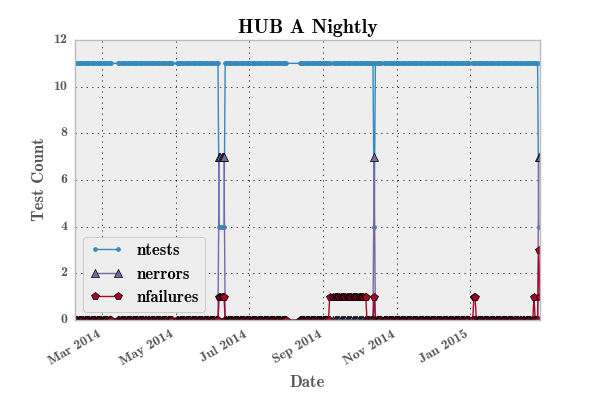
\includegraphics[width=\textwidth]{../../images/summary_plots/hub_a_nightly.png}
        \end{subfigure}
        \begin{subfigure}[b]{0.65\textwidth}
                \centering
                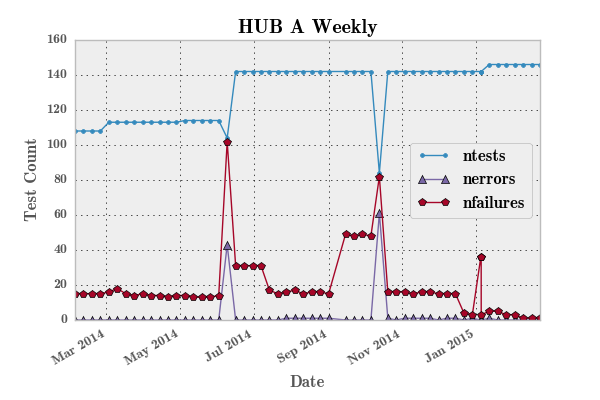
\includegraphics[width=\textwidth]{../../images/summary_plots/hub_a_weekly.png}
        \end{subfigure}
        \caption{ HUBcheck was used to track the health of hub A,
                  a \textit{Turbulent} hub, as website and tool session
                  container software were upgraded through 2014.
                  \textbf{ntests} represents the number of tests in the HUBcheck
                  test suite that ran and completed with either a pass
                  or fail status. \textbf{nerrors} represents the number of
                  HUBcheck tests that partially ran and exited due to
                  an exception being raised. In a small number of cases,
                  the exception is related to an error in the HUBcheck
                  library. An overwhelming amount of the time, these errors
                  signal a problem on the hub that prevented the test
                  from being properly setup. \textbf{nfailures} represents the
                  number of tests that completed and failed due to an
                  assertion.
                  }
        \label{fig:hub_a_health_plots}
\end{figure}


\textit{Turbulent} hubs are typically older hubs that have gone through a
number of software upgrades in the past, when the upgrade process was more
relaxed and testing was less of a priority.  Over the monitoring period, the
HUBcheck test suites were critical in helping the HUBzero team identify and
document problems on hubs as software was upgraded and machines were rebooted.
The history of one particularly turbulent hub, hub A, can be seen in
\Cref{fig:hub_a_health_plots}.

For hub A, tracking began on February 03, 2014 where, at that time, 15 of the
108 tests in the weekly test suite were failing. The testing and failures were
focused on the tool session container configuration. This was an area of active
concern for the team because hub A was in the middle of transitioning the
simulation tools running in containers using the Debian 6 operating system to
containers using the Debian 7 operating system.  Between March 2014 and June
2014, the weekly suite continued to identify 15 test failures.

% hubzero.org ticket \#5286
% hubzero.org ticket \#5317

A number of events occurred on hub A that contributed to its fluctuating
status.  The first manifested itself at the beginning of June 2014 and was
somewhat hidden by another event. The more obvious event at the beginning of
June 2014 shows up as a spike in test failures and errors in the weekly test
suite results. The spike was due to an emergency kernel security patch that
required the shutdown of a machine hosting tool session containers for hub A.
Hidden in the background of this spike was an increase of 17 additional test
failures that were associated with new parameter passing tests that had been
added to the weekly test suite that same week. The newly failing tests showed
that code to support parameter passing was not available on the hub. This is
likely due to the hub needing a website code update.  In the beginning of July
2014, a code update was performed and the next run of the weekly test suite
showed 15 of the 17 previously failing tests began to pass. The two remaining
failing parameter passing tests were identified as bugs in HUBzero's core
implementation and fixes for them are being deployed on various hubs.


% hubzero.org ticket \#6324 (noexec /home)

The second event that elevated test failures occurred at the beginning of
September 2014, when a miscommunication lead to a change in the system that was
not immediately obvious. Symptoms of the problem caused several HUBcheck tests
to fail in the weeks that followed. In the beginning of October 2014, the
problem was identified and fixed.

% hubzero.org ticket \#7079 (noexec /home)

Since October 2014, hub A has shown a decrease in test failures, signaling a
healthier hub. When major events do arise, they have been addressed quickly due
to rigorous monitoring of HUBcheck. For example, early in January 2015,
HUBcheck test failures uncovered a configuration change that occurred after a
system reboot. The HUBzero team was able to quickly identify and resolve the
problem before hub users were affected. With HUBcheck monitoring, hub A is on
its way to becoming like other \textit{Upgraded} hubs.

Turbulent hubs are not common for the HUBzero team. Recently, hubs
that would have been classified as turbulent have been taken down as
opposed to being put through the website code update process. For the
Turbulent hubs that remain in service, HUBcheck's test suites have
been used to monitor their health and work towards applying updates for website
code and tool container configurations.  To keep hubs from falling into this
state, the HUBzero team should continue to add tests to the test suites that
check hub component functionality.



\section{Upgraded Hubs}
\label{sec:solution_upgraded}
% explain the meaning of the category
% give an idea of how to identify a hub that fits into this category from the plots
% analyze the experience of one hub that is the representative for this category
% tell how hubs are moved out of this category to a better category.
% give recommendations on how to keep hubs from falling into this category.

% over the 20140201 - 20150201 monitoring period, pharmahub had 59 support tickets opened.
% 473 - launching tools blank page
% 472 - rappture gui problem with a tool, tool development question
% 459 - explain to user that rappture libraries moved, tool development question
% 458 - tool developement question, june 6 submit error found, problem was fixed in newer versions of submit, problem didn't seem to be related to original question.
% 457 - tool doesnt launch, had previously asked tool developer to update tool, but they didn't. tool development question
% 455 - need debian packages installed, tool development question.
% 453 - tool fails to launch, due to developers not upgrading after hub and container upgrade
% 420 - tools launch with unsigned applet, web issue
% 419 - install new R version, tool development question
% 

Most hubs have a hub health signature that resembles that of an
\textit{Upgraded} hub, where the HUBcheck weekly test suite results start off
with a number of test failures that steadily decrease over time. On
Upgraded hubs, increases in test failures may be seen at predictable
times, such as right after hub updates or during planned maintenance, making them
easy to identify and explain on the nightly and weekly suite result graphs.

\begin{figure}[ht!]
        \centering
        \begin{subfigure}[b]{0.65\textwidth}
                \centering
                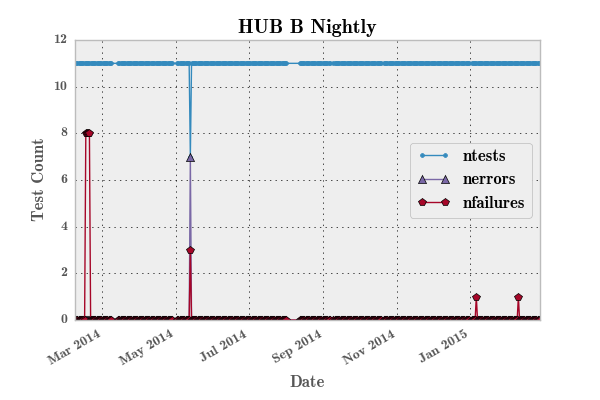
\includegraphics[width=\textwidth]{../../images/summary_plots/hub_b_nightly.png}
        \end{subfigure}
        \begin{subfigure}[b]{0.65\textwidth}
                \centering
                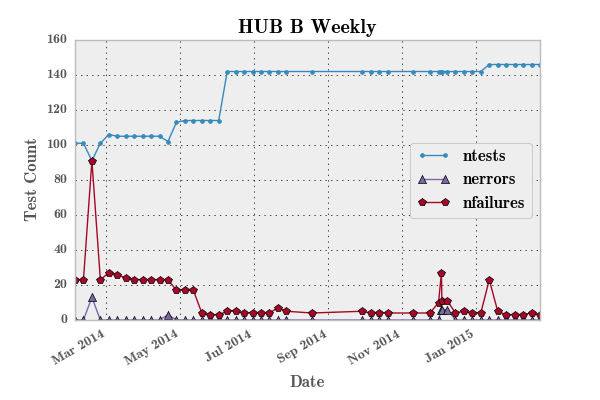
\includegraphics[width=\textwidth]{../../images/summary_plots/hub_b_weekly.png}
        \end{subfigure}
        \caption{ \textit{Upgraded} hubs, like hub B, have a much
                  smoother health graph, where, as time progresses
                  and the number of tests increase, the number of
                  failures decrease. }
        \label{fig:hub_b_health_plots}
\end{figure}

Hub B was brought online at about the same time as hub A. Prior to February
2014, it would have been identified as a \textit{Turbulent} hub due to its use
of vintage website code and tool session container configurations, but today it
is an example of an \textit{Upgraded} hub. The hub received a code update just
before the monitoring period began, but HUBcheck nightly and weekly suites were
still instrumental in helping to identify and fix many of the problems the hub
was experiencing before the upgrade. In February 2014, monitoring of hub B
reported 23 test failures until the end of April. Throughout April, the HUBzero
team focused on reducing test failures on hub B. By the end of April, the
number of failures had dropped from 23 to 17 as new tests were introduced into
the weekly test suite. This decreasing trend is again seen near the middle of
May, when the number of test failures dropped to 4 tests.  The weekly test
suite results graph shows that with the exception of a few false positives, the
number of failures holds steady at 4 tests through the end of November 2014.
In the beginning of December, the software on hub B was upgraded, and HUBcheck
alerted the HUBzero team to a configuration change that caused features on some
web pages to be rendered incorrectly.

The gradually decreasing trend of test failures seen between February and
December 2014 is characteristic of Upgraded hubs. Generally, bugs are
introduced to the system at predictable times such as during system upgrades or
machine reboots. By monitoring test failures through HUBcheck, the HUBzero team
is able to address old problems over time and quickly stamp out new problems.


% not sure what caused the first spike, might have been loosely related to
% hubzero \#4069 (ptys left open after SSH bash shells closed)

% hubzero \#6834 (missing tool session web page decorations after upgrade)

% Jan 12, 2015 - something bad happened to the x virtual frame buffer i think,
% causing false positives to show up for parameter passing tests


\section{New Hubs}
\label{sec:solution_new}
% explain the meaning of the category
% give an idea of how to identify a hub that fits into this category from the plots
% analyze the experience of one hub that is the representative for this category
% tell how hubs are moved out of this category to a better category.
% give recommendations on how to keep hubs from falling into this category.

% datacenterhub - 11/03 spike from switching locators on website without updating hubcheck
% mygeohub - 07/02 spike (hubzero #5511) combining hub data
%          - 11/17 spike fixed by updating hubcheck locators
% polytechhub
% 

\textit{New} hubs are the easiest of hubs to identify. Their nightly and weekly
test suite results start off with nearly zero test failures and over time, new
failures rarely occur. Hubs categorized as New hubs can be reclassified as
Upgraded hubs after they go through a code update cycle. Newly instantiated
hubs managed by the HUBzero team receive a code update on a set schedule of
about every month. This strategy keeps the hubs up to date with bug fixes and
contributes to the reduced number of failures seen in HUBcheck's results.


\begin{figure}[ht!]
        \centering
        \begin{subfigure}[b]{0.65\textwidth}
                \centering
                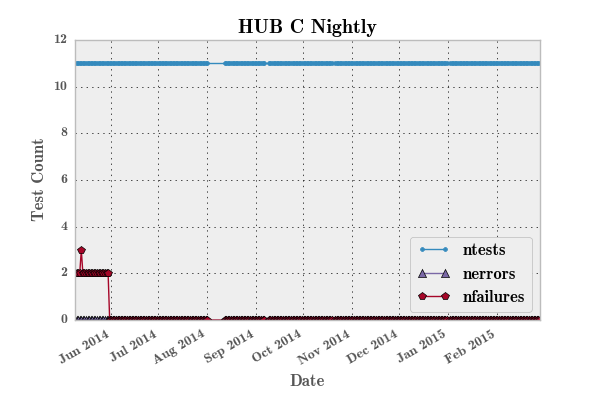
\includegraphics[width=\textwidth]{../../images/summary_plots/hub_c_nightly.png}
        \end{subfigure}
        \begin{subfigure}[b]{0.65\textwidth}
                \centering
                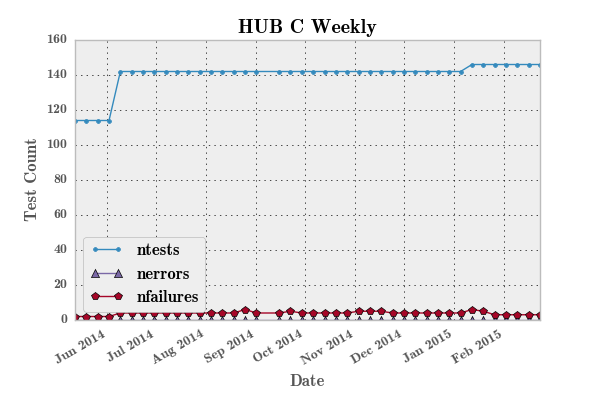
\includegraphics[width=\textwidth]{../../images/summary_plots/hub_c_weekly.png}
        \end{subfigure}
        \caption{For \textit{New} hubs, like hub C, once the setup has completed,
                 the main source of test failures is known problems
                 in the HUBzero's core software.}
        \label{fig:hub_c_health_plots}
\end{figure}


In 2014, the HUBzero team brought up five new hubs.  After the initial setup
was complete, each hub's weekly test suite results showed that the number of
test failures was kept at a steady rate, with nearly all failures being
categorized as known bugs, planned failures, or false positives.

Hub C is was one of the first hubs to be launched in 2014. Since May 2014, hub
C's weekly suite results graph has consistently reported under seven failures.
In June 2014, after additional tests were added to the weekly suite, the number
of test failures rose very slightly due to the identification of known bugs in
the HUBzero software.  Through out September 2014 and November 2014, four false
positives crept up, but for the most part, errors identified by HUBcheck have
stayed very low since the launch of the hub.

New hubs start off with the benefit of being installed with the latest hub code
and configurations. Over time, new features are introduced to the HUBzero
software, bugs are fixed, and the new hubs need to be updated. Consistent
updates and automated tests performed by HUBcheck help keep new hubs working
properly.


% Recommendations are optional.
% You may include recommendations as a major division if your
% subject matter and research dictate.
% Reference: TM 32.
% CHANGE NEXT LINE?
%
%  recommendations.tex  2007-02-06  Mark Senn  http://www.ecn.purdue.edu/~mark
%

% incorporate hubcheck into the development process. at the very least, when we
% roll out a new feature or component on the hub, we should be asking "what is
% the test plan". it also helps to have light documentation or requirements
% describing how the component is supposed to work. these requirements are the
% basis for hubcheck tests.
%
% selenium is not the only website checking software out there. other web
% automation libraries can be used instead. the work done in hubcheck can be
% used as a proof of concept and can possibly be applied to other software.
%
% with respect to building more page objects and testing more web components,
% the hubzero team should probably make it a priority to focus on building
% tests for one component at a time since resources seem to be streached and
% the team has already published components that don't have an automated
% testing plan.
%
% it would also help if the team had test environments where developers would
% quickly build a clean version of the hub, running the recommended setup or a
% clone of one of our existing hubs. the developer could then load their new
% software on this test system and run hubcheck against the test system. the
% hubcheck tests should include tests for their new feature so they can make
% sure their code works, as well as tests from previously accepted components
% to make sure the new feature works with the currently stable code.
%
% recommendations and future work for hubcheck.
%
% incorporate googletest or some other framework for testing Rappture's C/C++
% code.
%
% currently hubcheck makes it very easy to use pre-installed page objects and
% very hard to use page objects that are not a part of the standard
% installation. this limits the user's ability to build and use page objects
% for web pages other than the hub when using hubcheck. hubcheck libraries can
% be used for websites that are not hubs. it should be easier for users to
% build page objects that they store locally, outside of the standard
% installation, and use with their own scripts.
%
% like to separate the hubcheck tests and hub page objects from the hubcheck
% library.
%
% finish the hubcheck.bashshell module which builds upon the pexpect module, a
% python implementation of Tcl's Expect. the hubcheck.bashshell module aims to
% implement an interface similar to that of the hubcheck.sshshell module,
% providing the usual send() and expect() methods, but also provides an
% execute() method. the execute() method can run small scripts in the form of a
% list of commands, checking the exit status of each command, and optionally
% raising an exception if a command fails. this method reduces the usual cycle
% of sending a command, expecting a result, sending another command to check
% the exit status, and expecting the exit status, down to a single method call
% with the command or list of commands that should be run.


% future work
% 1. hubcheck library improvements.
%   0. **creating test accounts and storing passwords**
%   a. additional modules (bashshell)
%   b. organization (split library, pageobjects, tests)
%   c. standard installation using system packages
% 2. improving the testing environment.
%   a. incorporate hubcheck earlier in the development cycle.
%   b. encourage repeated automated testing. once it is setup, its easy to keep doing.
% 3. evangelizing hubcheck to the hubzero team.
%   a. show people how to use hubcheck during their own development.
%   b. encourage people to write their own page objects and tests, and contribute them to the library.
%   c. get people thinking about planning for automated testing while they develop.


\chapter{FUTURE WORK}
\label{chap:future}

The future of HUBcheck is full of opportunities ranging from core library
improvements, to the manifestation of robust test environments, to evangelizing
HUBcheck to the HUBzero Team.

\section{Library Improvements}
\label{sec:future_library}

The HUBcheck library's shell modules are based on the assumption that tests
will be performed in a tool session container over SSH, but having access to a
bash shell on the local machine could open up alternative ways of running
testing currently unavailable to HUBcheck. With local shell access, HUBcheck
could be installed on a hub and run as a user to perform tests without needing
to navigate layers of authentication, reducing false positives stemming from
expired passwords and revoked SSH access. The current bash shell module
template, \xfmodule{hubcheck.bashshell}, builds upon the \xfmodule{pexpect}
module, a Python implementation of Tcl's Expect. The
\xfmodule{hubcheck.bashshell} module aims to implement an interface similar to
that of the \xfmodule{hubcheck.sshshell} module, providing the usual
\xfmethod{send()} and \xfmethod{expect()} methods, but also provides an
\xfmethod{execute()} method described in
\Cref{ssec:hubcheck_shell_modules_interacting_containers}.


The organization of the HUBcheck library could also be improved. Currently, the
core HUBcheck library, HUBzero specific page objects, and tests are all kept in
the same repository and installed together. A better setup would be to install
the core library and allow the HUBzero specific page objects to exist in a
different location. This separation would also make it easier for users to
build and use their own page objects while using the core HUBcheck library as
a frame for developing automation scripts. The tests should be installed in a
separate location, making them easy to update and add to without the need to
reinstall the whole HUBcheck library.

A reorganization of the HUBcheck library should be performed in coordination
with a standardization of the HUBcheck install process. HUBcheck installations
should try to use system libraries whenever possible instead of shipping with
its own copies of libraries to reduce the propagation of security bugs.

\section{Test Environments}
\label{sec:future_testenv}

HUBcheck is one piece of the larger testing puzzle that the HUBzero Team is
trying to solve. The placement of HUBcheck in the development cycle is a bit
off. Right now, it runs on live hubs managed by the HUBzero Team because other
available systems that are used for testing fall short in possessing the
properties of a true testing environment that (1) represents a production
environment, (2) is easily reproducible, and (3) is reliably available.
Developers need a test environment they can quickly launch with a production
compatible hub installation, update with a new feature being developed, and run
HUBcheck tests. This falls in line with the goals of the HUBcheck project of
lowering the barriers to adopting better testing practices earlier in the
development cycle.

\section{Adoption Within the HUBzero Team}
\label{sec:future_adoption}

Another missing piece to the HUBcheck project is an educational component.
Using and setting up HUBcheck to run is undocumented for the most part. Future
work will include evangelizing for HUBcheck, and better testing practices in
general. HUBcheck is not the correct tool for all problems, but fits a unique
niche within the hub environment that discouraged testing in the past and left
hubs in a precarious state. The HUBcheck project helps promote one of the core
phases in the software development process.


% Appendices are optional.
% Appendices are not necessarily part of every thesis. Appendices are used
% for supplementary illustrative material, original data, computer programs,
% and other material not necessarily appropriate for inclusion within the
% text of your thesis. 
% Reference: TM 33.
% Use "\appendix" for one appendix or "\appendices" for more than one
% appendix.
% CHANGE NEXT 7 LINES?
%\appendices
%\include{basepageelements}
%\include{parameter_pass_testing}
%%\include{demo-citations}
%%\include{demo-figures}
%%\include{demo-mathematics}
%%\include{demo-multicols}
%%\include{demo-tables}
%%\include{demo-text}

% Bibliography is required if you consulted any outside references.
% Reference: TM 32.
%
%  bibliography.tex     June 3, 2002     Mark Senn
%
%  This is the bibliography for a simple, example thesis.
%

\bibliography{all}
%\bibliographystyle{plain}


% Notes and footnotes are optional.
% Reference: TM 34.
% I have not implemented this yet.  Mark Senn 2002-06-03
%%\include{notes}

% A vita is optional for masters theses
% and required for doctoral dissertations.
% Reference: TM 13.
% CHANGE NEXT LINE?
%%\include{vita}

\end{document}

% LaTeX won't read after the \end{document} command.
% You can put notes to yourself or LaTeX input not
% ready for use here if you'd like.
